%%
%% fourier.tex
%% 
%% Made by Alex Nelson
%% Login   <alex@tomato>
%% 
%% Started on  Wed Dec 17 14:47:32 2008 Alex Nelson
%% Last update Sat Jan  3 16:59:46 2009 Alex Nelson
%%
\documentclass[10pt,draft,twoside]{article}
\usepackage{makeidx} % for the index e.g. \index{key}
\makeindex
\usepackage{fly,brackets}
\usepackage{subfigure,plain}
\usepackage{wrapfig} % used for wrapping figures!

\newcommand\mbf[1]{\mathbf{#1}} % simplify writing in math bold font
\numberwithin{figure}{section}
\title{Notes on Fourier Analysis}
\date{December 17, 2008}
\author{pqnelson@gmail.com}
\begin{document}
\maketitle
\tableofcontents
\listoffigures
%%
%% fourierIndex.tex
%% 
%% Made by Alex Nelson
%% Login   <alex@tomato>
%% 
%% Started on  Fri Dec 19 22:15:05 2008 Alex Nelson
%% Last update Sat Jan  3 15:42:05 2009 Alex Nelson
%%
%% TODO: I need to do some more work on Fourier transforms 
%%
\part{Fourier Series}
\section{Differential Equations: A Motivation for Fourier Series}
%%
%% 31March2008.tex
%% 
%% Made by Alex Nelson
%% Login   <alex@tomato>
%% 
%% Started on  Wed Dec 17 12:33:29 2008 Alex Nelson
%% Last update Sat Jan  3 16:35:11 2009 Alex Nelson
%%

\begin{ex}{(Diffusion of heat in solid body)}

The initial motivation behind Fourier series was to solve the
heat equation. The specific problem was trying to model the flow
of heat in a thin metal rod, such as the one seen in figure
\eqref{fig:31March2008img1}. The equation describing it requires
us first to consider several variables. For simplicity, consider
only a one dimensional ``thing'' insulated metal rod with length
$L$. 

\begin{figure}[h!]
  \begin{center}
    %%
%% 31March2008img1.tex
%% 
%% Made by Alex Nelson
%% Login   <alex@tomato>
%% 
%% Started on  Wed Dec 17 12:41:25 2008 Alex Nelson
%% Last update Wed Dec 17 12:41:25 2008 Alex Nelson
%% 2.1875in
\setlength{\unitlength}{0.0125in}
\begin{picture}(175,50)(0,-20)
\thinlines
\put(20,20){\circle{9}} % one end of the rod
\put(150,20){\arc{10}{5}{1}} % the other end of the rod
\drawline(0,0)(165,0) % the x axis
\drawline(21,24)(152,25) % the top of the rod
\drawline(21,16)(152,15) % the bottom of the rod
\dottedline{3}(20,16)(20,0) % the dashed bit to $x=0$
\dottedline{3}(152,16)(152,0) % dashed bit to $x=L$
\put(17,-10){\makebox(0,0)[lb]{\raisebox{0pt}[0pt][0pt]{\twltt $0$}}}
\put(147,-10){\makebox(0,0)[lb]{\raisebox{0pt}[0pt][0pt]{\twltt $L$}}}
\put(170,-3){\makebox(0,0)[lb]{\raisebox{0pt}[0pt][0pt]{\twltt $x$}}}
\end{picture}

  \end{center}
\caption{A thin insulated metal rod of length $L$}
\label{fig:31March2008img1}
\end{figure}

We can describe the problem with some conditions\index{Heat Equation}
\begin{subequations}
\begin{align}
u(x,t) &= \text{temperature at point $x$ and time $t$} \\
u(x,0) &= f(x)\quad (\text{temperature at time $t=0$, initial
  condition}) \\
u(0,t) = u(L,t) &= 0 \quad(\text{boundary condition})
\end{align}
\end{subequations}
Observe that we hold the temperature at the endpoints fixed to be
zero at all time. This is weird physically, because we rarely see
such a system. So we can describe the heat flow in a thin metal
rod by the equation
\begin{equation}\label{eq:31March2008:HeatEqn}
\frac{\partial u}{\partial t} = k\frac{\partial^{2}u}{\partial
  x^{2}}
\end{equation}
where $k$ is the diffusitivity of the rod (how quickly heat can
spread), and this is known as the heat equation. Now that we have
described the dynamics of the heat flow for this thin metal rod,
solving it should be trivial...right? 

Well, without
the boundary conditions and initial conditions, one can struggle
\marginpar{Skip work, here's answer}for a long long long time to find that
\begin{equation}\label{eq:31March2008:solution}
u(x,t) = t^{-1/2}\exp\left(\frac{-x^{2}}{4kt}\right)
\end{equation}
is a solution for $t>0$. So we would just need to solve the
boundary value problem. This is not as trivial as it seems.
\end{ex}

Our toolkit from taking basic differential equations (which is:
``Guess really really good!'') is inadequate to solve this
problem. We need to introduce a new
technique\marginpar{seperation of variables} which we call
\textbf{seperation of variables}. What we do is we assume we can
write the function $u(x,t)$ as
\begin{equation}\label{eq:31March2008:seperationOfVariables}
u(x,t)=X(x)T(t)
\end{equation}
This usually works but not always\footnote{It should be noted
  that this is a coordinate-choice, so there are a finite number
  of coordinate systems we can do this in (e.g. Morse et
  al.~\cite{morseVolTwo} point out that the Hemholtz equation,
  for example, can only be solved via seperation of variables in
  11 coordinate systems).}. We will not investigate it here but
it should be noted that it may not always work.

The second step to the ``seperation of
variables''\index{Seperation of Variables} technique is
to plug in \eqref{eq:31March2008:seperationOfVariables} into the
differential equation
\begin{subequations}
\begin{align}
\partial_{t} u(x,t) &= k\partial_{x}^{2}u(x,t) \\
\partial_{t} (X(x)T(t)) &= k\partial_{x}^{2}(X(x)T(t)) \\
X(x)T'(t) &= kX''(x)T(t)
\end{align}
\end{subequations}
and at first this seems useless. What do we do with this result?
Well, we divide both sides by $kX(x)T(t)$ and set it to be equal
to some constant\marginpar{Don't believe it? Note the left
  equation is independent of $x$, the middle equation is
  independent of $t$, so take the $t$ derivative of
  everything and you get the middle equation being 0,
  similar results for the $x$ derivative imply that they're
  equal to some constant.}
\begin{equation}
\frac{T'(t)}{kT(t)} = \frac{X''(x)}{X(x)}
= \begin{pmatrix}$some$\ $constant$\\$to$\ $be$\ $determined$\end{pmatrix}
\end{equation}
Observe that we have on the left hand side a function of $t$
only, it is independent of $x$. Similarly, the middle term is
independent of $t$. That is, we note
\begin{equation*}
\underbracket[0.5pt]{\frac{T'(t)}{kT(t)}}_{\text{independent of $x$}} =
\underbracket[0.5pt]{ \frac{X''(x)}{X(x)}}_{\text{independent of $t$}} =  \begin{pmatrix}$some$\ $constant$\\$to$\ $be$\ $determined$\end{pmatrix}
\end{equation*}
Now, we can solve for the general solution of $T(t)$
\begin{equation}
\frac{T'(t)}{T(t)}=kA\Rightarrow \log|T(t)|=kAt +
c_{1}\Rightarrow T(t)=T_{0}e^{kAt}
\end{equation}
where $T_{0}=T(0)$ is some constant.                            

Now, for solving $X(x)$, we have a bit more difficult of a
problem. The differential equation of relevance is
\begin{equation}
\frac{X''(x)}{X(x)} = A\Rightarrow X''(x) - AX(x) = 0
\end{equation}
Recall for general second order differential equations
\begin{equation}
y'' + ay' + by = 0
\end{equation}
we have the \textbf{characteristic equation}\index{Characteristic Equation!Differential Equations}
\begin{equation}
r^{2} + ar + b = 0.
\end{equation}
It has two roots, by the fundamental theorem of
Algebra\marginpar{Fundamental Thm Of Algebra: A polynomial
  of degree $n$ has exactly $n$ complex roots}. So we have
the two roots $r_{1}$ and $r_{2}$ which gives us that
general solution
\begin{equation}
y(x) = c_{1}e^{r_{1}x} + c_{2}e^{r_{2}x}.
\end{equation}
For us, we have a simple characteristic equation
\begin{equation}
r^{2} - A = 0\Rightarrow r = \pm\sqrt{A}
\end{equation}
thus the general solution is
\begin{equation}
X(x) = c_{1}e^{x\sqrt{A}} + c_{2}e^{-x\sqrt{A}}
\end{equation}
\marginpar{What's $A$?}So now we have a new problem: what
values of $A$ give nonzero solutions? That is, which ones
satisfy the boundary conditions
\begin{equation}
X(0)=X(L)=0
\end{equation}
without $X(x)$ being trivial (i.e. $X(x)=0$).

If $A>0$, then we have by one boundary condition
\begin{equation}
X(0)=c_1 + c_2=0\Rightarrow c_1 = -c_2.
\end{equation}
And by the other boundary condition
\begin{equation}
X(L) = c_{1}e^{L\sqrt{A}}+c_{2}e^{-L\sqrt{A}} = 0\Rightarrow
c_{1}e^{2L\sqrt{A}}+c_{2}=0
\end{equation}
and by putting these two together we find
\begin{equation}
c_{1}(1 - e^{2L\sqrt{A}}) = 0
\end{equation}
which requires either $c_1=0$ or $\exp(2L\sqrt{A})=1$. The
latter implies either $L=0$ or $A=0$. We assumed that $L>0$
and $A>0$. So that implies $c_1=0$. Thus the general
solution is
\begin{equation}
X(x) = c_{2}e^{-x\sqrt{A}}
\end{equation}
which is really just exponential decay.

For the $A<0$ case, the general solution can be written as
\begin{equation}
X(x) = c_{1}\cos(\lambda x) + c_{2}\sin(\lambda x)
\end{equation}
where $\lambda=\sqrt{-A}$. We plug in the boundary
conditions
\begin{equation}
X(0) = c_1 = 0
\end{equation}
and
\begin{equation}
X(L) = c_{2}\sin(\lambda L) = 0\Rightarrow \lambda L = n\pi
\Rightarrow \lambda = \frac{n\pi}{L}
\end{equation}
where $n\in\mathbb{Z}$. So here we have $A=-n^{2}\pi^{2}/L^{2}$.

Putting this all together, the general solution to the
boundary value problem is
\begin{equation}
u_{n}(x,t) =
\left(c_{0}\exp(-k\frac{n^{2}\pi^{2}}{L^{2}}t)\right)\left(c_{1}\sin(\frac{n\pi}{L}x\right)
\end{equation}
But also observe that \emph{any linear combinations} of
these solutions \emph{are also solutions} to the boundary
value problem. So the general solution is
\begin{equation}\label{eq:31March2008:generalSolutionUsingSeries}
u(x,t) =
\sum^{\infty}_{n=1}a_{n}e^{-kn^{2}\pi^{2}t/L^{2}}\sin\left(\frac{n\pi}{L}x\right)
\end{equation}
where $a_{n}$ are arbitrary constants.

``\emph{How to make $u(x,t)$ satisfy the initial condition
  $u(x,0)=f(x)$?}'' Well, we have a small substitution to
make, we just set
\eqref{eq:31March2008:generalSolutionUsingSeries} equal to
the given boundary condition
\begin{equation}
\sum^{\infty}_{n=1}a_{n}\sin\left(\frac{n\pi}{L}x\right) =
f(x)
\end{equation}
\emph{This is where Fourier works his magic, expanding a
  function in terms of sines and cosines.} \marginpar{Point
  to ponder}Is it possible to find an expansion for \emph{any} heat distribution?

\section{A First Look at Fourier Series}
%%
%% 2April2008.tex
%% 
%% Made by Alex Nelson
%% Login   <alex@tomato>
%% 
%% Started on  Wed Dec 17 15:47:14 2008 Alex Nelson
%% Last update Wed Dec 17 15:47:14 2008 Alex Nelson
%%

Remember Euler's formula
\begin{equation}
e^{i\theta} = \cos(\theta)+i\sin(\theta).
\end{equation}
Observe that
\begin{equation}
e^{-i\theta}=e^{i(-\theta)} = \cos(-\theta)+i\sin(-\theta)
\end{equation}
and
\begin{equation}
\overline{e^{i\theta}}=e^{-i\theta} =
\cos(\theta)-i\sin(\theta).
\end{equation}
We set $e^{-i\theta}=e^{-i\theta}$ and find from the real
part
\begin{equation}
\cos(-\theta)=\cos(\theta)
\end{equation}
and from the imaginary part
\begin{equation}
\sin(-\theta)=-\sin(\theta).
\end{equation}
We call $\cos(\theta)\approx 1-\theta^2/2+...$ an \textbf{even function} and
$\sin(\theta)\approx \theta-\theta^3/6+...$ an \textbf{odd function}. 

\begin{defn}
Let $f:\mathbb{R}\to\mathbb{R}$ be a function, then $f$ is
\textbf{periodic with period $p$} (or $p$-\textbf{periodic})
if
\begin{equation}
f(x+p)=f(x)
\end{equation}
holds.
\end{defn}

\begin{ex}
The functions $\cos(\theta)$, $\sin(\theta)$ and
$\exp(i\theta)$ are all $2\pi$-periodic.
\end{ex}

\begin{lem}
If we have a $p$-periodic function $f$, then
\begin{equation}
\int^{a+p}_{a}f(x)dx
\end{equation}
is independent of $a$.
\end{lem}
\begin{proof}
If we change $a$ by some $c$ (so $a\to a+c$) then
\begin{subequations}
\begin{align}
\int^{a+c+p}_{a+c}f(x)dx &= \int^{a+p}_{a+c}f(x)dx +
\int^{a+c+p}_{a+p}f(x)dx\quad(\text{by linearity of integral})\\
&= \int^{a+p}_{a+c}f(x)dx +
\int^{a+c}_{a}f(x)dx\quad(\text{by periodicity of $f(x)$}) \\
&= \int^{a+p}_{a}f(x)dx\quad(\text{collecting terms})
\end{align}
\end{subequations}
where we justify the second step (the one justified in a
handwavy way with the ``periodicity of $f$'') by using the
Riemann sum and noting such reasoning works for that
particular definition of the integral and we use it here too.
\end{proof}

\begin{defn}
Let $f:\mathbb{R}\to\mathbb{R}$ be $2\pi$-periodic and
integrable on $[-\pi,\pi]$. The \textbf{Fourier Series} $f$
is
\begin{equation}
f(\theta)=\sum^{\infty}_{n=-\infty}c_{n}e^{in\theta}
\end{equation}
where
\begin{equation}
c_{n} =
\frac{1}{2\pi}\int^{\pi}_{-\pi}f(\theta)e^{-i\theta}d\theta
\end{equation}
is called the \textbf{Fourier Coefficient}\index{Fourier Coefficient} of $f$.
\end{defn}

\begin{rmk}
This is called the ``\textbf{exponential form}'' of the\index{Fourier Coefficient!Exponential Form}
Fourier Series. There are other forms of the Fourier series.
\end{rmk}

We can equivalently write the Fourier series in a slightly
different approach,
\begin{equation}
f(\theta) = \frac{1}{2}a_{0} +
\sum^{\infty}_{n=1}(a_{n}\cos(n\theta)+b_{n}\sin(n\theta))
\end{equation}
where
\begin{subequations}
\begin{align}
a_{0} &= \frac{1}{\pi}\int^{\pi}_{-\pi}f(\theta)d\theta \\
a_{n} &=
\frac{1}{\pi}\int^{\pi}_{-\pi}f(\theta)\cos(n\theta)d\theta\\
b_{n} &=
\frac{1}{\pi}\int^{\pi}_{-\pi}f(\theta)\sin(n\theta)d\theta
\end{align}
\end{subequations}
Observe that
\begin{subequations}
\begin{align}
a_{n}
&=\frac{1}{\pi}\int^{\pi}_{-\pi}f(\theta)\left(\frac{e^{in\theta}+e^{-in\theta}}{2}\right)d\theta
\\
&=
\frac{1}{2\pi}\int^{\pi}_{-\pi}f(\theta)(e^{in\theta}+e^{-in\theta})d\theta
\\
&= c_{n}+c_{-n}
\end{align}
\end{subequations}
and
\begin{subequations}
\begin{align}
b_{n} &=
\frac{1}{\pi}\int^{\pi}_{-\pi}f(\theta)\left(\frac{e^{in\theta}-e^{-in\theta}}{2i}\right)d\theta
\\
&=
\frac{1}{2\pi}\int^{\pi}_{-\pi}f(\theta)(e^{in\theta}-e^{-in\theta})d\theta
\\
&= i(c_{n}-c_{-n})
\end{align}
\end{subequations}
thus putting it all together we get
\begin{equation}
c_{n} = \frac{a_{n}-ib_{n}}{2}.
\end{equation}
So really, we are starting to see a connection between the
two forms.

The equivalence of the two forms can be explicity written
\begin{subequations}
\begin{align}
\sum^{\infty}_{n=-\infty}c_{n}e^{in\theta} &= c_{0} +
\sum^{\infty}_{n=1}c_{n}e^{in\theta} + c_{-n}e^{-in\theta}
\\
&= c_0 +
\sum^{\infty}_{n=1}c_{n}(\cos(n\theta)+i\sin(n\theta))+c_{-n}(\cos(n\theta)-i\sin(n\theta)
\\
&= c_{0} + \sum^{\infty}_{n=1} (c_{n}+c_{-n})\cos(n\theta) +
i(c_{n}-c_{-n})\sin(n\theta) \\
&= c_{0} + \sum^{\infty}_{n=1}a_{n}\cos(n\theta) +
b_{n}\sin(n\theta) \\
&= \frac{a_{0}}{2} + \sum^{\infty}_{n=1}a_{n}\cos(n\theta) + b_{n}\sin(n\theta)
\end{align}
\end{subequations}
which explicitly demonstrates the equivalence between the
two forms.

\subsection{Derivation of Definition of Fourier Series}

We want to expand our periodic function in terms of sines
and cosines
\begin{equation}
f(\theta) = \sum^{\infty}_{n=-\infty}c_{n}e^{in\theta}
\end{equation}
So...what is $c_{n}$?\index{Fourier Coefficient} Well, first we should probably
remember that
\begin{equation}
\int^{\pi}_{-\pi}e^{inx}e^{-inx}dx = \int^{\pi}_{-\pi}dx =
2\pi
\end{equation}
and if $m\in\mathbb{Z}$ such that $m\neq 0$ then
\begin{subequations}
\begin{align}
\int^{\pi}_{-\pi}e^{inx}e^{-i(n+m)x}dx &=
\int^{\pi}_{-\pi}e^{-imx}dx\\
&= \frac{1}{-im}(e^{-im\pi}-e^{im\pi}) \\
&= \frac{i}{m}( (e^{-i\pi})^{m}-(e^{i\pi})^{m}) \\
&= \frac{i}{m}( (-1)^{m} - (-1)^{m}) \\
&= \frac{i}{m}(0) = 0.
\end{align}
\end{subequations}
So we found in general
\begin{equation}
\int^{\pi}_{-\pi}e^{inx}e^{-imx}dx = 2\pi\delta_{mn}
\end{equation}
where $\delta_{mn}$ is the kronecker delta (it is 1 if $m=n$
and 0 otherwise).

So, if we then take
\begin{equation}
f(x) = \sum^{\infty}_{n=-\infty}c_{n}e^{inx}
\end{equation}
then
\begin{subequations}
\begin{align}
\int^{\pi}_{-\pi}f(x)e^{-ikx}dx &=
\sum^{\infty}_{n=-\infty}c_{n}\int^{\pi}_{-\pi}e^{inx}e^{-ikx}dx\\
&=\sum^{\infty}_{n=-\infty}(2\pi\delta_{kn})c_{n} \\
&=(2\pi\cdot1)c_{k} + \sum_{n\neq k}(2\pi\cdot 0)c_{n} \\
&=(2\pi)c_{k}
\end{align}
\end{subequations}
so we conclude that
\begin{equation}
c_{k} = \frac{1}{2\pi}\int^{\pi}_{-\pi}f(x)e^{-ikx}dx
\end{equation}
which we already knew.

\begin{rmk}
We can also define Fourier coefficients in a slightly
different way. Instead of
\begin{equation}
c_{n} = \frac{1}{2\pi}\int^{\pi}_{-\pi}f(x)e^{-inx}dx
\end{equation}
we can equivalently write
\begin{equation}
c_{n} = \int^{1}_{0}f(x)e^{i2\pi nx}dx
\end{equation}
where $f$ becomes periodic with period 1.
\end{rmk}
\begin{rmk}
The Fourier coefficients are constant, and the constant
Fourier coefficient 
$$ c_0 = \frac{1}{2}a_{0} =
\frac{1}{2\pi}\int^{\pi}_{-\pi}f(x)dx $$
gives us the average value of $f$ over a $2\pi$ interval.
\end{rmk}

%% \begin{ex}
%% Let $f$ be a 2$\pi$ periodic function given by
%% \begin{equation}
%% f(\theta)=|\theta|,\qquad -\pi\leq\theta\leq\pi
%% \end{equation}
%% \begin{sagesilent}
%% l = line([(-3*pi,0),(-2*pi,1)])+line([(-2*pi,0),(-pi,1)])+line([(-pi,0),(0,1)])+line([(0,0),(pi,1)])+line([(pi,0),(2*pi,1)])+line([(2*pi,0),(3*pi,1)])
%% \end{sagesilent}
%% \sageplot{l.plot()}

%% \end{ex}
\begin{ex}
Let $f$ be a 2$\pi$ periodic function given by
\begin{equation}
f(\theta)=|\theta|,\qquad -\pi\leq\theta\leq\pi
\end{equation}
which is shown in figure \ref{fig:2April2008:triangleWave}.
\begin{figure}
\begin{center}
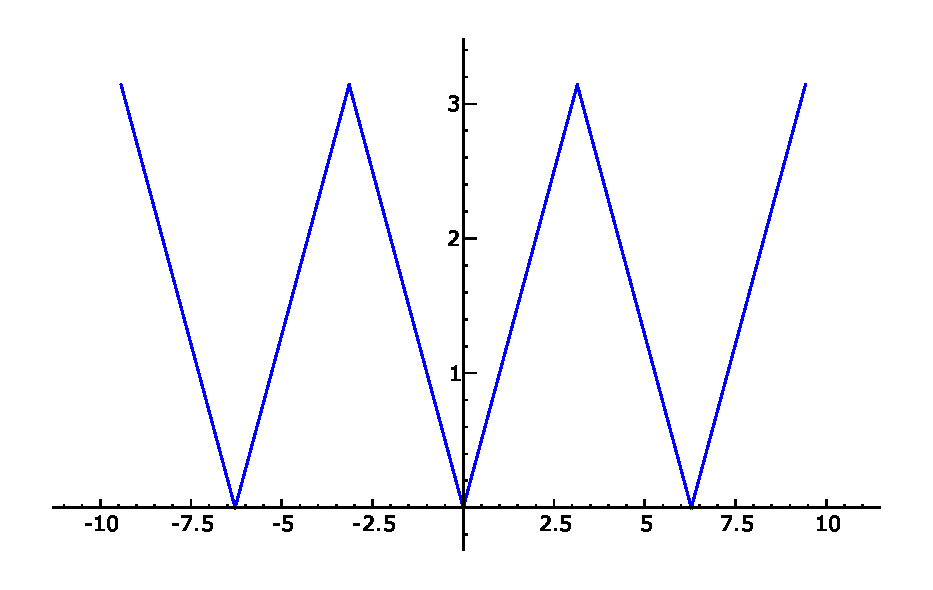
\includegraphics[width=\textwidth]{$HOME/book/fourier/img/2April2008triangleWave.eps}
\end{center}
\caption{The Triangle Wave.}
\label{fig:2April2008:triangleWave}
\end{figure}
We can calculate its Fourier series simply by using the
$a_n$ and $b_n$ cofficients. Observe
\begin{subequations}
\begin{align}
a_{0} &= \frac{1}{\pi}\int^{\pi}_{-\pi}f(\theta)d\theta \\
&= \frac{1}{\pi}\left(\int^{\pi}_{0}\theta d\theta +
\int^{0}_{-\pi}-\theta d\theta\right) \\
&= \frac{2}{\pi}\int^{\pi}_{0}\theta d\theta \\
&= \frac{2}{\pi}\left(\frac{\theta^2}{2}\Big|^{\pi}_{0}\right)\\
&= \frac{2}{\pi}\left(\frac{\pi^2}{2}\right) \\
&= \pi
\end{align}
\end{subequations}
Also observe that
\begin{equation}
f(-\theta)=f(\theta)
\end{equation}
so the $b_{n}=0$ for all $n\in\mathbb{Z}$. The only
coefficients we have to calculate are the $a_{n}$. Observe
\begin{subequations}
\begin{align}
a_{n} &=
\frac{2}{\pi}\int^{\pi}_{0}\theta\cos(\theta)d\theta \\
&=\frac{\pi}{2}\left[\frac{\theta\sin(n\theta)}{n}\Big|^{\pi}_{0}-\int^{\pi}_{0}\frac{\sin(n\theta)}{n}d\theta\right]\\
&=\frac{2}{\pi}\left[\left(0\right)+\frac{\cos(n\theta)}{n^2}\Big|^{\pi}_{0}\right] \\
&= \frac{2}{\pi}\left(\frac{(-1)^{n}-1}{n^{2}}\right) \\
&= \begin{cases} 0\qquad \text{$n$ is even} \\
-4/(n^2\pi)\qquad\text{$n$ is odd} 
\end{cases}
\end{align}
\end{subequations}
Now we can plug these coefficients into the Fourier series
to find
\begin{subequations}\label{eq:2April2008:fourierSeriesAbsoluteTheta}
\begin{align}
f(\theta) &= \frac{a_0}{2} +
\sum^{\infty}_{n=1}a_{n}\cos(n\theta) \\
&= \frac{\pi}{2} - \frac{4}{\pi}\sum^{\infty}_{n=1}\frac{\cos((2n-1)\theta)}{(2n-1)^2}
\end{align}
\end{subequations}
Now that we have expanded it, the question becomes:
\emph{does the Fourier series converge?} The answer is
yes. We observe that $\cos(\theta)\leq 1$ and 
\begin{equation}
\frac{1}{(2n-1)^2}\leq\frac{1}{n^2}
\end{equation}
thus term for term we have the inequality
\begin{equation}
\sum^{\infty}_{n=1}\frac{\cos((2n-1)\theta)}{(2n-1)^2} \leq \sum^{\infty}_{n=1}\frac{1}{n^2}.
\end{equation}
We know that $\sum 1/n^2$ converges (for a handwavy argument
if one is unconvinced: $\sum 1/n^2 \leq \int^{\infty}_{1}
(1/n^2)dn <\infty$ so the sum is finite), and our Fourier
series is less than this convergent sum, so it must converge
(by the Weierstrass M-test). 

% lambda x: (pi/2) - (4/pi)*sum([cos((2*k-1)*x)/((2*k-1)^2) for k in range(1,10)])

\begin{figure}[h]
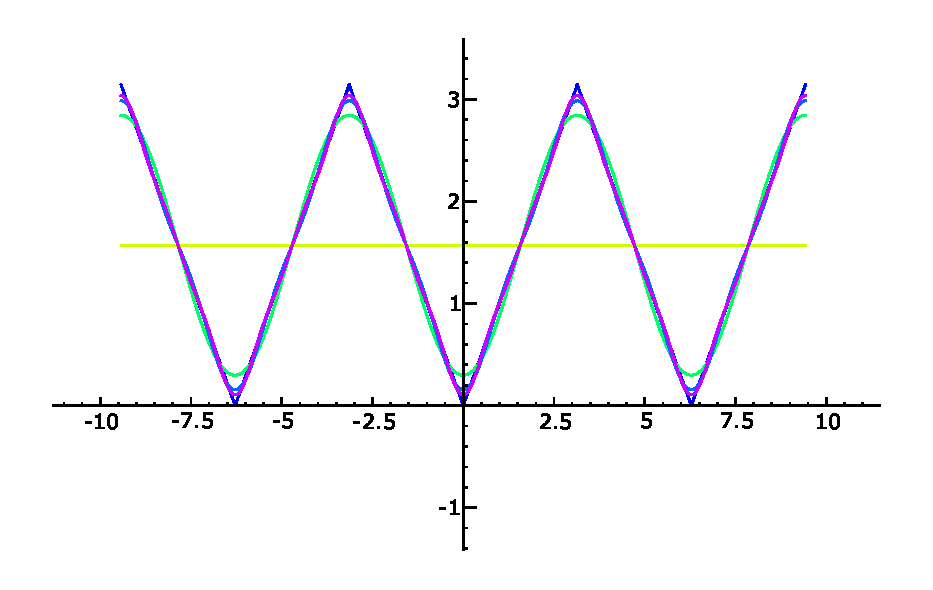
\includegraphics[width=\textwidth]{$HOME/book/fourier/img/2April2008img2.eps}
\caption[Partial Sums of Fourier Expansion of Triangle Wave]{The Partial sum to the Triangle wave with 1 through 5 terms. The actual triangle wave is shown in blue.}
\label{fig:2April2008:triangleWavePartialSum}
\end{figure}



\end{ex}

\section{Bessel's Inequality}
%%
%% 4April2008.tex
%% 
%% Made by Alex Nelson
%% Login   <alex@tomato>
%% 
%% Started on  Fri Dec 19 19:00:28 2008 Alex Nelson
%% Last update Fri Dec 19 19:00:28 2008 Alex Nelson
%%
%
%
% Bessel Inequality
%

\begin{bessel}\index{Bessel Inequality}
If $f$ is $2\pi$-periodic and Riemann integrable from $-\pi$
to $\pi$, and $c_n$ are the Fourier coefficients of $f$,
then 
\begin{equation}
\sum^{\infty}_{n=-\infty}|c_{n}|^2\leq\frac{1}{2\pi}\int^{\pi}_{-\pi}|f(\psi)|^2d\psi
< +\infty
\end{equation}
\end{bessel}

This is important because it allows us to create a bound for
the Fourier series that guarantees convergence. It should be
noted that equivalently it can be shown
\begin{equation}
\frac{1}{4}|a_0|^2 + \frac{1}{2}\sum^{\infty}_{n=1}|a_{n}|^2
+ |b_{n}|^{2} = \sum^{\infty}_{n=-\infty}|c_{n}|^{2} \leq \frac{1}{2\pi}\int^{\pi}_{-\pi}|f(\psi)|^2d\psi< +\infty.
\end{equation}
Why? Well, recall
\begin{subequations}
\begin{align}
a_{0} &= 2c_{0} \\
a_{n} &= c_{n} + c_{-n} \\ 
b_{n} &= i(c_{n}-c_{-n})
\end{align}
\end{subequations}
and also recall in complex analysis, $|z|^2 = z\bar{z}$ for
$z\in\mathbb{C}$. We would like
\begin{equation}
|a_{n}|^{2}\to 0\qquad\text{as } |n|\to\infty
\end{equation}
or
\begin{equation}\label{eq:4April2008:F1}
c_{n}\to 0\quad\text{as }|n|\to\infty.
\end{equation}
\marginpar{Riemann integrable and periodic?}The question
that arises is ``What kind of functions are Riemann
integrable and $2\pi$-periodic?''

Let us first review a number of definitions which will
simplify our life quite a bit.

\begin{defn} 
Let $f:\mathbb{R}\to\mathbb{R}$ be a function. Then the
\textbf{left limit}\index{Limit!Left Limit} of $f$ at $x$ is
\begin{equation}
f(x^{-}) = \lim_{y\to x^{-}}f(y) = \lim_{y\uparrow x}f(y) 
\end{equation}
($y$ is increasing to $x$). The \textbf{right
  limit}\index{Limit!Right Limit} of $f$ at $x$ is
\begin{equation}
f(x^{+}) = \lim_{y\to x^{+}}f(y) = \lim_{y\downarrow x}f(y)
\end{equation}
($y$ decreases to $x$).
\end{defn}

\begin{defn}
Let $f:\mathbb{R}\to\mathbb{R}$ be a function. Then $f$ is
\textbf{continuous}\index{Continuity!Continuous}\index{Continuous|see{Continuity}}
at $x$ if
\begin{equation}
\lim_{y\to x^{+}}f(y) = \lim_{y\to x^{-}}f(y) < \infty.
\end{equation}
More rigorously, for each $\varepsilon>0$ there is a
$\delta>0$ such that
\begin{equation}
|y-x|<\delta\Rightarrow|f(y)-f(x)|<\varepsilon.
\end{equation}
\end{defn}

Let us examine an example of the $\varepsilon-\delta$
definition of the limit.

\begin{ex}
Let $f(x)=x^{3}$ and $x_{0}\in\mathbb{R}$. We have
\begin{equation}
|x-x_{0}|<\delta
\end{equation}
and in our function we have
\begin{equation}
|x^{3} - x_{0}^{3}| < \varepsilon.
\end{equation}
We need to determine $\delta$ in terms of $\varepsilon$. So
we have
\begin{equation}
(x^2 + x_{0}x + x_{0}^{2})(x - x_{0}) = x^{3} - x_{0}^{3}
\end{equation}
so
\begin{subequations}
\begin{align}
|x^{3} - x_{0}^{3}|&\leq |x^2 + x_{0}x + x_{0}^{2}||x-x_{0}|\\
&\leq |x^2 + x_{0}x + x_{0}^{2}|\delta \\
&< \varepsilon.
\end{align}
\end{subequations}
Thus we set
\begin{equation}
\delta < \frac{\varepsilon}{|x^2 + x_{0}x + x_{0}^{2}|} <
\frac{\varepsilon}{x_{0}^{2}}
\end{equation}
where the right hand side can be justified since we want the
denominator to be as small as possible, so we have $x=x_{0}$
and the denominator becomes $3x_{0}^{2}$ but this is less
than $x_{0}^{2}$ so we have a good bound. Thus we set
\begin{equation}\label{eq:4April2008:exAnswerOne}
\delta = \frac{\varepsilon}{x_{0}^{2}}
\end{equation}
if $x_{0}\neq 0$. If $x_{0}=0$, then we have
\begin{equation}\label{eq:4April2008:exAnswerTwo}
\delta = \frac{\varepsilon}{x^2}
\end{equation}
which is a \emph{better} solution since it's \emph{more
  general} than the first solution. That is, Eq
\eqref{eq:4April2008:exAnswerTwo} contains the specific case
of Eq \eqref{eq:4April2008:exAnswerOne}. But we have found a
$\delta>0$ in terms of $\varepsilon>0$ that demonstrates
continuity for arbitrary $x_0$.
\end{ex}

\begin{defn}
Let $f:\mathbb{R}\to\mathbb{R}$ be a function. Then $f$ has
a \textbf{jump discontinuity}\index{Discontinuity!Jump Discontinuity} at $x_{0}$ if $f$ is
discontinuous at $x_{0}$ but $f(x^+)$ and $f(x^-)$ both
exist and are finite.
\end{defn}

\begin{defn}
Let $f:\mathbb{R}\to\mathbb{R}$ be a function. Then we say
$f$ is \textbf{piecewise continuous}\index{Continuity!Piecewise continuous} on $\mathbb{R}$ if on
any bounded interval $[a,b]$, where $-\infty<a<b<+\infty$,
$f$ has only jump discontinuities at finitely many
points.\index{$PC(\mathbb{R})$|see{Piecewise Continuous}}
\index{Piecewise Continuous|see{Continuity}}
\end{defn}

\begin{defn}
Let $f:\mathbb{R}\to\mathbb{R}$ be a function. We say that
$f$ is \textbf{piecewise smooth}\index{Smooth!Piecewise Smooth} 
on $\mathbb{R}$ (denoted $PS(\mathbb{R}$\index{$PS(\mathbb{R})$|see{Piecewise Smooth}}) if both
$f$ and $f'$ are piecewise continuous on $\mathbb{R}$
(i.e. on $[a,b]$ both $f$ and $f'$ have only finitely many
jump discontinuities).\index{Piecewise Smooth|see{Smooth}}
\end{defn}

These definitions are nothing really of interest, they are
weaker than just being continuous, or just being
smooth. Consequently, we will not review them in great
detail.

\subsection{Dirichlet Kernel}\index{Dirichlet Kernel}

We want to consider partial sums of the Fourier series of a
given function. To do this, we will introduce a mathematical
object called the $N^{th}$ \textbf{Dirichlet Kernel}
\begin{equation}
D_{N}(\phi) = \frac{1}{2\pi}\sum^{N}_{n=-N}e^{in\phi}
\end{equation}
Observe that
\begin{subequations}
\begin{align}
\int^{0}_{-\pi}D_{N}(\phi)d\phi &=
\int^{0}_{-\pi}\left(\frac{1}{2\pi}\sum^{N}_{n=-N}e^{in\phi}\right)d\phi\\
&= \frac{1}{2\pi}\phi +
\frac{1}{\pi}\sum^{N}_{n=1}\frac{\sin(n\phi)}{n}\Big|^{0}_{-\pi}\\
&=\frac{1}{2}+\frac{1}{\pi}\sum^{N}_{n=1}\frac{\sin(n\pi)}{n}\\
&=\frac{1}{2}+0
\end{align}
\end{subequations}
Similarly, we have
\begin{equation}
\int^{\pi}_{0}D_{N}(\phi)d\phi = \frac{1}{2}
\end{equation}
But let us now see something quite miraculous, we can
evaluate the partial sums of the Fourier series using the
Dirichlet kernel. Observe
\begin{subequations}
\begin{align}
\frac{1}{2\pi}\int^{\pi}_{-\pi}f(\theta)D_{N}(\theta-\phi)d\theta
&=
\frac{1}{2\pi}\sum^{N}_{n=-N}e^{-in\phi}\int^{\pi}_{-\pi}f(\theta)e^{in\theta}d\theta\\
&=\sum^{N}_{n=-N}e^{-in\phi}\left(\frac{1}{2\pi}\int^{\pi}_{-\pi}f(\theta)e^{in\theta}d\theta\right)\\
&=\sum^{N}_{n=-N}e^{-in\phi}c_{-n}\\
&=\sum^{N}_{n=-N}e^{in\phi}c_{n}
\end{align}
\end{subequations}
which is precisely the $N^{th}$ partial sum of the Fourier series.

%% Convergence of series, pointwise convergence?
\section[Convergence, Termwise Calculus]{Convergence of Fourier Series, Termwise Integration and Differentiation}
%%
%% 9April2008.tex
%% 
%% Made by Alex Nelson
%% Login   <alex@tomato>
%% 
%% Started on  Fri Dec 19 22:16:02 2008 Alex Nelson
%% Last update Fri Dec 19 22:16:02 2008 Alex Nelson
%%
\subsection{Convergence of Fourier Series}
Now let us examine another definition of piecewise
continuous~\cite{textbook}:
\begin{defn}
If $f$ is piecewise continuous\index{Continuity!Piecewise Continuous} on $(a,b)$, then $f$ is
continuous except ``perhaps'' at finitely many jumps
(``discontinuities''); if $f$ is piecewise continuous on
$\mathbb{R}$, then it is piecewise continuous for all
$-\infty<a<b<\infty$.
\end{defn}
But it is worthy of note that if $f$ is continuous, it has
``nicer'' Fourier coefficients than if $f$ were merely
piecewise continuous. What are ``nice'' and ``mean'' Fourier
coefficients? Well, how quickly they decay determines how
many terms we need to get a good approximation. If the
fourier coefficients decay quickly (so $c_{n}\to 0$
quickly), then the Fourier coefficients are ``nicer''.

\begin{prop}
If $f$ is continuous and piecewise smooth on $\mathbb{R}$,
then $f$ is continuous and $f'$ is piecewise continuous.
\end{prop}
\begin{proof}
How can we make this claim? Well recall that we defined
piecewise smooth to be when both $f$ and $f'$ are piecewise
continuous. But we have the additional property that $f$ is
continuous, which is stronger than piecewise continuous. So
if $f$ is continuous and piecewise smooth, it is equivalent
to saying that $f'$ is piecewise continuous and $f$ is
continuous (since continuous is stronger than piecewise
continuous, we call it the stronger of the two). All
continuous functions are also piecewise continuous, so it is
more strict a condition to be continuous.
\end{proof}

Now we should probably review a few definitions.

\begin{defn}
Consider a series of functions
\begin{equation*}
\sum_{n}g_{n}(x) = g(x).
\end{equation*}
If for each $x\in D\subseteq\mathbb{R}$ (each $x$ in the
domain which could be the entire real line), we say the
series \textbf{converges absolutely}\index{Convergence!Series, Absolutely} if
$\sum|g_{n}(x)|$ converges.
\end{defn}

\begin{defn}
Consider a series of functions
\begin{equation*}
\sum_{n}g_{n}(x) = g(x).
\end{equation*}
We say that the series \textbf{converges uniformly}\index{Convergence!Series, Uniformly}
if for each $\varepsilon>0$ there is some $N\in\mathbb{N}$
such that
\begin{equation}
|g(x) - \sum^{M}_{n=0}g_{n}(x)|<\varepsilon,\qquad\forall M\geq N.
\end{equation}
\end{defn}
\marginpar{Weierstrass M-test}There is an excellent test to
see if a series converges or not. The idea is to take a
series that we know converges, but is term for term bigger
than the series we are examining. If the series we are
testing is term for term smaller than something that
converges, then we know the series we are testing
converges. 

The standard ``tricks'' to do this is to use bounds for the
series. Typically we want to make the numerator (the top
part of the fraction) as big as possible, and the
denominator as small as possible. So we typically bound
$\sin(x)\leq 1$ and $\cos(x)\leq 1$. There are other tricks
that perhaps we will see later on.

This test which says ``If term for term a series in question
is less than a series known to converge, then the series in
question converges'' is known in the mathematical community
as \textbf{Weierstrass M-test}\index{Convergence!M-Test}\index{Weierstrass M-test}.
More specifically, if we have a series that is known to converge
\begin{equation}
\sum_{n}M_{n} = M
\end{equation}
and if we need to test a given series
\begin{equation*}
\sum_{n}g_{n}(x)
\end{equation*}
\marginpar{M-test guarantees both \emph{uniform} and \emph{absolute} convergence}and also suppose that term for term $|g_n(x)|\leq M_n$ for
all $x\in D$ (where D is the domain of the functions), then
\begin{equation}
\sum g_{n}(x)\leq M
\end{equation}
converges absolutely and uniformly.

\begin{ex}
Recall our Fourier series expansion of the triangle wave
\begin{equation}
f(\theta) = \frac{\pi}{2} -
\frac{4}{\pi}\sum^{\infty}_{n=1}\frac{\cos[(2n-1)\theta]}{(2n-1)^2}
\end{equation}
By the Weierstrass M-test, we have
\begin{equation}
\left|\frac{\cos[(2n-1)\theta]}{(2n-1)^{2}}\right|\leq\frac{1}{(2n-1)^2}
\end{equation}
for all $\theta$. If we are also uncertain, we know
\begin{equation}
\frac{1}{(2n-1)^{2}}\leq \frac{1}{n^{2}}
\end{equation}
for all $n\in\mathbb{N}$ and we know that the series
\begin{equation}
\sum_{n=1}\frac{1}{n^{2}}=\frac{\pi^2}{9}.
\end{equation}
Thus by the Weierstrass M-test, the Fourier series converges
uniformly and absolutely.
\end{ex}

\begin{thm}\label{thm:9April2008:thm2.5}
If $f$ is a $2\pi$-periodic, continuous and piecewise smooth
function, then the Fourier series of $f$ converges to $f$
absolutely and uniformly.
\end{thm}

The consequence of Theorem \eqref{thm:9April2008:thm2.5} is
that if $f$ is equal to its Fourier series, then
\begin{equation}
\int^{b}_{a}f(\theta)d\theta =
\sum_{n}\int^{b}_{a}c_{n}e^{in\theta}d\theta
\end{equation}
for any $-\infty<a<b<\infty$.

\begin{sketch}
We need to show that
\begin{equation}
\sum^{\infty}_{n=-\infty}|c_{n}|<\infty,
\end{equation}
then apply the Weierstrass M-test to get absolute and
uniform convergence. We need to show three things: 1)
Fourier coefficient of $f'$ (denoted $c_{n}'$) is
$c_{n}=-ic_{n}'/n$; 2) the Bessel inequality for $f'$ says
$\sum|c_{n}'|^2\leq(1/2\pi)\int^{\pi}_{-\pi}|f'(\theta)|^{2}d\theta$;
3) the Cauchy-Schwarz inequality, which says
$\sum|\alpha_n\beta_n|\leq(\sum|\alpha_n|)^{1/2}(\sum|\beta_n|)^{1/2}$. Thus
we find
\begin{subequations}
\begin{align}
\sum|c_{n}| &= \sum^{\infty}_{n=-\infty}
\left|\frac{c_{n}'}{n}\right|+|c_{0}| \\
&\leq\left(\sum_{n\neq0}\frac{1}{n^{2}}\right)^{1/2}\left(\sum_{n\neq0}|c_{n}'|^{2}\right)^{1/2}
+ |c_0| \\
&<+\infty
\end{align}
\end{subequations}
We can plug in the Bessel inequality to find
\begin{equation}
\sum|c_{n}|\leq\left(\frac{\pi}{\sqrt{6}}\right)\left(\frac{1}{2\pi}\int^{\pi}_{-\pi}|f'(\theta)|^{2}d\theta\right)+|c_{0}|
\end{equation}
On that note, we will end our sketch of the proof.
\end{sketch}

We will need to examine two ideas before we can perform our
proof. One is the Fourier coefficients of the derivative of
a function. The other is the Cauchy-Schwarz inequality,
which proves itself useful time and time again in mathematics.

\subsection{Termwise Integration of Fourier Series}

We still haven't really answered the question ``When does
the Fourier series converge, and to what?'' We saw for
$2\pi$-periodic, continuous and piecewise smooth functions
that the Fourier series converges absolutely and uniformly
(and in a remarkably handwavy way, anything that is $C^{1}$
would converge absolutely and uniformly too). So let us now
try to examine all the details of when and what does the
Fourier series converge to. We will let
\begin{equation}
F(\theta) = \int^{\theta}_{0}f(\phi)d\phi.
\end{equation}

\begin{assume}
Let $f$ be $2\pi$-periodic and piecewise continuous on $\mathbb{R}$.
\end{assume}

Now if $f$ has an antiderivative $\widetilde{F}$, then 
\begin{equation}
F(\theta) = \widetilde{F}(\theta) - \widetilde{F}(0)
\end{equation}
by the fundamental theorem of calculus. So we can make a
number of additional claims\begin{enumerate}[a)]
\item $F$ is continuous, i.e. $F(\theta^{+})=F(\theta^{-})$
  for all $\theta$
\item $F$ is piecewise smooth on $\mathbb{R}$, and $f$ is
  piecewise continuous. We have
  $F'(\theta)=(d/d\theta)\int^{\theta}_{0}f(\phi)d\phi=f(\theta)$
  where $f(\theta)$ is continuous.
\item (Assumption for this step:
  $c_{0}=a_{0}/2=(1/2\pi)\int^{\pi}_{-\pi}f(\theta)d\theta=0$)
  $F$ is $2\pi$-periodic
  (i.e. $F(\theta+2\pi)-F(\theta)=\int^{\theta+2\pi}_{\theta}f(\phi)d\phi=\int^{\pi}_{-\pi}f(\phi)d\phi=0$
  by our assumption. 
\end{enumerate}
Let the Fourier coefficients of $F$ be $C_n$, $A_n$ and
$B_n$, and the coefficients for $F'=f$ be $c_n$, $a_n$ and
$b_n$. So we know
\begin{equation}
c_{n}=C_{n}' = inC_{n}\Rightarrow C_{n}=\frac{c_n}{in}
\end{equation}
and similarly
\begin{equation}
A_{n} = -\frac{b_n}{n},\qquad B_n=\frac{a_n}{n}
\end{equation}
Thus the Fourier series of $F$ is
\begin{subequations}
\begin{align}
F(\theta) &= C_{0} +
\sum_{n\neq0}\frac{c_n}{in}e^{in\theta}\\
&=\frac{1}{2}A_{0} + \sum_{n=1}\left(\frac{-b_n}{n}\cos(n\theta)+\frac{a_n}{n}\sin(n\theta)\right)
\end{align}
\end{subequations}
where $C_0=A_0/2=(1/2\pi)\int^{\pi}_{-\pi}F(\theta)d\theta$.

For any $2\pi$-periodic , piecewise continuous function $f$,
then it can be expanded into a Fourier Series
\begin{equation}
f(\theta) = c_0 + \sum_{n\neq0}c_{n}e^{in\theta}
\end{equation}
where $c_0$ may be zero. We may define
$g(\theta)=f(\theta)-c_0$ which satisfy conditions (a), (b),
and (c) outlined above. So
\begin{subequations}
\begin{align}
\int^{\theta}_{0}(f(\phi)-c_{0})d\phi &= C_{0} +
\sum_{n\neq0}C_{n}e^{in\theta}\\
&= C_{0}+\sum_{n\neq0}\frac{c_{n}}{in}e^{in\theta}
\end{align}
\end{subequations}
So $\int^{\theta}_{0}(f(\phi)-c_0)d\phi =
\int^{\theta}_{0}f(\phi)d\phi - c_0\theta =
F(\theta)-c_0\theta$ and
\begin{equation}
C_{0} =
\frac{1}{2\pi}\int^{\pi}_{-\pi}(F(\theta)-c_{0}\theta)d\theta
= \frac{1}{2\pi}F(\theta)d\theta
\end{equation}
since $\int^{a}_{-a}\theta d\theta=0$. 
\begin{ex}
We will consider making the step function (figure \eqref{fig:9April2008:stepFunction}) periodic
\begin{equation}
f(\theta)=\begin{cases}1 & 0<\theta<\pi\\
-1 & -\pi<\theta<0.
\end{cases}
\end{equation}
\begin{figure}[!Ht]
  \begin{center}
    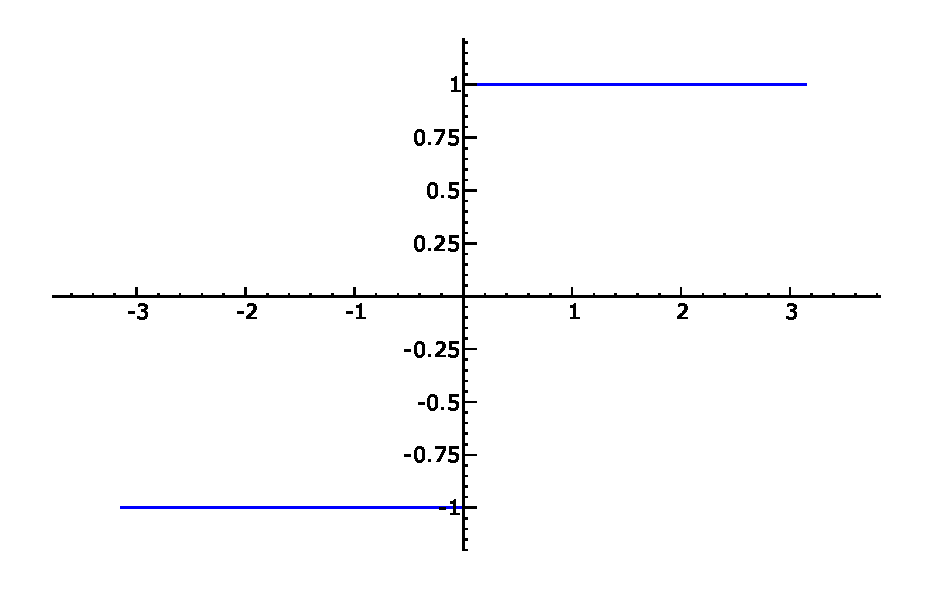
\includegraphics[width=\textwidth]{$HOME/book/fourier/img/9April2008stepFunction.eps}
  \end{center} 
  \caption[Step Function]{Step function that we make
    periodic.}
  \label{fig:9April2008:stepFunction}
\end{figure}
We would like to compute the Fourier series of this step
function, but observe that
\begin{equation}
\int f(\theta)d\theta = |\theta|
\end{equation}
and we previously calculated the Fourier series of this
function! Recall from Eq
\eqref{eq:2April2008:fourierSeriesAbsoluteTheta} that
\begin{equation}
|\theta| = \frac{\pi}{2} - \frac{4}{\pi}\sum^{\infty}_{n=1}\frac{\cos((2n-1)\theta)}{(2n-1)^2}.
\end{equation}
We take its derivative to find
\begin{equation}
\frac{d}{d\theta}|\theta| = \frac{4}{\pi}\sum_{n=1}\frac{\sin((2n-1)\theta)}{2n-1}
\end{equation}
and we identify it with the Fourier series of the step
function
\begin{equation}
f(\theta) = \frac{4}{\pi}\sum_{n=1}\frac{\sin((2n-1)\theta)}{2n-1}.
\end{equation}
\end{ex}

\section[Decay of Coefficients, Arbitrary Intervals]{Smoothness and Decay of Fourier Coefficients, Fourier Expansion on Arbitrary Intervals}
%%
%% 11April2008.tex
%% 
%% Made by Alex Nelson
%% Login   <alex@tomato>
%% 
%% Started on  Fri Dec 19 22:14:44 2008 Alex Nelson
%% Last update Fri Dec 19 22:14:44 2008 Alex Nelson
%%

Here is a deep concept that we will re-examine in Lie Groups
(perhaps if we get there): any periodic function can be
considered a function on a circle. (In a hand-wavy way, we
can change the period to be from $p$ to $2\pi$ by a change
of coordinates, then we've got from the Fourier Series a
linear combination of functions on the circle $\exp(inx)$
which are all linearly independent.)
\begin{defn}
Let $k\in\mathbb{N}$. A function $f:\mathbb{R}\to\mathbb{R}$
is of class $C^k$\index{$C^k$}, $f\in C^k$, if $f$ has derivatives up to
order $k$ and (in addition to the derivatives existing) they
are continuous. When we discuss \textbf{smoothness}\index{Smooth}, we are
discussing the existence of derivatives.
\end{defn}
At first it may seem useless to introduce such a definition,
but the strength in having such a system is that all
$C^{k+1}$ functions are also $C^{k}$ functions. It provides
a clear hierarchy of ``nice'' functions.\marginpar{$C^0$ are continuous functions}But also note, if a function is
continuous, then it is necessarily $C^0$. 

But let us reiterate what we have done before we
continue. Let $f$ be a $2\pi$ periodic, piecewise smooth and
continuous. This means $f\in C^0$ and $f'\in
PC(\mathbb{R})$. This means that $f(\theta)=\sum
c_{n}e^{in\theta}$ $\forall \theta$. This series \emph{converges
absolutely and uniformly}.\index{Convergence!Fourier Series} Also, the derivative of $f$ is
equal to the termwise derivatives of its Fourier series
\begin{equation}
f'(\theta) = \sum^{\infty}_{n=-\infty}inc_{n}e^{in\theta} =
\sum n(-a_{n}\sin(n\theta)+b_{n}\cos(n\theta))
\end{equation}
at $\theta$ where $f'$ is continuous. If we apply the Bessel
Inequality, we have the following inequality on $f'$:
\begin{equation}
\sum
|nc_{n}|^{2}\leq\frac{1}{2\pi}\int^{\pi}_{-\pi}|f'(\theta)|^{2}d\theta
< \infty
\end{equation}
So it follows that
\begin{equation}
nc_{n}\to 0\quad\text{as }n\to\infty
\end{equation}
Similarly we can argue that $\sum|na_{n}|^{2}$ and $\sum
|nb_{n}|^{2}$ are finite. So $na_{n}\to 0$ and $nb_{n}\to 0$
as $n\to\infty$.

So this implies $a_n, b_n\sim 1/n^k$ where $k>1$. If $f\in
C^1$ and $f''\in PC^{1}(\mathbb{R})$, then we can apply the
same result again
\begin{equation}
\sum |nc_{n}|^{2}\leq
\frac{1}{2\pi}\int^{\pi}_{-\pi}|f''(\theta)|^{2}d\theta <
\infty
\end{equation}
So $n^2c_n$, $n^2a_n$, $n^2b_n\to 0$ as $n\to\infty$. There
is a general pattern which is beginning to emerge here.

\begin{thm}
Let $f$ be $2\pi$-periodic, if $f\in C^{k-1}$ and
$f^{(k)}\in PC(\mathbb{R})$, then
\begin{equation}
\sum|c_{n}n^k|^2\leq\frac{1}{2\pi}\int^{\pi}_{-\pi}|f^{(k)}(\theta)|^{2}d\theta<\infty
\end{equation}
which implies $n^kc_n\to 0$ as $n\to\infty$. Thus
\begin{equation}
|c_n|\leq\frac{\text{(constant)}}{n^k +
  \varepsilon_{n}},\qquad\text{where }\varepsilon_{n}>0.
\end{equation}
\end{thm}
On the other hand, if we compute the Fourier coefficients of
a function and $|c_n|\leq c/|n|^{k+\alpha}$ where $c>0$,
$\alpha>0$, we may say that $f$ is $C^{k-1}$.

\subsection{Fourier Series on Arbitrary Interval}

Fourier series on an interval $[a,b]$ where $a<b$. How is
this done? Well, usually, as a rule of thumb, we don't work
all of $\mathbb{R}$ (so $-\infty<a<b<+\infty$). For
instance, the heat distribution
\begin{eqnarray*}
f(x) &= \text{temperature distribution along a rod of length
  $L$} \\
&f:[0,L]\to\mathbb{R}
\end{eqnarray*}
More generally, let $s(t)$ be a signal generated over a time
interval $[0,T]$.

The strategy is to first change variables to make the domain
from $[0,\pi]$; then we extend our (odd or even) Fourier
coefficients to make $f$ defined on $[-\pi,\pi]$. Then we
can just make it periodic to extend it to all of
$\mathbb{R}$. If one examines any Fourier expansion table,
the functions are usually defined on the interval
$[-\pi,\pi]$ (or $[0,2\pi]$). They are periodic extensions
of functions defined on $[-\pi,\pi]$ to $\mathbb{R}$. 

\begin{defn}
Let $f:[-\pi,\pi)\to\mathbb{C}$, then
  $f_{ext}:\mathbb{R}\to\mathbb{C}$ is defined by
  $f_{ext}(\theta+2\pi)=f(\theta)$ for all
  $\theta\in[-\pi,\pi]$ is the \textbf{periodic extension of
    $f$ to $\mathbb{R}$}\index{Periodic Extension}.
\end{defn}

\textbf{CAUTION:} $f_{ext}$ may be discontinuous and
nondifferentiable at $\theta=(2n-1)\pi$ where
$n\in\mathbb{Z}$. So $f_{ext}$ is continuous at
$\theta=(2n-1)\pi$ if and only if
$f(-\pi)=f(\pi^{-})$. Similarly, $f_{ext}^{(k)}((2n-1)\pi)$
exists if and only if $f^{(j)}(\pi^{-})=f^{(j)}(-\pi^{+})$
where $j=0,1,2,...,k$.

\begin{ex}
Consider $f(\theta)=\theta^2$ where
$\theta\in[-\pi,\pi)$. We have $f:[a,b]\to\mathbb{C}$, then
  we change variable
\begin{equation}
\theta = \pi\left(\frac{x-a}{b-a}\right),\qquad
0\leq\theta\leq\pi
\end{equation}
Observe what is going on, we rearrange these terms given
arbitrary $a$ and $b$ to find some change of variables from
the interval $[a,b]$ to a new interval. It is seen to be
\begin{equation}
g(\theta) = f(x) = f\left(\frac{b-a}{\pi}\theta +
a\right),\quad g:[0,\pi]\to\mathbb{C}
\end{equation}
So we can see a fairly clean and orderly scheme of how to
change the interval.
\end{ex}

\begin{defn}
Let $f:[0,\pi]\to\mathbb{C}$, then the \textbf{odd
  extension}\index{Periodic Extension!Odd Extension} of $f$ to $[-\pi,\pi]$ is
\begin{subequations}
\begin{align}
f_{odd}(-\theta) &= -f(\theta), \quad 0<\theta<\pi\\
f_{odd}(0) &= 0
\end{align}
\end{subequations}
and the \textbf{even extension}\index{Periodic Extension!Even Extension} of $f$ to $[-\pi,\pi]$ is 
\begin{equation}
f_{even}(-\theta) = f(\theta),\qquad 0\leq\theta\leq\pi
\end{equation}
(note the possible values for $\theta$ differ for even and
odd extensions).
\end{defn}

So what about the Fourier Series of Periodically Extended
functions?\index{Periodic Extension!Fourier Series} It's
fairly straightforward to find for odd extensions:
\begin{subequations}
\begin{align}
a_{n} &=
\frac{1}{\pi}\int^{\pi}_{0}f_{odd}(\theta)\cos(n\theta)d\theta
= 0\\
b_{n} &=
\frac{1}{\pi}\int^{\pi}_{0}f_{odd}(\theta)\sin(n\theta)d\theta\\
\Rightarrow \sum^{\infty}_{n=1}b_{n}\sin(n\theta) &=
\text{``Fourier Sine Series''}
\end{align}
\end{subequations}
and for even extensions:
\begin{subequations}
\begin{align}
a_{n} &=
\frac{1}{\pi}\int^{\pi}_{0}f_{even}(\theta)\cos(n\theta)d\theta\\
b_{n} &=
\frac{1}{\pi}\int^{\pi}_{0}f_{even}(\theta)\sin(n\theta)d\theta=0\\
\Rightarrow \sum^{\infty}_{n=1}a_{n}\cos(n\theta) &=
\text{``Fourier Cosine Series''}
\end{align}
\end{subequations}

\section{A Review of Vector Spaces}\index{Vector Space}
%%
%% reviewVectorSpace.tex
%% 
%% Made by Alex Nelson
%% Login   <alex@tomato>
%% 
%% Started on  Wed Dec 17 14:54:08 2008 Alex Nelson
%% Last update Wed Dec 17 14:54:08 2008 Alex Nelson
%%
%%\section{A Review of Vector Spaces}\index{Vector Space}
Remember that the real numbers (denoted as $\mathbb{R}$) and
the complex numbers (denoted as $\mathbb{C}$) are usually
the scalars we work with in linear algebra (there are other
neurotic examples that mathematicians love, but since this
is for physicists, we won't examine them). We will generally
call this set of scalars, equipped with scalar
multiplication and scalar addition, a
``\textbf{field}''\index{Scalar Field}. We
will denote a generic field of scalars as $\mathbb{F}$.

Now, a \textbf{vector space} $V$ is always given as being ``over'' a
field of scalars $\mathbb{F}$. It is equipped with only two
operations:
\begin{enumerate}\index{Vector Space!Axioms}
\item Vector Addition, $+:V\times V\to V$ which is denoted
  as $\mathbf{v}+\mathbf{w}$, where
  $\mathbf{v},\mathbf{w}\in V$,
\item Scalar Multiplication, $*:\mathbb{F}\times V\to V$,
  denoted usually by $\alpha\mathbf{v}$ for all
  $\alpha\in\mathbb{F}$ and $\mathbf{v}\in V$
\end{enumerate}
It \emph{DOES NOT} have a cross product, or a dot product,
or any other sort of fun stuff. These \emph{ARE NOT}
properties of a vector space. The \emph{ONLY} properties are
scalar multiplication and vector addition. 

We need to specify several properties of vector addition and
scalar multiplication. There are four axioms of vector
addition
\begin{enumerate}\index{Vector Space!Vector Addition}
\item Vector addition is associative: for all
  $\mathbf{u},\mathbf{v},\mbf{w}\in V$, we have
  $\mbf{u}+(\mbf{v}+\mbf{w})=(\mbf{u}+\mbf{v})+\mbf{w}$;
\item Vector Addition is commutative: for all
  $\mbf{v},\mbf{w}\in V$, we have
  $\mbf{v}+\mbf{w}=\mbf{w}+\mbf{v}$;
\item Vector addition has an identity element: there exists
  an element $\mbf{0}\in V$ (dubbed the \textbf{zero
    vector}) such that $\mbf{v}+\mbf{0}=\mbf{v}$ for all
  $\mbf{v}\in V$;
\item Vector Addition has inverse elements: For all
  $\mbf{v}\in V$ there exists an element $\mbf{w}\in V$,
  called the \textbf{additive inverse} of $\mbf{v}$, such
  that $\mbf{v}+\mbf{w}=\mbf{0}$.
\end{enumerate}
Now, it is important to note that the zero vector is
unique. Observe a short proof: suppose we have two zero
vectors $\mbf{0}$ and $\widetilde{\mbf{0}}$, then for some
$\mbf{v}$ and its additive inverse $\mbf{w}$ we have
\begin{subequations}
\begin{align}
\mbf{v}+\mbf{w} &= \mbf{0} \\
&= \widetilde{\mbf{0}} \\
\Rightarrow \mbf{0} &= \widetilde{\mbf{0}}
\end{align}
\end{subequations}
Which implies the uniqueness of the zero vector.

There are similarly four axioms of scalar multiplication:
\begin{enumerate}\index{Vector Space!Scalar Multiplication}
\item Distributivity holds forscalar multiplication over
  vector addition:
  $\alpha(\mbf{v}+\mbf{w})=\alpha\mbf{v}+\alpha\mbf{w}$ for
  all $\alpha\in\mathbb{F}$, $\mbf{v},\mbf{w}\in V$;
\item Distributivity holds for scalar multiplication over
  field addition (ie. adding two scalars and multiplying by
  their sum):
  $(\alpha+\beta)\mbf{v}=\alpha\mbf{v}+\beta\mbf{w}$ for all
  $\alpha,\beta\in\mathbb{F}$ and $\mbf{v}\in V$.
\item Scalar multipication is compatible with multipocation
  in the sense of the field of scalars:
  $\alpha(\beta\mbf{v})=(\alpha\beta)\mbf{v}$ for all
  $\alpha,\beta\in\mathbb{F}$ and $\mbf{v}\in V$.
\item Scalar multiplication has an identity element:
  $\mbf{1}\mbf{v}=\mbf{v}$ for all $\mbf{v}\in V$ and the
  multiplicative identity of $\mathbb{F}$: $\mbf{1}$. 
\end{enumerate}

%%
%% 16April2008.tex
%% 
%% Made by Alex Nelson
%% Login   <alex@tomato>
%% 
%% Started on  Sat Dec 20 09:36:45 2008 Alex Nelson
%% Last update Sat Dec 20 09:36:45 2008 Alex Nelson
%%

\subsection{Inner Products}

Now we wish to speak of certain ``extra-structure'' on top
of a vector space. What is this ``extra-structure'' of which
I speak? Well, things like the norm, the inner product,
these sort of ``extra goodies'' are the ``extra-structure''
that I am going to discuss. Let us first consider the table
of similarities between the $k$ dimensional vector space
with complex entries (i.e. a vector space over the field
$\mathbb{C}$ with $k$ dimensions denoted as $\mathbb{C}^k$
which consists of an ordered ``$k$-tuple'' consisting of $k$
components, with vector addition and scalar multiplication
defined componentwise) with the piecewise continuous
functions on $(a,b)$ (which we denote as $PC(a,b)$).

\begin{tabular}{|p{0.48\textwidth}|p{0.48\textwidth}|}
\hline 
$\mathbb{C}^{k}$ & $PC(a,b)$ \\ 
\hline
$k$ dimensional & infinite dimensional \\ \hline
$\vec{a} = (a_1,...,a_k)$ with $a_j\in\mathbb{C}$ & elements
are functions that are piecewise continuous on
$[a,b]$. \\ \hline
Addition is done componentwise \newline $\vec{a}+\vec{b}=(a_1+b_1,...,a_n+b_n)$ & The
``components'' are continuous, so we do addition
``point-wise'' \newline $f(x)+g(x)$ \\ \hline
Scalar multiplication done componentwise\newline
$\alpha\vec{a}=(\alpha a_1,...,\alpha a_k)$ & Scalar
multiplication is done in the naive way by merely
multiplying by a constant
$\alpha f(x)$ \\ \hline
\end{tabular}

Now we would like to consider the various ``extra
structure'' that we can add to a vector space, and whether
this can be generalized in the $PC(a,b)$ vector space.

\begin{tabular}{|p{0.48\textwidth}|p{0.48\textwidth}|}
\hline 
$\mathbb{C}^{k}$ & $PC(a,b)$ \\ 
\hline
We sum up the entries componentwise\newline
for the inner product\footnote{The dot product is a certain
  version of the inner product, the inner product is then
  the mathematical structure we would like to examine.}
Mathematicians use the notation\newline
$\<a,b\> = \sum^{k}_{j}a_{j}\bar{b}_{j}$\newline
but physicists use Bra-Ket notation\newline
$\<b|a\>=\<a,b\>$ is the translation between the two notations
&
We similarly sum up all the points for two functions\newline
$\<f,g\> = \int^{b}_{a}f(x)\bar{g(x)}dx$ \\ \hline
We have $\<\vec{0},\vec{u}\>=0$ for all
$\vec{u}\in\mathbb{C}^k$ &
$\<0,f\>=0$ for all $f\in PC(a,b)$. \\ \hline
\end{tabular}

Observe the consequences of defining the inner product for
$PC(a,b)$ to be
\begin{equation}
\<f,g\> = \int^{b}_{a}f(x)\overline{g(x)}dx
\end{equation}
we have linearity in the first slot\index{Inner Product!Linearity In First Slot}
\begin{equation}
\<\alpha f + \beta g, h\> = \alpha\<f,h\> + \beta\<g,h\>
\end{equation}
for arbitrary $\alpha,\beta\in\mathbb{C}$. \marginpar{Linearity in first slot}We can see this
by going back to the definition of the inner product and
plugging it in
\begin{subequations}
\begin{align}
\<\alpha f + \beta g, h\> &= \int^{b}_{a}(\alpha f(x) +
\beta g(x))\overline{h(x)}dx \\
&= \int^{b}_{a}\left(\alpha f(x)\overline{h(x)} + \beta
g(x)\overline{h(x)}\right)dx\\
&= \int^{b}_{a} \alpha f(x)\overline{h(x)}dx +
\int^{b}_{a}\beta g(x)\overline{h(x)}dx\\
&= \alpha\int^{b}_{a}f(x)\overline{h(x)}dx +
\beta\int^{b}_{a}g(x)\overline{h(x)}dx\\
&= \alpha\<f,h\> + \beta\<g,h\>.
\end{align}
\end{subequations}
All we used was the distributivity of multiplication, the
linearity of the integral (twice actually), and then we
concluded with using the definition of the inner product on
$PC(a,b)$.

There is also a similar property for the second slot, but it
is called \textbf{antilinear}\index{Inner Product!Antilinearity of Second Slot}
This sounds bizarre, but using the same song and dance we
see that
\begin{equation}
\<f,\alpha g\> = \bar{\alpha}\<f,g\>
\end{equation}
where $\bar{\alpha}$ is the complex conjugate of
$\alpha$. However, we see that
\begin{subequations}
\begin{align}
\<f,g+h\> &=
\int^{b}_{a}f(x)(\overline{g(x)}+\overline{h(x)})dx \\
&= \int^{b}_{a}(f(x)\overline{g(x)}+f(x)\overline{h(x)})dx \\
&= \int^{b}_{a}f(x)\overline{g(x)}dx+\int^{b}_{a}f(x)\overline{h(x)}dx\\
&= \<f,g\> + \<f,h\>.
\end{align}
\end{subequations}
\marginpar{Antilinearity in second slot}Thus antilinearity in the second slot can be summed up as
\begin{equation}
\<f,\alpha g + \beta h\> = \bar{\alpha}\<f,g\> +
\bar{\beta}\<f,h\>
\end{equation}
for $\alpha,\beta\in\mathbb{C}$.

The last property of the inner product of interest is its
Hermitian Symmetry\index{Inner Product!Hermitian Symmetric}. 
That is to say that we have
\begin{equation}
\<f,g\> = \<g,f\>^{*}
\end{equation}
which is shorthand for
\begin{equation}
\<g,f\>^{*} = \overline{\<g,f\>}.
\end{equation}
For finite dimensional vector spaces, we need to also take
the transpose. One of the peculiarities of the infinite
dimensional vector spaces like $PC(a,b)$ is that we don't
need (or even have well defined) a transpose operation.

\subsection{Induced Norm}

Let us review the case of the properties of the norm for
finite dimensional vector spaces $V$ over $\mathbb{C}$. Once
we have an inner product, we can define (invent, or
``induce'') a norm\index{Norm!Induced from Inner Product}
\begin{equation}
\|n\| = \sqrt{\<n,n\>}.
\end{equation}
So in $\mathbb{C}^k$, this would be
\begin{equation}
\|\vec{a}\| = \sqrt{\sum^{k}_{j=1}|a_{j}|^{2}}
\end{equation}
but in $PC(a,b)$ we have
\begin{equation}
\|f\| = \left(\int^{b}_{a}|f(x)|^{2}dx\right)^{1/2}
\end{equation}
So the question arises: what are the properties of the norm?

The norm has the property of
homogeneity\index{Norm!Homogeneity} which means
\begin{equation}
\|\alpha\vec{u}\| = |\alpha|\|\vec{u}\|
\end{equation}
for all $\alpha\in\mathbb{C}$ and $\vec{u}\in V$.

Additionally, there is the property of
positivity\index{Norm!Positivity}
\begin{equation}
\|\vec{a}\|=0\iff \vec{a}=\vec{0},\quad\text{and
}\|\vec{a}\|>0\quad\forall\vec{a}\neq\vec{0}
\end{equation}
or in other words, the norm of a vector is zero if and only
if it is the zero vector. Otherwise, the norm of a vector is positive.

Now, the condition of positivity is not strictly true for
the vector space $PC(a,b)$. Consider, working on $PC(0,1)$,
the function
\begin{equation}
f(x) = \begin{cases} x & \text{if }x=(1/4),(1/2),(3/4) \\
0 & \text{otherwise}
\end{cases}
\end{equation}
Then we see that
\begin{subequations}
\begin{align}
\|f\|^2 &= \int^{1/4}_{0}(0)dx + \int^{1/2}_{1/4}(0)dx +
\int^{3/4}_{1/2}(0)dx + \int^{1}_{3/4}(0)dx \\
&= 0
\end{align}
\end{subequations}
but $f(x)\neq 0$. 

The convention we use is that in $PC(a,b)$ two functions are
considered to be equal $f(x)=g(x)$ if they agree except at
finitely many points. The motivation for this is, in finite
dimensional vector space, if
\begin{equation}
\vec{u}=\vec{v}
\end{equation}
then
\begin{equation}
\vec{u}-\vec{v}=\vec{0}\Rightarrow\|\vec{u}-\vec{v}\|=0.
\end{equation}
So, this would mean that the two are equal. If there are
only a finite number of points where $f(x)$ disagrees with
$g(x)$, then the norm of the difference would vanish. So by
the above scratch work, it would imply that $f(x)=g(x)$.

\begin{lem}
For any $u,v\in V$ (of arbitrary dimension), then
\begin{equation}
\|u+v\|^2 = \|u\|^2 + \|v\|^2 + 2\re\left(\<u,v\>\right).
\end{equation}
\end{lem}
\begin{proof}
It trivially follows from the Hermitian symmetry of the
inner product (that is no proof, it should be
noted). Observe that
\begin{subequations}
\begin{align}
\|u+v\|^2 &= \<u+v,u+v\> \\
&= \<u,v\>+\<v,u\>+\<u,u\>+\<v,v\> \\
&=\re\left(\<u,v\>\right)+\|u\|^2+\|v\|^2
\end{align}
\end{subequations}
which is an explicit calculation.
\end{proof}\marginpar{Cauchy-Schwarz Inequality}\index{Norm!Cauchy-Schwarz Inequality}\index{Cauchy-Schwarz Inequlity|see{Norm}}
\begin{lem}{(Cauchy-Schwarz Inequality)}
Let $u,v\in V$ then
\begin{equation}
|\<u,v\>|\leq\|u\|\|v\|
\end{equation}
and it is an equality if and only if $u=\alpha v$ where
$\alpha\in\mathbb{C}$.
\end{lem}
\begin{proof}
For any real constant $t\in\mathbb{R}$,
\begin{subequations}
\begin{align}
0&\leq\|u+tv\|^2 \\
&\leq\|u\|^2+|t|^2\|v\|^2 + 2t\re\left(\<u,v\>\right)
\end{align}
\end{subequations}
We can assume without loss of generality that $\|v\|\neq0$
(otherwise the inequality holds trivially, a sixth grader
could show it). We can form a quadratic equation in $t$
\begin{equation}
0 \leq q(t) = \frac{\|u\|^2}{\|v\|^2} +
2\frac{\re(\<u,v\>)}{\|v\|^2}t + t^2
\end{equation}
We see that $q(t)$ is quadratic, so it has a minimum
somewhere (since its coefficients are all positive). We take
its derivative and set it to zero:
\begin{equation}
q'(t) = 2\left(\frac{\re(\<u,v\>)}{\|v\|^2} + t\right)
\end{equation}
We see when setting this to be zero that the minimum occurs when
\begin{equation}
t = -\frac{\re(\<u,v\>)}{\|v\|^2}.
\end{equation}
We plug this value of $t$ back into $q(t)$ to find
\begin{equation}\label{eq:16April2008:stepInProofThatNeedsCitation}
0\leq q\left( -\frac{\re(\<u,v\>)}{\|v\|^2}\right) = \|u\|^2 - \frac{[\re(\<u,v\>)]^2}{\|v\|^2}
\end{equation}
Without loss of generality, we may assume that
$\<u,v\>\in\mathbb{R}$. Suppose it's really complex, then we
can write it in polar form as
\begin{equation}
\<u,v\> = re^{i\theta}
\end{equation}
for $r,\theta\in\mathbb{R}$ such that $r>0$ and
$0\leq\theta<2\pi$. Then we find that
\begin{equation}
|\<u,v\>|=r
\end{equation}
which is basic complex analysis. Thus plugging this into Eq
\eqref{eq:16April2008:stepInProofThatNeedsCitation} we find
that
\begin{equation}
0\leq \|u\|^2\|v\|^2 - |\<u,v\>|^2
\end{equation}
which implies
\begin{equation}
|\<u,v\>|^2\leq\|u\|^2\|v\|^2
\end{equation}
which is precisely the inequality!
\end{proof}

\begin{lem}{(Triangle Inequality)}
Let $u,v\in V$, then
\begin{equation}
\|u\| + \|v\|\geq \|u+v\|
\end{equation}
and it is equal if $u=tv$ where $t\in\mathbb{R}$.
\end{lem}
\begin{defn}
Two vectors $u,v\in V$ are said to be \textbf{orthogonal}\index{Orthogonal!Vectors}
if $\<u,v\>=0$.
\end{defn}
\begin{lem}{(Pythagorean Theorem)}
Let $u_1,\ldots,u_n$ be mutually orthogonal vectors, then
\begin{equation}
\|u_1+\cdots+u_n\|^2 = \|u_1\|^2 + \cdots + \|u_n\|^2.
\end{equation}
\end{lem}
Now, we can think of the Fourier series of $f\in PC(a,b)$ as
a sort of expansion with respect to a given basis.

We know that $\{e^{in\theta}\}$ forms an orthogonal basis
for all $n\in\mathbb{Z}$. Observe that
\begin{equation}
\<\exp(in\theta),\exp(in\theta)\> =
\int^{\pi}_{-\pi}e^{in\theta}e^{-in\theta}d\theta = 2\pi
\end{equation}
and 
\begin{equation}
\<\exp(i(n+m)\theta),\exp(in\theta)\> =
\int^{\pi}_{-\pi}e^{im\theta}d\theta =
\frac{1}{im}\left(e^{im\pi}-e^{-im\pi}\right) = 0.
\end{equation}
So to form an orthonormal basis, we need to use the basis
$\{\exp(in\theta)/\sqrt{2\pi}\}$ for all $n\in\mathbb{Z}$.

So wait, why do we care so much about a basis? A vector is a
vector is a vector, right? Well, no, it's time to review why
basis vectors matter.

\subsection{Basis Vectors Matter}

In general, let $V$ be a vector space over
$\mathbb{C}$. Given $n$ vectors $v_1,...,v_n\in V$, we have
this set of all possible linear combinations of these
vectors called the \textbf{linear space}\index{Linear Span}
\begin{equation}
\operatorname{span}(v_1,...,v_n) =
\{a_1v_1+\cdots+a_nv_n:\forall a_1,...,a_n\in\mathbb{C}\}.
\end{equation}
Now, we can call a given collection of vectors $v_1,...,v_n$
\textbf{linearly independent} if the only scalars
$a_1,...,a_n\in\mathbb{C}$ that satisfy
\begin{equation}
a_1v_1 + \cdots + a_nv_n = 0
\end{equation}
are $a_1=\cdots=a_n=0$. This means that we cannot write any
single vector in terms of a linear combination of the other
$n-1$ vectors.

It would be lovely if we could find some collection of
linearly independent vectors whose span is equal to the
entire vector space $V$, wouldn't it? (Yes, it would.) There
is a special name we give to such collection of vectors, we
call the set a \textbf{basis}\index{Basis} and the vectors
are called (appropriately enough) \textbf{basis vectors}.

There is also a way to write any given vector as a linear
combination of a given basis. What we do is ``project'' the
given vector $x$ onto the basis vector $v_j$, which is some
scalar $\<x,v_j\>$ and then multiply the basis vector by
this quantity. So we end up with a sum
\begin{equation}
x = \sum_{j}\<x,v_j\>v_j.
\end{equation}
Let us consider a few examples.

\begin{ex}
Consider the vector space $\mathbb{R}^2$ over the scalar
field $\mathbb{R}$ with the usual dot produt. Let $e_1 =
(1,1)/\sqrt{2}$, $e_2=(1,-1)/\sqrt{2}$ be an orthonormal
basis (we see this because the dot product of a given basis
vector with itself is 1, but dot them to each other results in
0). Let $x=(3,7)$. Then we can write it as a linear
combination of the basis
\begin{equation}
x = \<x,e_1\>e_1 + \<x,e_2\>e_2
\end{equation}
Observe
\begin{equation}
\<x,e_1\> = (3+7)/\sqrt{2}=5\sqrt{2},\qquad\text{and }\<x,e_2\>=(3-7)/\sqrt{2}=-2\sqrt{2}
\end{equation}
thus
\begin{equation}
x = (5\sqrt{2})e_1 + (-2\sqrt{2})e_2 = (5e_1-2e_2)\sqrt{2}
\end{equation}
which concludes this example. If one doesn't believe it,
just plug it all back in
\begin{equation}
(5e_1-2e_2)\sqrt{2} = (5,5)+(-2,2) = (3,7).
\end{equation}
Woah, that's exactly $x$!
\end{ex}

\begin{rmk}
If we have a basis that is not composed of unit vectors, we
have to make them unit vectors \emph{BEFORE} trying to
expand a given vector in terms of them.
\end{rmk}

\begin{rmk}
The Fourier series is just an expansion in the basis
$\{\exp(in\theta)\}$, and it is normalized silently by
making the cofficients be
\begin{equation}
c_n =
\frac{1}{2\pi}\int^{\pi}_{-\pi}f(\theta)e^{-in\theta}d\theta
\end{equation}
The basis is normalized as $\exp(in\theta)/\sqrt{2\pi}$ but
then when we take the dot product of the new coefficient
\begin{equation}
\widetilde{c}_n =
\int^{\pi}_{-\pi}f(\theta)\frac{e^{-in\theta}}{\sqrt{2\pi}}d\theta
\end{equation}
and there is an extra factor of $1/\sqrt{2\pi}$ in the basis
vectors in the expansion, which yields the series being
\begin{equation}
f(\theta) =
\sum^{\infty}_{n=-\infty}\frac{1}{2\pi}e^{in\theta}\int^{\pi}_{-\pi}f(\theta)e^{-in\theta}d\theta
\end{equation}
which is precisely what we have with our original Fourier
coefficients and our original basis.
\end{rmk}

\section{$L^{2}$ spaces}
%%
%% 18April2008.tex
%% 
%% Made by Alex Nelson
%% Login   <alex@tomato>
%% 
%% Started on  Sat Dec 20 15:23:28 2008 Alex Nelson
%% Last update Sat Dec 20 15:23:28 2008 Alex Nelson
%%
%% The topics of this file are really just two thing: 1) the
%% normed vector space $L^{2}(a,b)$, its definition and some
%% prospects; 2) a look at $\{\exp(inx)/\sqrt{2\pi}\}$ is an
%% orthonormal basis in $\mathbb{R}^2\cong\mathbb{C}$.

Before beginning just a few definitions on the various types
of convergences.

\begin{defn}
Suppose $\{f_n\}$ is a sequence of functions in $L^2(a,b)$.
\begin{enumerate}
\item We say that $f_n$ converges to $f$ \textbf{pointwise}\index{Convergence!Pointwise}
if for each $x\in[a,b]$,
\begin{equation}
f_{n}(x)\to f(x)\text{ as }n\to\infty
\end{equation}
(.e. $|f_n(x)-f(x)|\to0$ as $n\to\infty$). This means for
any $\varepsilon>0$ and any $x\in[a,b]$ there is an integers
$N_{\varepsilon,x}>0$ which depends on $\varepsilon$ and $x$
such that
\begin{equation}
|f_{n}(x)-f(x)|<\varepsilon\quad\text{for all }n>N_{\varepsilon,x}
\end{equation}
\item We say that $f_n$ converges to $f$ \textbf{uniformly}\index{Convergence!Uniform}
if
\begin{equation}
\sup_{a\leq x\leq b}|f_{n}(x)-f(x)|\to0\text{ as }n\to\infty
\end{equation}
which means for each $\varepsilon>0$ there is an integer
$N>0$ such that
\begin{equation}
|f_{n}(x)-f(x)|<\varepsilon\quad\text{for all }n>N
\end{equation}
which is a stronger condition than pointwise convergence
since $N$ depends only on the choice of $\varepsilon$.
\item We say that $f_{n}$ converges to $f$ \textbf{in norm}\index{Convergence! In Norm}
if
\begin{equation}
\|f_n-f\|\to0\quad\text{as }n\to\infty
\end{equation}
where $\|\cdot\|$ is the norm on the vector space
$L^{2}(a,b)$. By the definition of the norm this means
\begin{equation}
\int^{b}_{a}|f_n(x)-f(x)|^2dx\to 0\quad\text{as }n\to\infty
\end{equation}
\end{enumerate}
\end{defn}

\textbf{Motivation:} We know that
\begin{align*}
\<\frac{1}{\sqrt{2\pi}}e^{imx},\frac{1}{\sqrt{2\pi}}e^{inx}\>
&= \frac{1}{2\pi}\int^{\pi}_{-\pi}e^{i(m-n)x}dx\\
&= \begin{cases}1&m=n\\
0&m\neq n\end{cases}
\end{align*}
So the set $\{\exp(inx)/\sqrt{2\pi}\}^{\infty}_{-\infty}$ is
an orthonormal set. We would like to make it an orthonormal
basis.

Recall in $\mathbb{C}^k$: any set $\{u_1,\ldots,u_k\}$ that
is orthonormal forms a basis for $\mathbb{C}^k$. It has two
properties of relevance
\begin{enumerate}
\item For any $v\in\mathbb{C}^k$, $v=\sum_j
  \<v,u_j\>u_k$. In other words, any vector can be written
  as a linear combination of the vectors $u_j$, $j=1,\ldots,k$.
\item the sum $\sum_{j}\alpha_{j}u_{j}$ (for all
  $\alpha_j\in\mathbb{C}$) forms some vector in $\mathbb{C}^k$.
\end{enumerate}

We want to mirror this for our $L^{2}(a,b)$ space; however,
the second property is not true for any orthonormal set
because $PC(a,b)$ is not ``complete''. 

So we move to a bigger space, $L^{2}$\index{$L^2$}, which is
defined as the set of all functions satisfying
\begin{equation}
L^{2}(a,b) = \{ \text{$f$ on $[a,b]$ s.t. }
\int^{b}_{a}|f(x)|^{2}dx<\infty \}
\end{equation}
where we use the Lebesgue integral\index{Lebesgue Integration}\index{Integration!Lebesgue Integral}. \marginpar{Don't Stress over the Lebesgue
  integral, it really is nothing special...just integration
  done in the way taught in math 21 B, but the only time we
  run into problems is with wacky functions and bizarre
  domains (e.g. domains with only a single point).}What the hell's the
Lebesgue integral, and why do we use it? The simplest
explanation is that it's the area between the $x$-axis and
the curve (one may ask ``But isn't that a Riemann
integral?'' And that's kind of true, but one typically has
vertical rectangles in the Riemann sum, whereas one would
have e.g. vertical rectangles in the Lebesgue integral).

If $f\in PC(a,b)$ then
$\int^{b}_{a}|f(x)|^{2}dx<\infty$...so $f\in L^{2}(a,b)$. So
this implies $PC(a,b)\subset L^{2}(a,b)$. Improper Riemann
integrable functions are also in $L^{2}(a,b)$. Lebesgue
integration is, to a physics undergrad, just ``really clever
integration'' (or integration done in the usual way being
careful about infinities).

\begin{ex}
Let $f(x)=x^{-1/3}$ on $[-1,1]$. This is not piecewise
continuous on $[-1,1]$ since it blows up around $0$. But
observe
\begin{align*}
\int^{1}_{-1}|f(x)|^{2}dx &= \int^{1}_{-1}x^{-2/3}dx\\
&=\lim_{\alpha\to 0^{-}}\int^{\alpha}_{-1}x^{-2/3}dx +
\lim_{\beta\to0^{+}}\int^{1}_{\beta}x^{-2/3}dx\\
&=\lim_{\alpha\to0^{-}}(3\alpha^{1/3}+3)+\lim_{\beta\to0^{+}}(3-3\beta^{1/3})\\
&= 6
\end{align*}
So $f\in L^{2}(-1,1)$.
\end{ex}

\begin{defn}
Let $E\subset\mathbb{R}$, $E$ is \textbf{(Lebesgue) measure
  zero}\index{Lebesgue Measure Zero} if for any
$\varepsilon>0$, there exists a set of intervals
$\{I_1,\ldots\}$ of length $\ell_1$, $\ldots$ such that
\begin{equation}
E\subset\cup_{j=1}I_{j}\quad\text{and
}\sum^{\infty}_{j=1}\ell_{j}<\infty
\end{equation}
Let $\Delta>0$, then $\int^{\Delta}_{0}1dx\neq 0$. For $E$
of measure zero, $\int_{E}1dx=0$.
\end{defn}

\begin{rmk}
Some functions with no Riemann integral have Lebesgue
integral.
\end{rmk}

\begin{ex}
Let $\{r_1,\ldots\}$ be enumeration of the rational numbers,
then it has Lebesgue measure zero. Let
\begin{equation}
f(x) = \begin{cases}1&\text{if $x$ is
    irrational}\\0&\text{otherwise}\end{cases}
\end{equation}
be defined on $[0,1]$. Then $f=0$ on a set of measure
zero. THe Riemann integral of $f$ does not exist, the upper
sum of $f$ is
\begin{equation}
\sum 1 \Delta x
\end{equation}
where $\Delta x$ is the width of the intervals, and the
lower sums are
\begin{equation}
\sum 0\Delta x = 0
\end{equation}
Thus
\begin{equation}
\lim_{\Delta x\to 0}\sum 1\Delta x = \sum 0\Delta
x\Rightarrow 1=0
\end{equation}
which is known to be wrong! However, for the Lebesgue
integral
\begin{equation}
\int^{1}_{0}|f(x)|^{2}dx = 1\Rightarrow f(x)\in L^{2}(0,1).
\end{equation}
\end{ex}

\textbf{Question:} \emph{Can we extend the definition of the
  inner product $\<\cdot,\cdot\>$ from $PC(a,b)$ to
  $L^{2}(a,b)$?}''

Well, we very generally defined the inner product to be
\begin{equation}
\<f,g\> = \int^{b}_{a}f(x)\overline{g(x)}dx
\end{equation}
If $\int f(x)\overline{g(x)}dx$ exists, for all $f,g\in
L^{2}(a,b)$, then $\<\cdot,\cdot\>$ is well defined.

Let $f,g$ be two functions in $L^{2}(a,b)$. Then
\begin{equation}
|\<f,g\>|\leq \int^{b}_{a}|f(x)\overline{g(x)}|dx
\end{equation}
So $|f(x)\overline{g(x)}|\leq|f(x)||g(x)|$ we know for
$s,t\in\mathbb{R}$
\begin{equation*}
0\leq (s-t)^{2} = s^{2} + t^{2} - 2st
\end{equation*}
if and only if
\begin{equation*}
\frac{1}{2}(s^2+t^2)\geq st \quad\forall s,t\in\mathbb{R}
\end{equation*}
Since $|f(x)|$ and $|g(x)|$ are both real (even if $f(x)$
and $g(x)$ are complex, their absolute value (aka their
modulus) returns the ``radial length'' which is a real
number), we see that
\begin{equation}
\frac{1}{2}\left(|f(x)|^2 + |g(x)|^2\right)\geq|f(x)||g(x)|
\end{equation}
so
\begin{equation}
|\<f,g\>|\leq\frac{1}{2}\int |f(x)|^2 + |g(x)|^2dx<\infty.
\end{equation}
Thus we may extend the inner product $\<\cdot,\cdot\>$ from
$PC(a,b)$ to $L^{2}(a,b)$. All properties of the inner
product and the norm still hold.

Three is one more property that also holds that we have been
trying to prove.

\begin{bessel}\index{Bessel Inequality}
If $\{\phi_{n}\}^{\infty}_{n=1}$ is an orthonormal set in
$L^{2}(a,b)$, and if $f\in L^{2}(a,b)$, then
\begin{equation}
\sum^{\infty}_{n=1}|\<f,\phi_{n}\>|^{2} \leq
\|f\|^2\qquad\text{in $L^{2}(a,b)$}
\end{equation}
\end{bessel}
\begin{proof}
Let $N$ be any positive integer,
\begin{align*}
0 &\leq \|f - \sum^{N}_{n=1}\<f,\phi_n\>\phi_n\|^2\\
&=\|f\|^2 - 2\re(\<f,\sum^{N}_{1}\<f,\phi_n\>\phi_n) +
\|\sum^{N}_{n=1}\<f,\phi_{n}\>\phi_{n}\|^{2}
\end{align*}
We can expand out
\begin{align*}
\<f,\sum^{N}_{n=1}\<f,\phi_n\>\phi_n\> &= \sum^{N}_{n=1}
\<f,\<f,\phi_n\>\phi_n\>\\
&= \sum^{N}_{n=1}\overline{\<f,\phi_n\>}\<f,\phi_n\>\\
&= \sum^{N}_{n=1}|\<f,\phi_n\>|^{2}
\end{align*}
We put all this together to get
\begin{align*}
0 &\leq \|f\| - \sum^{N}_{n=1}\<f,\phi_n\>\phi_n\|^2\\
&\leq \|f\|^2 - \sum^{N}_{n=1}|\<f,\phi_n\>|^2
\end{align*}
for all $N$.
\end{proof}
\marginpar{Some intuition of distance}Now, for something completely different. Recall back in one
real dimension, we measure distance by taking the absolute
value of the difference between two numbers. We generalize
this in multiple dimensions, from the Pythagorean theorem,
to be the norm of the difference between two vectors. We
generalize this still to be the norm of the difference
between two functions for having some intuition of distance
in $L^{2}$ (i.e. for $f,g\in L^{2}(a,b)$, $\|f-g\|$ measures
the ``distance'' between $f$ and $g$), we also say that
$f_n$ converges to $f\in L^2(a,b)$ \textbf{in norm}\index{Convergence!In Norm} if
\begin{equation}
\|f_n - f\|\to 0\quad\text{as }n\to\infty.
\end{equation}

\section{Orthonormal Basis for $L^2$}
%%
%% 21April2008.tex
%% 
%% Made by Alex Nelson
%% Login   <alex@tomato>
%% 
%% Started on  Sat Dec 20 20:51:48 2008 Alex Nelson
%% Last update Sat Dec 20 20:51:48 2008 Alex Nelson
%%
%% We cover only the Criteria for orthonormal basis in
%% $L^{2}(a,b)$ in this section

\begin{defn}
Let $f_n,f\in L^{2}(a,b)$, $f_n\to f$ \textbf{converges in
  norm}\index{Convergence!In Norm}  $\|f_n-f\|\to0$ as
$n\to\infty$ if and only if
$\int^{b}_{a}|f_{n}(x)-f(x)|^2dx\to0$ as $n\to\infty$.
\end{defn}

\begin{rmk} 
If one has the norm of two functions $\|f-g\|=0$, then $f=g$
in $L^{2}(a,b)$ if and only if $f(x)=g(x)$ for $x$ (outside
of sets of measure zero) in $[a,b]$.
\end{rmk}

\begin{defn}
We say $f=g$ \textbf{almost everywhere} if $f(x)=g(x)$ for
$x\in[a,b]-E$ where $E$ is measure 0.
\end{defn}

\begin{ex}
Let
\begin{equation}
f(x) = \begin{cases} 0 & \text{if } x\in[0,1]\text{ is
    irrational}\\
1 & \text{if }x\in\mathbb{Q}\cap[0,1]\end{cases}
\end{equation}
then $f(x)=1$ almost everywhere.
\end{ex}

\begin{rmk}
The pointwise convergence and convergence in norm do not
imply each other.
\end{rmk}

\begin{thm}
If $f_n\to f$ uniformly on an interval $[a,b]$, then $f_n\to
f$ in norm.
\end{thm}
\begin{proof}
Let $M_n = \sup_{x\in[a,b]}|f_{n}(x)-f(x)|\to 0$ as
$n\to\infty$. Now
$\|f_n-f\|^2=\int^{b}_{a}|f_{n}(x)-f(x)|^{2}dx\leq\int^{b}_{a}M_{n}^{2}dx=M_{n}^{2}(b-a)$. But
$M_{n}\to 0$ so $M_{n}^{2}(b-a)\to 0$ too.
\end{proof}

\begin{defn}
A sequence $\{a_{n}\}$ in a normed vector space $V$ (i.e. a
vector space with a norm $\|\cdot\|$) is called a
\textbf{Cauchy Sequence}\index{Cauchy Sequence}\index{Sequence!Cauchy} 
if
\begin{equation}
\|a_m-a_n\|\to 0\quad \text{as }m,n\to\infty
\end{equation}
$V$ is \textbf{complete}\index{Complete Vector Space}
if\index{Vector Space!Complete} every Cauchy sequence
converges to a vector in $V$.
\end{defn}
\begin{ex}
In $\mathbb{R}$, $a_n=1/n$, then
\begin{align*}
\|a_m - a_n\| &= \left|\frac{1}{m}-\frac{1}{n}\right| \\
&= \left|\frac{n-m}{mn}\right|\to 0
\end{align*}
as $m,n\to\infty$. So $a_n$ is Cauchy and goes to zero.
\end{ex}
\index{$PC(\mathbb{R})$!Not Complete}\marginpar{$PC(a,b)$ is not complete}One can observe that $PC(a,b)$ is not complete by this
counter-example to the claim. Consider $PC(0,1)$ and let
\begin{equation}
f_{n}(x) = \begin{cases} x^{-1/4}&\text{if }x>1/n\\
0&\text{otherwise}\end{cases}
\end{equation}
If $m>n$, $f_m(x)-f_n(x)$ equals $x^{-1/4}$ when
$m^{-1}<x\leq n^{-1}$ and equals 0 otherwise, so
\begin{equation}
\|f_m - f_n\|^2 = \int^{1/n}_{1/m}x^{-1/2}dx =
2x^{1/2}|^{1/n}_{1/m} = 2(n^{-1/2}-m^{-1/2}),
\end{equation}
which tends to zero as $m,n\to\infty$. Thus the sequence
$\{f_n\}$ is Cauchy; but clearly its limit (either pointwise
or in norm) is
\begin{equation}
f(x) =\begin{cases} x^{-1/4}&\text{if }x>0\\
0\text{if }x=0\end{cases}
\end{equation}
and this function does not belong to $PC(0,1)$ because it
becomes unbounded as $x\to 0$.

However, it is worthy of note that $L^{2}(a,b)$ is not only
complete but the completion of $PC(a,b)$.

Rudin's notion of completeness~\cite{rudinPrinciplesOfMathematicalAnalysis}
\begin{thm}{(Rudin 11.42)}\index{$L^2$!Complete}
If $\{f_{n}\}\in L^{2}(a,b)$ (n=1,2,...) is a Cauchy
sequence, then there exists some function $f\in L^{2}(a,b)$
such that $\{f_{n}\}$ converges to $f \in L^{2}(a,b)$.
\end{thm}
This says,in other words, that $L^{2}(a,b)$ is a
\emph{complete} metric space.

\begin{thm}{(Rudin's Theorem 11.38)}
For all $f\in L^{2}(a,b)$, and for each $\varepsilon>0$,
there is a $(b-a)$-periodic function and infinitely smooth
$\widetilde{f}\in C^{\infty}(a,b)$ such that
$\|f-\widetilde{f}\|<\varepsilon$.
\end{thm}

\begin{thm}
If $\{\phi_n\}$ is an orthonormal set in $L^{2}(a,b)$, $f\in
L^{2}(a,b)$ the Bessel inequality states\index{Bessel Inequality}: 
\begin{equation}
\sum^{\infty}_{n=1}|\<f,\phi_n\>|^2\leq\|f\|^2.
\end{equation} 
Thus
\begin{equation}
\sum^{M}_{N}|\<f,\phi_n\>|^2\to 0\quad\text{as }M,N\to\infty. 
\end{equation}
Further 
\begin{equation}
\|\sum^{N}_1 \<f,\phi_n\>\phi_n\|^2=\sum^{N}_{n=1}|\<f,\phi_n\>|^2
\end{equation}
by the Pythagorean theorem. It suffices to show that
$\<f,\phi_n\>\phi_n$ is a Cauchys series
\begin{equation}
\|\sum^{N}_{M}\<f,\phi_n\>\phi_n\|^2\to 0.
\end{equation}
\end{thm}

\begin{lem}
If $f\in L^{2}(a,b)$, $\{\phi_{n}\}$ is an orthonormal set
in $L^{2}(a,b)$, then
\begin{equation}
\sum^{\infty}_{n=1}\<f,\phi_n\>\phi_n
\end{equation}
converges in norm; moreover
\begin{equation}
\|\sum^{\infty}_{n=1}\<f,\phi_n\>\phi_n\|\leq\|f\|.
\end{equation}
\end{lem}

\subsection{Criteria for an Orthonormal Basis in $L^{2}(a,b)$}

\begin{thm}
Let $\{\phi_n\}^{\infty}_{n=1}$ be an orthonormal set in
$L^{2}(a,b)$, the following conditions are equivalent
\begin{enumerate}
\item if $\<f,\phi_n\>=0$ for all $n\in\mathbb{Z}$, then
  $f=0$
\item for all $f\in L^{2}(a,b)$,
  $f=\sum^{\infty}_{n=1}\<f,\phi_n\>\phi_n$ (convergence in
  norm)
\item for all $f\in L^{2}(a,b)$, we have the
  \textbf{Parseval equality}\index{Parseval Equality}
\begin{equation}
\|f\|^2=\sum^{\infty}_{n=1}|\<f,\phi_n\>|^2.
\end{equation}
\end{enumerate}
\end{thm}
\begin{proof}
We'll prove that (1) implies (2), (2) implies (3), and (3)
implies (1).

\textbf{(1)$\Rightarrow$(2)} Suppose $\<f,\phi_n\>=0$ for
all $n$. Let
\begin{align*}
g &= f-\sum^{\infty}_{n=1}\<f,\phi_n\>\phi_n\\
\<g,\phi_m\> &=
\<f,\phi_m\>-\sum^{\infty}_{n=1}\<f,\phi_n\>\<\phi_n,\phi_m\>\\
&=\<f,\phi_m\>-\sum^{\infty}_{n=1}\<f,\phi_n\>\delta_{nm}\\
&=\<f,\phi_m\> - \<f,\phi_m\>\\
&=0
\end{align*}
for any $m$. Therefore $g=0$.

\textbf{(2)$\Rightarrow$(3)} Suppose for any $f$, we have
\begin{equation}
f = \sum^{\infty}_{n=1}\<f,\phi_n\>\phi_n
\end{equation}
So
\begin{align*}
\|f\|^2 &= \<f,f\> =
\|\sum^{\infty}_{n=1}\<f,\phi_n\>\phi_n\|^2\\
&=\lim_{N\to\infty}\|\sum^{N}_{n=1}\<f,\phi_n\>\phi_n\|^2\\
&=\lim_{N\to\infty}\sum^{N}_{n=1}|\<f,\phi_n\>|^2\quad\text{by Pythagorean thm}\\
&=\sum^{\infty}_{n=1}|\<f,\phi_n\>|^2.
\end{align*}

\textbf{(3)$\Rightarrow$(1)} Suppose 
\begin{equation}
\|f\|^2 = \sum^{\infty}_{n=1}|\<f,\phi_n\>|^2
\end{equation}
Suppose $\<f,\phi_n\>=0$ for all $n$. Then $\|f\|^2=0$ which
implies $f=0$ in $L^{2}(a,b)$.
\end{proof}

\begin{rmk}
In $\mathbb{C}^k$ where $\vec{v}=(v_1,...,v_k)$, then
\begin{equation}
\|\vec{v}\|^2 = \sum^{k}_{j=1}|\<v,e_j\>|^2
\end{equation}
is the discrete version of Parseval equality.
\end{rmk}

\section{More on Orthonormal Basis, Spectral Theorem}
%%
%% 23April2008.tex
%% 
%% Made by Alex Nelson
%% Login   <alex@tomato>
%% 
%% Started on  Sun Dec 21 12:44:51 2008 Alex Nelson
%% Last update Sun Dec 21 12:44:51 2008 Alex Nelson
%%
\begin{thm}
The set $\{\exp(inx)/\sqrt{2\pi}\}^{\infty}_{-\infty}$ is an
orthonormal basis in $L^{2}(-\pi,\pi)$. (Equivalently,
\begin{equation*}
\left\{\frac{1}{\sqrt{2\pi}}\right\}\cup\left\{\frac{\cos(nx)}{\sqrt{\pi}}\right\}^{\infty}_{1}\cup\left\{\frac{\sin(nx)}{\sqrt{\pi}}\right\}^{\infty}_{1}
\end{equation*}
is an orthonormal basis in $L^{2}(-\pi,\pi)$.)
\end{thm}

\begin{proof}
Fix an arbitrary $f\in L^{2}(a,b)$. Let $\psi_n(x) =
\exp(inx)/\sqrt{2\pi}$. $\alpha_n=\<f,\psi_n\>$. We want to
show that 
$$\|f-\sum^{N}_{n=-N}\alpha_{n}\psi_{n}\|\to0\text{ as
}n\to\infty$$
(Note that $\sum \alpha_n\psi_n$ is the Fourier series of
$f$).
Let $\varepsilon>0$ be given. We will show that there exists
an $N\in\mathbb{N}$ such that for all $M\geq N$ the norm
\begin{equation}
\|f-\sum^{M}_{n=-m}\alpha_n\psi_n\|<\varepsilon
\end{equation}
\begin{enumerate}
\item There is an $\widetilde{f}$ $2\pi$-periodic,
  infinitely smooth function such that
  $\|f-\widetilde{f}\|<\varepsilon/3$
\item The fourier series
  $\sum^{\infty}_{-\infty}\widetilde{\alpha}_n\psi_n\to\widetilde{f}$
  uniformly, hence it converges in norm, so there is an
  $N\in\mathbb{N}$ such that for all $M\geq N$,
  $\|\widetilde{f}-\sum^{M}_{-M}\widetilde{\alpha}_n\psi_n\|<\varepsilon/3$
\item So
\begin{align*}
\|\sum^{M}_{-M}(\widetilde{\alpha}_n-\alpha_n)\psi\|^2 &=
\sum^{M}_{-M}|\widetilde{\alpha}_n-\alpha_n\|^2\text{ (Pythagorean thm)}\\
&\leq\sum^{\infty}_{n=-\infty}|\widetilde{\alpha}_n-\alpha_n|^2\\
&\leq|\widetilde{f}-f|^2\text{ (Bessel Inequality)}
\end{align*}
\end{enumerate}
Because $\widetilde{\alpha}_n - \alpha_n = \<\widetilde{f}-f,\psi_{n}\>$.

Finally for any $M\geq N$,
\begin{align*}
\|f-\sum^{M}_{-M}\alpha_n\psi_n\| &= \|f-\widetilde{f}+\widetilde{f}-\sum^{M}_{-M}\widetilde{\alpha}_n\psi_n+\sum^{M}_{-M}\widetilde{\alpha}_n\psi_n-\sum^{M}_{-M}\alpha_n\psi_n\|\\
&\leq \|f-\widetilde{f}\| + \|\widetilde{f}-\sum^{M}_{-M}\widetilde{\alpha}_n\psi_n\|+\|\sum^{M}_{-M}(\widetilde{\alpha}_n-\alpha_n)\psi_n\|\\
&< (\varepsilon/3) + (\varepsilon/3) + (\varepsilon/3)\\
&< \varepsilon.
\end{align*}
\end{proof}

\subsection{Summary on Convergence of Fourier Series}

\begin{enumerate}
\item The series converges unifrmly and absolutely if $f$ is
  continuous and piecewise smooth.
\item The series converges pointwise and in norm if $f$ is
  piecewise continuous and piecewise smooth.
\item It converges in norm if $f\in L^{2}(a,b)$
\end{enumerate}

\begin{parseval}\index{Parseval Equality}
Let $\{\psi_n\}^{\infty}_{-\infty}$ be an orthonormal basis
in $L^{2}(a,b)$, for any $f\in L^{2}(a,b)$, then
\begin{equation}
\|f\|^2 = \sum^{\infty}_{-\infty}|\<f,\psi_n\>|^2.
\end{equation}
\end{parseval}

\subsection{Some Advanced Linear Algebra}

\begin{defn}\index{Hilbert Space}
A vector space $V$ (over some field of scalars $\mathbb{F}$)
with an inner product $\<\cdot,\cdot\>$ and an induced norm
$\|\cdot\|$ if it is complete under convergence in norm
(meaning that every series of vectors converges in norm to
some vector in $V$) is a \textbf{Hilbert Space}.
\end{defn}
\begin{ex}
Just a few examples, $L^{2}(a,b)$ is a Hilbert space,
$\mathbb{C}^k$ is a Hilbert space too, and $\mathbb{R}^n$ is
a Hilbert space as well.
\end{ex}

\begin{defn}\index{Linear Transformation|see{Linear Operator}}\index{Linear Operator}\index{Adjoint|see{Linear  Operator}}\index{Linear Operator!Adjoint}\index{Self Adjoint|see{Linear Operator}}\index{Linear Operator!Self Adjoint}\index{Linear Operator!Linear Transformation}
Let $W_1$, $W_2$ be subspaces of a Hilbert space. A
\textbf{linear transformation} $T:W_1\to W_2$ is a linear
map from $W_1$ to $W_2$. The \textbf{adjoint} of $T$ is
defined by
\begin{equation}
\<T\vec{a},\vec{b}\>=\<\vec{a},T^{\dag}\vec{b}\>
\end{equation}
And $T$ is \textbf{self-adjoint} if $T=T^{\dag}$.
\end{defn}
\begin{ex}
In $\mathbb{C}^k$, we can represent operators by square
matrices $T=[t_{ij}]$ ($i,j=1,...,k$). The adjoint is
$T^{\dag}=[\overline{t}_{ji}]$. Or if one prefers, this is the
complex conjugate transpose of the matrix. In
$\mathbb{R}^k$, self-adjoint is equivalent to being
symmetric.
\end{ex}

Now one should recall that the eigenvalues/eigenvectors of
$T$ are
\begin{equation}
T\vec{a}=\lambda\vec{a}
\end{equation}
where $\lambda$ is the eigenvalue, and $\vec{a}$ is the
eigenvector. The way to think of this is that the
eigenvectors are only ``stretched'' by the operator by a
factor of $\lambda$.

For self-adjoint operators, the eigenvalues are necessarily
real\index{Self Adjoint!Real Eigenvalues}. To see this, let
$\lambda$, $\vec{a}$ be the eigenvalue and eigenvector of a
self-adjoint operator $T$. So
\begin{align*}
\<T\vec{a},\vec{a}\> &= \<\vec{a},T\vec{a}\> \\
&= \<\lambda\vec{a},\vec{a}\>\\
&= \<\vec{a},\lambda\vec{a}\>\\
&= \bar{\lambda}\<\vec{a},\vec{a}\> =
\lambda\<\vec{a},\vec{a}\>\\
\Rightarrow \lambda &=\bar{\lambda}\\
\Rightarrow &\lambda\in\mathbb{R}
\end{align*}
\marginpar{Eigenvectors of self-adjoint operator form
  orthonormal basis}
\begin{thm}{(Spectral Theorem)}\index{Spectral Theorem}
(For the finite dimensional case, specifically
  $\mathbb{C}^k$ or $\mathbb{R}^k$) For any self-adjoint
  operator $T$, there is an orthonormal basis of
  $\mathbb{C}^k$ (or $\mathbb{R}^k$) consisting of
  eigenvectors of $T$.
\end{thm}

Now one can ask ``What the hell good is this?'' Well, to
solve $T\vec{x}=\vec{b}$ where $\vec{b}$ is a given
vector. Suppose $\{u_1,\ldots,u_k\}$ are eigenvectors of $T$
forming an orthonormal basis of $\mathbb{C}^k$ and the
corresponding eigenvalues are
$\lambda_1,\ldots,\lambda_k$. We can expand
\begin{equation}
\vec{b}=\sum^{k}_{j=1}\beta_{j}\vec{u_{j}}
\end{equation}
where $\beta_{j}=\<\vec{b},\vec{u}_j\>$. Let $x_j =
\<\vec{x},\vec{u}_j\>$ then $\vec{x}=\sum
x_{j}\vec{u}_{j}$. Then just by associating each eigenvector
to each eigenvector, we have $x_j=\beta_j$.

\section{The Regular Sturm-Liouville Problem}
%%
%% 25April2008.tex
%% 
%% Made by Alex Nelson
%% Login   <alex@tomato>
%% 
%% Started on  Sun Dec 21 12:40:34 2008 Alex Nelson
%% Last update Sun Dec 21 12:40:34 2008 Alex Nelson
%%
%% We are going to start investigating the regular
%% Sturm-Liouville problem

Let us first consider an example of a regular
Sturm-Liouville problem:
\begin{ex}
Heat diffusion through an inhomogeneous thin rod is
described by
\begin{equation}
\omega(x)\partial_{t}u(x,t) =
\partial_{x}[r(x)\partial_{x}u(x,t)] + p(x)u(x,t)
\end{equation}
with non-uniform material properties, where $r(x)$ is the
speed of propagation of heat, $p(x)$ is the source of heat
at the point $x$, but specifically we require $r(x)$ and
$\omega(x)$ be positive, and $u(x,t)$ is the temperature at
point $x$ and time $t$.
\end{ex}

We can solve this using the seperation of
variables\index{Seperation of Variables!Regular Sturm-Liouville Problem}
so we have $u(x,t)=X(x)T(t)$ and plug this back into the
equation to find
\begin{equation}
\omega(x)X(x)T'(t)=T(t)\partial_{x}[r(x)X'(x)]+p(x)X(x)T(t)
\end{equation}
we divide both sides by $\omega(x)X(x)T(t)$ and set it equal
to some constant $-\lambda$:
\begin{equation}
\frac{T'(t)}{T(t)} = \frac{\partial_{x}[r(x)X'(x)]}{\omega(x)X(x)}+\frac{p(x)}{X(x)}=-\lambda.
\end{equation}
We get two equations
\begin{equation}
T'+\lambda T=0\Rightarrow T(t)=T_{0}e^{-\lambda t}
\end{equation}
where $T_{0}$ is a constant dependent on the initial
conditions, and
\begin{equation}\label{eq:25April2008:sturmLiouville}
\partial_{x}[r(x)X'(x)]+p(x)X(x)+\lambda\omega(x)X(x)=0.
\end{equation}
Solving this equation is equivalent to solving the
Sturm-Liouville problem. Similarly, if we try to solve the
wave equation we get to boil it down to the same problem.

\begin{defn}\index{Differential Operator!Linear}
Let $L$ be a map
\begin{equation*}
L: C^{2}(a,b)\to L^{2}(a,b)
\end{equation*}
be a \textbf{linear differential operator} given by
\begin{align*}
L(f) &= [rf']' + pf\\
&= rf''+r'f' + pf
\end{align*}
where $r(x)$, $r'(x)$, $p(x)$ are all continuous and
real-valued on $[a,b]$, and $r(x)>0$ on $[a,b]$.
\end{defn}

\begin{rmk}
From \eqref{eq:25April2008:sturmLiouville} it is really
equivalent to
\begin{equation}
L(f) + \lambda\omega(x)f(x)=0
\end{equation}
We can verify that $L$ is linear, or in other words
\begin{equation}
L(c_1f+c_2g) = c_1L(f)+c_2L(g)
\end{equation}
where $c_1,c_2$ are real constants, $f,g\in L^{2}(a,b)$. So
if $f,g$ satisfy the equation, then so does $c_1f+c_2g$.
\end{rmk}
So really we have $L(f)=-\lambda\omega(x)f(x)$. This looks
remarkably like an eigenvalue problem from Linear Algebra
(ahem hint hint, wink wink, nudge nudge). If we can
show that $L$ is adjoint, then we can show that the
eigenfunctions $f$ form an orthonormal basis.

\textbf{Question:} What is the adjoint of $L$? To find out
we need to find what $\<L(f),g\>$ is, and see what
$\<f,L(g)\>$ is.

Let $f,g\in C^{2}(a,b)$, then
\begin{subequations}
\begin{align}
\<L(f),g\> &= \int^{b}_{a}\left(\partial_{x}[r(x)f'(x)]+p(x)f(x)\right)\overline{g(x)}dx\\
&=\int^{b}_{a}\partial_{x}[r(x)f'(x)]\overline{g(x)}dx + \int^{b}_{a}p(x)f(x)\overline{g(x)}dx
\end{align}
\end{subequations}
Now we can integrate by parts to find
\begin{align}
\int^{b}_{a}\partial{x}[r(x)f'(x)]\overline{g(x)}dx&=r(x)f'(x)g(x)|^{b}_{a}
- \int^{b}_{a}r(x)f'(x)\overline{g'(x)}dx
\end{align}
So we can put this back in to find
\begin{align}
\<L(f),g\> &= r(x)f'(x)g(x)|^{b}_{a}-\int^{b}_{a}r(x)f'(x)\overline{g'(x)}dx+\int^{b}_{a}p(x)f(x)\overline{g(x)}dx
\end{align}
By integration by parts again we find
\begin{multline}
 r(x)f'(x)\overline{g(x)}|^{b}_{a}-\int^{b}_{a}r(x)f'(x)\overline{g'(x)}dx+\int^{b}_{a}p(x)f(x)\overline{g(x)}dx\\
=r(x)f'(x)\overline{g(x)}|^{b}_{a}-r(x)\overline{g'(x)}f(x)|^{b}_{a}-\int^{b}_{a}[r(x)\overline{g'(x)}]'f(x)dx+\int^{b}_{a}p(x)f(x)\overline{g(x)}dx
\end{multline}
We can clean this up a little to find that
\begin{equation}
\<L(f),g\> =
\int^{b}_{a}f(x)\left(\partial_{x}[r(x)\overline{g'(x)}]+g(x)\overline{g(x)}\right)dx+\underbracket{\left[r(x)f'(x)\overline{g(x)}-r(x)f(x)\overline{g'(x)}\right]}_{\text{boundary terms!}}
\end{equation}
We can write now
\begin{equation}
\<L(f),g\> =
\int^{b}_{a}f(x)\overline{\left(\partial_{x}[r(x)\overline{g'(x)}]+g(x)\overline{g(x)}\right)}dx+\text{bdry terms}
\end{equation}
where ``bdry terms'' are the boundary terms, or more simply
\begin{equation}
\<L(f),g\>=\<f,L(g)\>+\text{bdry terms}.
\end{equation}

\begin{defn}\index{Formally Self Adjoint}\index{Self Adjoint!Formally Self Adjoint}\index{Lagrange Identity!Self Adjoint Linear Differential Operator}\index{Linear Differential Operator!Lagrange Identity}
$L$ is called \textbf{formally self-adjoint} because 
\begin{equation}
\<L(f),g\>=\<f,L(g)\>+\text{boundary terms}
\end{equation}
this is sometimes called the ``Lagrange identity''.
\end{defn}

\begin{rmk}
If the boundary conditions make
\begin{equation}
[r(x)(f'(x)\overline{g(x)}-f(x)\overline{g'(x)})]^{b}_{a}=0
\end{equation}
then $L$ is self-adjoint. Such boundary conditions we call
self-adjoint boundary conditions (we will formally define it
below).
\end{rmk}

If we expand this out we find
\begin{equation}
[r(f'\bar{g}-f\bar{g}')]^{b}_{a} = r(b)(f'(b)\bar{g}(b)-f(b)\bar{g}(b)') - r(a)(f'(a)\bar{g}(a)-f(a)\bar{g}(a)')
\end{equation}
This gives us a set of two boundary conditions
\begin{align*}
B_{1}(f)&=\alpha_1f(a)+\alpha_2f'(a)+\beta_1f(b)+\beta_2f'(b)=0\\
B_{2}(f)&=\alpha_3f(a)+\alpha_4f'(a)+\beta_3f(b)+\beta_4f'(b)=0
\end{align*}
where the $\alpha$'s and $\beta$'s are constants.

\begin{defn}\index{Self Adjoint!Boundary Conditions}\index{Boundary Conditions!Self Adjoint}
The boundary conditions $B_1$, $B_2$ are called
\textbf{self-adjoint} with respect to the operator $L$ if
\begin{equation}
[r(x)(f'(x)\overline{g(x)}-f(x)\overline{g'(x)})]^{b}_{a}=0
\end{equation}
for $f,g$ satisfy $B_{1}(f)=0$, $B_{2}(f)=0$, $B_{1}(g)=0$, $B_{2}(g)=0$.
\end{defn}
\begin{ex}
There are several famous boundary conditions used all the
time:
\begin{enumerate}
\item\index{Boundary Conditions!Dirichlet}\index{Dirichlet Boundary Conditions} The
Dirichlet boundary conditions $f(a)=f(b)=0$;
\item\index{Boundary Conditions!Neumann}\index{Neumann Boundary Conditions} The
Neumann boundary conditions $f'(a)=f'(b)=0$;
\item\index{Boundary Conditions!Periodic}\index{Periodic Boundary Conditions} The
periodic boundary conditions $f(a)=f(b)$ and $f'(a)=f'(b)$.
\end{enumerate}
\end{ex}
\begin{defn}{(Regular Sturm Liouville Problem)}\index{Sturm-Liouville!Regular Problem}
Find all solutions of the boundary value problem
\begin{align*}
L(f) + \lambda\omega(x)f(x) &= 0\\
B_{1}(f)=0,\, B_{2}(f)&=0
\end{align*}
where $\lambda$ is an arbitrary constant and
\begin{enumerate}[i)]
\item $L(f)=[rf']'+pf$ where $r(x)$, $r'(x)$, $p(x)$ are
  real and continuous on $[a,b]$, and $r(x)>0$ on $[a,b]$.
\item $B_{1}(f)=B_{2}(f)=0$ are self-adjoint with respect to
  $L$
\item $\omega(x)$ is positive and continuous on $[a,b]$.
\end{enumerate}
\end{defn}
\begin{rmk}\index{Wave Equation!From Regular Sturm-Liouville Problem}
If $r(x)=1$ and $p(x)=0$ and $\omega(x)=1$, then we get
\begin{equation}
f''(x)+\lambda f(x)=0
\end{equation}
or in other words, we have the wave equation on an elastic string.
\end{rmk}
\begin{defn}\index{Eigenvalue}\index{Eigenfunction}
For $\phi$ a solution of Sturm-Liouville problem
corresponding to some constant $\lambda$, with
$\phi\neq0$m we call $\phi$ the \textbf{eigenvector} (or
more often \textbf{eigenfunction}) corresponding to the
\textbf{eigenvalue} $\lambda$
\end{defn}
Note this definition is because
\begin{equation*}
L(f)=-\omega(x)\lambda
f(x)\Rightarrow\frac{1}{\omega(x)}L(f)=-\lambda f(x)
\end{equation*}
so $\lambda$ is an eigenvalue of the linear operator
$M(f)=L(f)/\omega(x)$ and eigenfunction $f(x)$.
\begin{defn}\index{$L^{2}$!Weighted Space}\index{Weighted $L^{2}$-Space}
Suppose that $\omega(x)$ is integrable on $[a,b]$ and
$\omega(x)>0$ almost everywhere on $[a,b]$, then the
\textbf{weighted $L^{2}$-Space} is defined as the set
\begin{equation}
L^{2}_{\omega}(a,b) = \{ f: \int^{b}_{a}|f(x)|^2\omega(x)dx < \infty\}
\end{equation}
\end{defn}

\section{Properties of Weighted Inner Products}
%%
%% 28April2008.tex
%% 
%% Made by Alex Nelson
%% Login   <alex@tomato>
%% 
%% Started on  Sat Dec 20 17:48:34 2008 Alex Nelson
%% Last update Sat Dec 20 17:48:34 2008 Alex Nelson
%%
%% This section just covers two things: 1) weighted
%% $L^{2}_{\omega}(a,b)$ space; 2) eigenvalues,
%% eigenfunctions of regular Sturm-Liouville problem

Recall we just introduced $L^{2}_{\omega}(a,b) = \{
f:(a,b)\to\mathbb{R} |
\int^{b}_{a}|f(x)|^{2}\omega(x)dx<\infty\}$. For us, in
practice, we'll often have $\omega(x)>0$ and it's continuous
on $[a,b]$. We have weighted inner products and weighted
norms on $L^{2}_{\omega}(a,b)$ is defined as follows:
\begin{eqnarray}
\<f,g\>_{\omega} &=& \int^{b}_{a}f(x)\overline{g(x)}\omega(x)dx\\
\|f\|_{\omega} &=& \sqrt{\<f,f\>_{\omega}} = \left(\int^{b}_{a}|f(x)|^{2}\omega(x)dx\right)^{1/2}
\end{eqnarray}

Let demonstrate the weighted inner product\index{Weighted Inner Product}\index{Inner Product!Weighted} 
and weighted norm\index{Norm!Weighted Norm}\index{Weighted Norm}
satisfy the fundamental properties of the inner product and
norm (respectively).
\begin{enumerate}[(i)]
\item $\<f,0\>_{\omega}=0$, this is trivial (it really is,
  unlike all those other times I said something was trivial)
\item Linear in the first slot \marginpar{Linearity in First Slot}
\begin{align*}
\<\alpha f+\beta g,h\>_{\omega} &= \int^{b}_{a} (\alpha f(x)+\beta g(x))\overline{h(x)}\omega(x)dx\\
&=\int^{b}_{a} \alpha f(x)\overline{h(x)}\omega(x)dx +
\int^{b}_{a} \beta g(x)\overline{h(x)}\omega(x)dx\\
&= \alpha\<f,g\>_{\omega} + \beta\<g,h\>_{\omega}
\end{align*}
\item Antilinear in the second slot \marginpar{Antilinear in Second Slot} \begin{align*}
\<f,\alpha g+\beta h\>_{\omega} &=
\int^{b}_{a}f(x)\overline{[\alpha g(x)+\beta h(x)]}\omega(x)dx\\
&=\int^{b}_{a} f(x)\overline{\alpha h(x)}\omega(x)dx +
\int^{b}_{a} g(x)\overline{\beta h(x)}\omega(x)dx\\
&=\bar{\alpha}\<f,g\>_{\omega} + \bar{\beta}\<f,g\>_{\omega}
\end{align*}
\item Hermitian symmetric
\begin{align*}
\<f,g\>_{\omega} &=\int^{b}_{a}f(x)\overline{g(x)}\omega(x)dx\\
&=\overline{\int^{b}_{a}\overline{f(x)}g(x)\omega{x}dx},\qquad\omega:\mathbb{C}\to\mathbb{R}\\
&=\overline{\<g,f\>}_{\omega}
\end{align*}
\end{enumerate}

Those are the fundamental properties of the inner product,
so let us now consider the fundamental properties of the norm.

\begin{enumerate}[(a)]
\item{(Homogeneity)} $\|\alpha f\|_{\omega} =
  |\alpha|\|f\|_{\omega}$ (this is trivial).
\item{(Positivity)} $\|f\|_{\omega}\geq 0$ and
  $\|f\|_{\omega}=0$ if and only if $f=0$.
\end{enumerate}
Observe
\begin{align}
\|f\|^{2}_{\omega} =
\int^{b}_{a}&\underbracket[0.5pt]{|f(x)|^{2}\omega(x)}dx\\
&\text{always positive }\Rightarrow\text{ nonzero integral}\nonumber
\end{align}
If $\omega(x)=0$ on a small interval from
$[\alpha,\beta]\subset[a,b]$, then if $f(x)\neq0$ on
$f[\alpha,\beta]$ and $f(x)=0$ otherwise, but the norm
vanishes
\begin{equation}
\|f\|_{\omega} = \int^{b}_{a}|f(x)|^{2}\omega(x)dx = \int^{\beta}_{\alpha}|f(x)|^{2}\omega(x)dx=0.
\end{equation}
So
\begin{equation}
\omega(x)>0\qquad\forall x\in[a,b]
\end{equation}
is needed for the positivity of the norm. Therefore all
properties of the norm also hold. 

\begin{rmk}
The weighted inner product
\begin{equation}
\<f,g\>_{\omega} = \int^{b}_{a}f(x)\overline{g(x)}\omega(x)dx
\end{equation}
can be translated into the standard inner product
\begin{equation}
\<f\omega,g\>=\<f,\omega g\>=\<f,g\>_{\omega}
\end{equation}
because $\omega$ is real valued,
i.e. $\overline{\omega(x)}=\omega(x)$ for all
$x\in[a,b]$. We see that
\begin{equation}
0<m=\min_{x\in[a,b]}\omega(x)\leq\omega(x)\leq M=\max_{x\in[a,b]}\omega(x)
\end{equation}
which implies
\begin{equation}
0<m|f(x)|^2\leq\omega(x)|f(x)|^{2}\leq M|f(x)|^2
\end{equation}
and
\begin{align}
\overbracket[0.5pt]{\hphantom{m\int^{b}_{a}|f(x)|^{2}dx\leq\int^{b}_{a}|f(x)|^{2}\omega(x)dx}}^{\text{if $f\in L^{2}_{\omega}$, then the $L^2$ norm is bounded by this}} \hphantom{\leq M\int^{b}_{a}|f(x)|^{2}dx}\nonumber\\
m\int^{b}_{a}|f(x)|^{2}dx\leq\int^{b}_{a}|f(x)|^{2}\omega(x)dx\leq M\int^{b}_{a}|f(x)|^{2}dx\\
\hphantom{m\int^{b}_{a}|f(x)|^{2}dx}\underbracket[0.5pt]{\hphantom{\int^{b}_{a}|f(x)|^{2}\omega(x)dx\leq M\int^{b}_{a}|f(x)|^{2}dx}}_{\text{if $f\in L^{2}_{\omega}$, then the norm is finite}}\nonumber
\end{align}
Thus $L^{2}_{\omega}(a,b) = L^{2}(a,b)$. In fact, if
$\{\phi_{n}\}^{\infty}_{1}$ is an orthonormal basis for
$L^{2}(a,b)$, then we may obtain a basis
$\{\psi_{n}\}^{\infty}_{1}$ for $L^{2}_{\omega}(a,b)$ where 
\begin{equation}
\psi_{n}(x) = \frac{1}{\sqrt{\omega(x)}}\phi_{n}(x).
\end{equation}
The other way holds too, given $\psi_{n}$ we find
\begin{equation}
\phi_{n} = \sqrt{\omega(x)}\psi_{n}
\end{equation}
as an orthonormal basis for $L^{2}$.
\end{rmk}
We can use this to solve the regular Sturm-Liouville
problem. We want to prove the Sturm-Liouville problme has
its eigenfunctions form an orthonormal basis of
$L^{2}(a,b)$. Recall the linear operator we're working with is
\begin{align}
L(f)+\lambda\underbracket[0.5pt]{\omega(x)}&f(x)=[r(x)f'(x)]'+p(x)f(x)+\lambda\underbracket[0.5pt]{\omega(x)}f(x)=0\\
 &\!\!\!\!\!\!\!\uparrow \qquad\qquad\qquad\qquad\qquad\qquad\qquad\qquad\quad \!\!\!\!\uparrow \nonumber\\
 &\!\!\!\!\!\!\!\!\! \text{$\omega(x)$\;  used\;  in\;  the\;  weighted\;  inner\;  product} \nonumber
\end{align}
The self-adjoint boundary conditions:
\begin{subequations}
\begin{align}
B_{1}(f) &= \alpha_{1}f(a) + \alpha_{2}f'(a) + \beta_{1}f(b)+ \beta_{2}f'(b) = 0\\
B_{2}(f) &= \alpha_{3}f(a) + \alpha_{4}f'(a) + \beta_{3}f(b)+ \beta_{4}f'(b) = 0
\end{align}
\end{subequations}
For any $\lambda$, $f$ is a solution (a nontrivial solution,
read: nonzero solution) of the Sturm-Liouville problem, then
$\lambda$ is called an
\textbf{eigenvalue}\index{Eigenvalue}\index{Sturm-Liouville!Eigenvalues}\index{Differential Operator!Eigenvalues} 
and $f$ is called the
\textbf{eigenfunction}\index{Eigenfunction}\index{Sturm-Liouville!Eigenfunction}\index{Differential Operator!Eigenfunction} of the Sturm-Liouville problem.

\begin{rmk}
Note that we have
\begin{equation}
\<L(f),f\>=\<f,L(f)\>
\end{equation}
The boundary conditions make all other terms vanish. If both
$f$ and $g$ satisfy the boundary conditions, then 
\begin{equation}
\<L(f),g\> = \<f,L(g)\>.
\end{equation}
\end{rmk}

\subsection[Properties of Sturm-Liouville Problem]{Some Properties of Eigenvalues and Eigenfunctions of the Sturm-Liouville Problem}

\begin{thm}\label{thm:28April2008:thm3.9}
For the regular Sturm-Liouville problem, there are three
properties that hold:
\begin{enumerate}
\item All eigenvalues are real
\item Eigenfunctions corresponding to distinct eigenvalues
  are orthogonal with respect to the weighted inner product
\item For any eigenvalue $\lambda$, the eigenspace is at
  most two-dimensional (there are at most 2 linearly
  independent eigenfunctions associated with $\lambda$).
\end{enumerate}
Moreover, if the boundary conditions are seperated
(i.e. $B_{1}(f)$ focuses on one endpoint and $B_{2}(f)$
focuses on the other, e.g.
\begin{align*}
B_{1}(f) &= \alpha_{1}f(a) + \alpha_{2}f'(a)\\
B_{2}(f) &= \beta_{1}f(a) + \beta_{2}f'(a)
\end{align*}
then for any eigenvalue $\lambda$, the eigenspace associated
to $\lambda$ is one dimensional.
\end{thm}
\begin{proof}
\begin{enumerate}
\item We showed for Hermitian matrices, eigenvalues are
  real, so lets take the same steps. Let $\lambda$, $f$ be
  an eigenvalue/eigenfunction pair, then
\begin{align*}
\lambda\|f\|^{2}_{\omega} &= \<\lambda
f,f\>_{\omega}\quad\text{$\lambda$ is real}\\
&=\<\lambda\omega f,f\>\quad\text{by relation of $L^2$ to $L^{2}_{\omega}$}\\
&=\<-L(f),f\>\quad\text{by Sturm-Liouville equation}\\
&=\<-f,L(f)\>\quad\text{by Self-Adjointness of $L$}\\
&=\<f,-L(f)\>\\
&=\<f,\lambda\omega f\>\quad\text{by S-L eigenproblem}\\
&=\<f,\lambda f\>_{\omega}\quad\text{by relation of $L^2$ to $L^{2}_{\omega}$}\\
&=\bar{\lambda}\|f\|^{2}_{\omega}\quad\text{by Antilinearity}\\
\lambda=\bar{\lambda}&\Rightarrow\lambda\in\mathbb{R}
\end{align*}
\item Suppose $f,g$ are eigenfunctions corresponding to
  eigenvalues $\lambda,\mu$ where $\lambda\neq\mu$. Then we
  take the inner product
\begin{align*}
\lambda\<f,g\>_{\omega} &= \<\lambda\omega f,g\> \\
&= \<-L(f),g\>\\
&= \<f,-L(g)\>\quad\text{both are eigenfunctions, boundary and terms vanish}\\
&= \<f,\mu\omega g\>\quad\text{by S-L problem}\\
&= \mu\<f,g\>_{\omega}\\
\Rightarrow (\lambda-\mu)\<f,g\>_{\omega} &=0
\end{align*}
but $\lambda-\mu\neq0$ so it implies $\<f,g\>_{\omega}=0$.
\item Apply the existence of solution theorem to the
  Sturm-Liouville problem (For $L(f)+\lambda\omega f=0$ is a
  second order ODE with boundary conditions $f(a)=c_1$,
  $f(b)=c_2$, then there exists a unique solution.) For us,
\begin{align*}
B_{1}(f) &= \alpha_{1}f(a) + \alpha_{2}f'(a) +\beta_{1}f(b)+\beta_{2}f'(b)=0\\
B_{2}(f) &= \alpha_{3}f(a) + \alpha_{4}f'(a) +\beta_{3}f(b)+\beta_{4}f'(b)=0
\end{align*}
with two free variables (i.e. two degrees of freedom). There
are 4 unknowns and two equations imposed on them, so we have
2 degrees of freedom. There are then at most 2 linearly
independent eigenfunctions. When the boundary conditions are
set:
\begin{equation}
\begin{array}{l}
B_{1}(f) = \alpha_{1}f(a) + \alpha_{2}f'(a)\\
B_{2}(f) = \beta_{1}f(b) + \beta_{2}f'(b)
\end{array}\bigg\}\Rightarrow \text{only one degree of freedom}
\end{equation}
\end{enumerate}
Which concludes our proof.
\end{proof}

\section{Solving the Heat Equation using Sturm-Liouville Problem}
%%
%% 30April2008.tex
%% 
%% Made by Alex Nelson
%% Login   <alex@tomato>
%% 
%% Started on  Sun Dec 21 14:00:22 2008 Alex Nelson
%% Last update Sun Dec 21 14:00:22 2008 Alex Nelson
%%
%% We cover two things in this note, we 1) finish the
%% sturm-liouville problem; 2) apply the regular
%% sturm-liouville problem to solve the heat equation
\subsection[Existence Theorem for Sturm-Liouville]{Existence of Eigenfunctions for the Regular Sturm-Liouville Problem}

\begin{thm}\label{thm:30April2008:thm3.10}
For the regular Sturm-Liouville problem,
\begin{enumerate}[a)]
\item There is ano orthonormal basis $\{\phi_n\}^{\infty}_{1}$ of
$L^{2}_{\omega}(a,b)$ consisting of the eigenfunctions of
the regular Sturm-Liouville problem.
\item The eigenvalues satisfy  $\lim_{n\to\infty}\lambda_{n}=\infty$
\item If $f\in C^{2}(a,b)$ and $f$ satisfies the boundary
  conditions $B_1(f)=B_2(f)=0$, then
\begin{equation*}
\sum\<f,\phi_n\>_{\omega}\phi_{n}\to f\text{  uniformly}
\end{equation*}
\end{enumerate}
\end{thm}

\textbf{Implications of Theorems \eqref{thm:28April2008:thm3.9} and \eqref{thm:30April2008:thm3.10}:}
Regular Sturm-Liouville problem has a solution $\phi$ if and
only if $\lambda\in\mathbb{R}$ (it has real eigenvalues) and
for only countably many $\lambda_{n}$.

\begin{rmk}\index{Eigenvalues!Determined by Boundary Conditions}
The eigenvalues are determined by the boundary condition
\end{rmk}

\textbf{Applications:} Strategy for solving the heat
diffusion problem is as follows
\begin{align}
\omega(x)\partial_{t}u(x,t) =
\partial_{x}[r(x)\partial_{x}u(x,t)] + p(x)u(x,t) &+
\underbracket[0.5pt]{\text{ 0 }} \\
 & {\text{\small{no external force or source}}} \nonumber
\end{align}
with boundary conditions $B_{1}(u)=B_{2}(u)=0$. This is a
boundary value problem; the initial value problem has
$u(x,0)=f(x)$ which determines the initial distribution of
heat. With these conditions we have an initial value
problem.

\textbf{Step 1)} Apply seperation of variables
$u(x,t)=X(x)T(t)$
\begin{align*}
\Rightarrow T'(t)+\lambda T(t) = 0 &\Rightarrow T(t)=T_{0}e^{-\lambda t}\\
\Rightarrow L(X(x))+\lambda \omega(x)X(x)&=0\text{ (Sturm-Liouville Problem!)}
\end{align*}

\textbf{Step 2)} Find \textbf{all} eigenvalues and
normalized eigenfunctions for the Sturm-Liouville
problem. For each pair $(\lambda_n,\phi_n)$ we get one
solution to boundary value problem
\begin{equation}
u_{n}(x,t) = c_{n}e^{-\lambda_{n}t}\phi_{n}(x)
\end{equation}
so $u(x,t) =
\sum^{\infty}_{n=1}c_{n}\exp(-\lambda_{n}t)\phi_{n}(x)$ is
also a solution to the boundary value problem.

\textbf{Step 3)} Insert the initial value:
\begin{equation}
\sum^{\infty}_{n=1}c_{n}\phi_{n} = u(x,0) = f(x)
\end{equation}
So $c_n = \<f,\phi_n\>_{\omega}$, we conclude the solution
to the initial value problem is
\begin{equation}
u(x,t) =
\sum^{\infty}_{n=1}\<f,\phi_{n}\>_{\omega}e^{-\lambda_{n}t}\phi_{n}(x)
\end{equation}

(In practice, finding the eigenvalues $\lambda$ is always
the hardest part!)

\begin{ex}
Consider the one-dimensional heat flow
\begin{figure}[t]
  \begin{center}
    %%
%% 31March2008img1.tex
%% 
%% Made by Alex Nelson
%% Login   <alex@tomato>
%% 
%% Started on  Wed Dec 17 12:41:25 2008 Alex Nelson
%% Last update Wed Dec 17 12:41:25 2008 Alex Nelson
%% 2.1875in
\setlength{\unitlength}{0.0125in}
\begin{picture}(175,50)(0,-20)
\thinlines
\put(20,20){\circle{9}} % one end of the rod
\put(150,20){\arc{10}{5}{1}} % the other end of the rod
\drawline(0,0)(165,0) % the x axis
\drawline(21,24)(152,25) % the top of the rod
\drawline(21,16)(152,15) % the bottom of the rod
\dottedline{3}(20,16)(20,0) % the dashed bit to $x=0$
\dottedline{3}(152,16)(152,0) % dashed bit to $x=L$
\put(17,-10){\makebox(0,0)[lb]{\raisebox{0pt}[0pt][0pt]{\twltt $0$}}}
\put(147,-10){\makebox(0,0)[lb]{\raisebox{0pt}[0pt][0pt]{\twltt $L$}}}
\put(170,-3){\makebox(0,0)[lb]{\raisebox{0pt}[0pt][0pt]{\twltt $x$}}}
\end{picture}

  \end{center}
\caption{A thin insulated metal rod of length $L$}
\label{fig:30April2008:img1}
\end{figure}
The rod is insulated and of uniform material property. So
\begin{equation}
\partial_{t}u(x,t) = k\partial_{x}^{2}u(x,t)
\end{equation}
where $k$ is the conductance of the material. We have
\begin{equation}
\text{bdry conditions  }\bigg\{\begin{array}{rl}
\partial_{x}u(0,t) &= \alpha u(0,t),\,\,\alpha>0\\
\partial_{x}u(L,t) &= -\alpha u(L,t)
\end{array}
\end{equation}
and our initial value problem is
\begin{equation}
u(x,0) = f(x)\in L^{2}(0,1)
\end{equation}
What's the eigenvalues and eigenfunctions? Well, the
seperation of variables gives us
\begin{equation}
\frac{T'(t)}{T(t)} = \frac{kX''(x)}{X(x)} = \underbracket[0.5pt]{-k\nu^{2}}_{\text{constant}}
\end{equation}
We have two equations
\begin{subequations}
\begin{align}
T'(t)+k\nu^{2}T(t)&=0\\
kX''(x)+k\nu^{2}X(x)&=0
\end{align}
\end{subequations}
with the second equation be such that $X'(0)=\alpha X(0)$,
$X'(L)=-\alpha X(L)$. But the second equation is the regular
Sturm-Liouville problem with $\omega(x)=r(x)=1$,
$p(x)=0$. This is the usual $L^{2}(0,L)$ space.

So what are the eigenvalues $\lambda=\nu^{2}$ and what are
the eigenfunctions? Well, there are two cases:

\textbf{Case 1} $\nu^2=0$ which implies $X''(0)=0$ and
$\alpha X(0)=X'(0)$. So $X(x)=c_1 + c_2$ but $X'(0)=\alpha
X(0)$, thus $c_2 = \alpha c_1$. And $X'(L)=-\alpha X(L)$
implies $c_2 = \alpha(c_1 + c_2 L)$. Thus 
$$2c_2+\alpha c_2L=0=(2+\alpha L)c_2 $$
but $2+\alpha L>0$ so $c_2=0$, which implies trivially
$X(x)=0$.

\textbf{Case 2} We know what Theorem
\eqref{thm:28April2008:thm3.9} says about eigenvalues, so
$\lambda\in\mathbb{R}$. So either \begin{inparaenum}\item
  $\nu^2>0$ which implies $\nu>0$ \comment{really? Wouldn't
    it just imply that $\nu\in\mathbb{R}$ and
    $\nu\neq0$?}, \item $\nu^2<0$ which implies $\nu=i\mu$
  where $\mu\in\mathbb{R}$ and $\mu>0$.\end{inparaenum} For
\begin{equation} 
X''(x)+\nu^2X(x) = 0
\end{equation}
the characteristic equation is
\begin{equation}
r^2 + \nu = 0\Rightarrow \nu=\pm i\mu
\end{equation}
So the general solution is
\begin{equation}
X(x) = c_{1}\cos(\nu x) + c_{2}\sin(\nu x)
\end{equation}
By the boundary conditions
\begin{align*}
X'(0) &= \alpha X(0)\\
\Rightarrow c_{2}\nu &= c_{1}\alpha\Rightarrow c_{2} = \frac{\alpha}{\nu}c_{1}
\end{align*}
multiply the equation by $\nu/c_1$ we get
\begin{equation}
X(x) = \nu\cos(\nu x) + \alpha\sin(\nu x)
\end{equation}
which corresponds to eigenvalues of $\nu^2$. So all we need
to do is find $\nu$, so lets apply the second boundary
equation
\begin{subequations}
\begin{align}
X'(L) &= -\alpha X(L)\\
\Rightarrow -\nu^2\sin(\nu L)+\alpha\nu\cos(\nu L) &=
-\alpha\left(\nu\cos(\nu L)+\alpha\nu\sin(\nu L)\right)\\
\Rightarrow 2\alpha\nu\cos(\nu L) &=
(\nu^2-\alpha^2)\sin(\nu L)\\
\Rightarrow \tan(\nu L) &= \frac{2\alpha\nu}{\nu^2-\alpha^2}
\end{align}
\end{subequations}
\end{ex}

\begin{rmk}
Note that $\nu$ cannot possibly equal $i\mu$ because we can
plug it back in to what we just found to see that
\begin{equation}
\tan(\nu L) = \tan(i\mu L) =
\frac{i2\alpha\mu}{-\mu^2-\alpha^2}
\end{equation}
but from complex analysis we should remember that
\begin{equation}
\tan(i\theta) = i\tanh(\theta) = i\frac{e^{\theta}-e^{-\theta}}{e^{\theta}+e^{-\theta}}
\end{equation}
Thus
\begin{equation}
i\tanh(\mu L) = -i\frac{2\alpha\mu}{\mu^2+\alpha^2}
\end{equation}
but since $\mu>0$, $\tanh(\mu L)>0$ so we have a
contradiction. 
\end{rmk}

\section{Using Fourier Series to Solve the Heat Equation}
%%
%% 2May2008.tex
%% 
%% Made by Alex Nelson
%% Login   <alex@tomato>
%% 
%% Started on  Sun Dec 21 15:06:27 2008 Alex Nelson
%% Last update Sun Dec 21 15:06:27 2008 Alex Nelson
%%

\begin{figure}[ht]
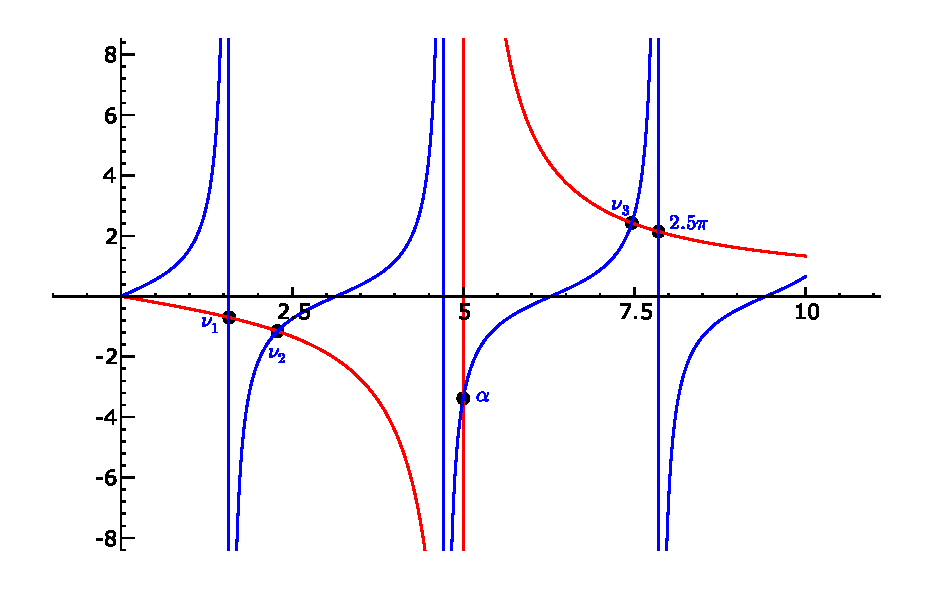
\includegraphics[width=\textwidth]{$HOME/book/fourier/img/2May2008img1.eps}
\caption[Eigenvalue Relations for Heat Equation]{A Plot of
  the Eigenvalue relations for the Heat Equation from Eq
  \eqref{eqn:2May2008:eigenvalueRelationship} setting
  $\alpha=5$ and $L=1$. The blue line is $\tan(\nu L)$, the
  red line is $2\alpha\nu/(\nu^2-\alpha^2)$. Note that the
  points labeled $\alpha$ and $2.5\pi$ are not eigenvalues
  but singular points of $2\alpha\nu/(\nu^2-\alpha^2)$ and
  $\tan(\nu L)$ respectively that coincidentally overlap in
  the graph program.}\label{fig:2May2008:eigenPlot}
\end{figure}

We were looking at the Sturm-Liouville problem which came
from the heat equation
\begin{equation}
X''(x)+\nu^{2}X(x) = 0
\end{equation}
with the boundary conditions
\begin{subequations}
\begin{align}
X'(0) &= \alpha X(0)\\
X'(L) &= -\alpha X(L)
\end{align}
\end{subequations}
With eigenfunctions $\{\nu\cos(\nu x) + \alpha\sin(\nu x)\}$
where the eigenvalues $\nu^2$ are determined by
\begin{equation}\label{eqn:2May2008:eigenvalueRelationship}
\tan(\nu L) = \frac{2\alpha\nu}{\nu^2-\alpha^2}
\end{equation}
But this isn't the most convenient way to determine the
eigenvalues, as it's not really convenient to do
analytically. The plot of the left hand side in blue and the
right hand side in red is given in figure
\eqref{fig:2May2008:eigenPlot}. We find that
$0<\nu_1<\nu_2<\cdots$. We can normalize the eigenfunctions
$\phi_{\nu}(x)$ to find
\begin{subequations}
\begin{align}
\|\phi_{\nu}\|^{2} &= \int^{L}_{0} (\nu\cos(\nu x)+\alpha\sin(\nu x))^2dx\\
&=\int^{L}_{0} \nu^{2}\cos^{2}(\nu x) + 2\alpha\nu\sin(\nu x)\cos(\nu x) + \alpha^{2}\sin^{2}(\nu x)dx
\end{align}
\end{subequations}
Remember from basic trigonometry
\begin{align*}
\cos^{2}\theta &= \frac{1}{2}(1 + \cos(2\theta))\\
\sin^{2}\theta &= \frac{1}{2}(1 - \cos(2\theta))
\end{align*}
so plugging this in we find
\begin{subequations}
\begin{align}
\|\phi_{\nu}(x)\|^{2} &=
\frac{\nu^2}{2}\int^{L}_{0}(1+\cos(2\nu x))dx +2\alpha\int^{L}_{0}\sin(\nu x)d\left(\sin(\nu x)\right) +\frac{\alpha^2}{2}\int^{L}_{0}(1-\cos(\nu x))dx\\
&=\left(\frac{\nu^2+\alpha^2}{2}\right)L+\alpha\sin^{2}(\nu L)+\int^{L}_{0}\frac{\nu}{2}\cos(2\nu x)-\frac{\alpha^2}{2}\cos(2\nu x)dx\\
&=\left(\frac{\nu^2+\alpha^2}{2}\right)L+\alpha\sin^{2}(\nu L)+\left(\frac{\nu^2-\alpha^2}{4\nu}\right)\sin(2\nu L)
\end{align}
\end{subequations}
We can now take advantage of our eigenrelations
\begin{equation}
\tan(\nu L) = \frac{2\alpha\nu}{\nu^2 - \alpha^2}
\end{equation}
to reduce our calculation of the norm of $\phi_{\nu}(x)$ to
be
\begin{equation}
\frac{1}{2}\left(\frac{\nu^2-\alpha^2}{2\nu}\right) =
\frac{1}{2}\frac{1}{\tan(\nu L)} = \frac{1}{2}\frac{\cos(\nu
  L)}{\sin(\nu L)}
\end{equation}
thus
\begin{subequations}
\begin{align}
\frac{\nu^2-\alpha^2}{2(2\nu)}\sin(\nu L) &=
\frac{1}{2}\cot(\nu L)2\sin(\nu L)\cos(\nu L)\\
&=\alpha\cos^{2}(\nu L)
\end{align}
\end{subequations}
So $\|\phi_{\nu}(x)\|^2 = [(1+L/2)\alpha^2 +
  \nu^2L/2]^{1/2}$, and the orthonormal basis formed for
$L^{2}(0,L)$ satisfies the problem 
\begin{equation}
\partial_{t}u(x,t) = k\partial_{x}^{2}u(x,t)
\end{equation}
where
\begin{equation}
u_{n}(x,t) = c_{n} e^{-\nu^{2}_{n}kt}\phi_{n}(x)
\end{equation}
We need to now find what all the $c_{n}$'s are. (Yes, our
work never ends; we're like Pinkerton's, we never rest.)

To do so, we let
\begin{subequations}
\begin{align}
u(x,t) &= \sum^{\infty}_{n=1}u_{n}(x,t) = \sum^{\infty}_{n=1}c_{n}e^{-\nu^{2}_{n}kt}\phi_{n}(x)\\
u(x,0)&=f(x)=\sum^{\infty}_{n=1}\<f,\phi_n\>\phi_n\\
&=\sum^{\infty}_{n=1}u_{n}(x,0)=\sum^{\infty}_{n=1}c_{n}\phi_{n}
\end{align}
\end{subequations}
Take the difference, we find
\begin{equation}
\sum^{\infty}_{n=1}(c_{n}-\<f,\phi_n\>)\phi_n=0
\end{equation}
because $\phi_n$ is a basis and this linear combination is
zero, we conclude that
\begin{equation}
c_{n} = \<f,\phi_n\>.
\end{equation}

\marginpar{Change boundary conditions}Lets change the
boundary conditions a bit to be
\begin{equation}
X''(x) + \nu^{2}X(x)=0,\qquad X(0)=X(L)=0
\end{equation}
This corresponds to the heat equation
\begin{equation}
\partial_{t}u(x,t) = k\partial^{2}_{x}u(x,t),\qquad
u(0,t)=u(L,t)=0
\end{equation}
The general solution of $X''(x)+\nu^2 X(x)=0$ is
\begin{equation}
X(x)=c_1\cos(\nu x)+c_2\sin(\nu x)
\end{equation}
Plug in the first boundary condition
\begin{equation}
X(0)=c_1=0\Rightarrow c_1=0
\end{equation}
Thus
\begin{equation}
X(x)=c_2\sin(\nu x)
\end{equation}
which is normalized to be the normalized eigenfunction
\begin{equation}
X(x)=\sin(\nu x).
\end{equation}
The eigenvalues are found by simpy plugging in the second
boundary condition
\begin{equation}
X(L)=0\Rightarrow \sin(\nu L)=0\Rightarrow \nu=n\pi/L
\end{equation}
The eigenvalues are thus
\begin{equation}
\nu_{n} = \frac{n}{L}\pi
\end{equation}
So the eigenfunctions form the set
$\{\sin(n\pi/L)\}^{\infty}_{1}$ which is the basis for
$L^{2}(0,L)$. We choose $n\in\mathbb{N}$ because $X(x)$ is
an odd function $X(-x)=-X(x)$. 

\begin{ex}
Consider an external source added to the heat equation
\begin{equation}
\partial_{t}u(x,t) = k\partial^{2}_{x}u(x,t) +
\underbracket{F(x,t)}_{\text{external source}}
\end{equation}
with the boundary conditions $u(0,t)=u(L,t)=0$ and
$u(x,0)=0$. For each $t$, the source $F(x,\cdot)$ is just a
function of $x$ and we know $F(x,\cdot)\in L^{2}(0,L)$. If
this is the case, we can expand $F$ in terms of the
eigenbasis we just obtained. So \emph{for each $t$} we
expand
\begin{equation}
F(x,t) =
\sum^{\infty}_{n=1}\beta_{n}(t)\sin\left(\frac{nx}{L}\pi\right)
\end{equation}
If we know the form of $F$, we can compute the $\beta_n$
coefficients directly.

We want to find $u(x,t)$, so we assume that $u(\cdot,t)\in
C^{1}(0,\infty)$ and $u(x,\cdot)\in C^{2}(0,L)$. We can
expand
\begin{equation}
u(x,t) = \sum^{\infty}_{n=1}\underbracket[0.5pt]{b_{n}(t)}_{\text{unknown}}\sin\left(\frac{nx}{L}\pi\right)
\end{equation}
where $b_{n}(t)$ is unknown. We need to find the
coefficients $b_{n}(t)$ then we've found $u(x,t)$. 

We can see that the boundary conditions are satisfied since
\begin{subequations}
\begin{align}
u(0,t) &= \sum^{\infty}_{n=1}b_{n}(t)(0) = 0\\
u(L,t) &= \sum^{\infty}_{n=1}b_{n}(t)(0) = 0
\end{align}
\end{subequations}
We also want the expansion to satisfy the initial condition
\begin{equation}
u(x,0)=0\Rightarrow b_{n}(0)=0\quad \forall n\in\mathbb{Z}
\end{equation}
We have one fact about $b_{n}(t)$.

We can plug our series into our differential equation to
find
\begin{subequations}
\begin{align}
\partial_{t}u(x,t) &= k\partial^{2}_{x}u(x,t)+F(x,t)\\
\sum^{\infty}_{n=1}
b_{n}'(t)\sin\left(\frac{nx}{L}\pi\right) &= k
\sum^{\infty}_{n=1}b_{n}(t)\left(\frac{-n^2\pi^2}{L^2}\right)\sin\left(\frac{nx}{L}\pi\right)+ \sum^{\infty}_{n=1}\beta_{n}(t)\sin\left(\frac{nx}{L}\pi\right)\\
\sum^{\infty}_{n=1}\left(b_{n}'(t) + \frac{n^2\pi^2}{L^2}kb_{n}(t)\right)\sin\left(\frac{nx}{L}\pi\right)
&= \sum^{\infty}_{n=1}\beta_{n}\sin\left(\frac{nx}{L}\pi\right)
\end{align}
\end{subequations}
Now we are kind of happy, but it would be great if we could
just associate the terms together? Well, we can, because the
$\sin(\cdots)$ functions form an orthonormal basis, so we
can then write
\begin{subequations}
\begin{align}
\sum^{\infty}_{n=1}\left(b_{n}'(t) + \frac{n^2\pi^2}{L^2}kb_{n}(t) - \beta_{n}(t)\right)\sin\left(\frac{nx}{L}\pi\right)&=0\\
\Rightarrow b_{n}'(t) + \frac{n^2\pi^2}{L^2}kb_{n}(t) -
\beta_{n}(t) &=0
\end{align}
\end{subequations}
Thus we have
\begin{equation}
b_{n}'(t) + \frac{n^2\pi^2}{L^2}kb_{n}(t) = \beta_{n}(t).
\end{equation}
Let $\lambda_{n} = kn^2\pi^2/L^2$, then we can solve
\begin{equation}
b_{n}'(t) + \lambda_{n}b_{n}(t) = \beta_{n}(t)
\end{equation}
via the method of integrating factor.\index{Method of Integrating Factor} We have the
integrating factor be
\begin{equation}
\exp(\int\lambda_ndt)=\exp(\lambda_nt)
\end{equation}
so we multiply both sides by this quantity to find
\begin{equation}
e^{\lambda_nt}b_{n}'(t) + \lambda_{n}e^{\lambda_nt}b_{n}(t)
= \beta_{n}(t)e^{\lambda_nt}.
\end{equation}
We see that we can simplify this to be
\begin{equation}
\frac{d}{dt}(e^{\lambda_nt}b_{n}(t)) =
\beta_{n}(t)e^{\lambda_nt}
\end{equation}
and we can intgrate both sides with respect to $t$ to find
\begin{subequations}
\begin{align}
\int^{t}_{0}\frac{d}{ds}(e^{\lambda_ns}b_{n}(s))ds &= \int^{t}_{0}e^{\lambda_ns}\beta_{n}(s)ds\\
e^{\lambda_ns}b_{n}(s)|^{t}_{0}&=\int^{t}_{0}e^{\lambda_ns}\beta_{n}(s)ds\\
e^{\lambda_nt}b_{n}(t)&=\int^{t}_{0}e^{\lambda_ns}\beta_{n}(s)ds\\
\Rightarrow b_{n}(t)&=e^{-\lambda_nt}\int^{t}_{0}e^{\lambda_ns}\beta_{n}(s)ds
\end{align}
\end{subequations}
SO we have just found the solution for $u(x,t)$ given some
$F(x,t)$ external source.
\end{ex}

Observe that we can do the same trick with the wave equation
\begin{equation}
\partial_{t}^{2}u(x,t) = c^{2}\partial_{x}^{2}u(x,t)
\end{equation}
with boundary conditions
\begin{equation}
u(0,t)=u(L,t)=0.
\end{equation}
We use the same Sturm-Liouville trick. We need more initial
conditions however
\begin{equation}
u(x,0)=f(x)\text{ and }\partial_{t}u(x,0)=g(x)
\end{equation}
We can expand both $f$ and $g$ in terms of the basis. When
we plug in
\begin{equation}
u(x,t) = \sum_{n}b_{n}(t)\phi_{n}(x)
\end{equation}
we find
\begin{equation}
b_{n}''(t) + \frac{c^2n^2\pi^2}{L^2}b_{n}(t) = 0
\end{equation}
So the general solution is
\begin{equation}
b_{n}(t) = c_{1}\cos\left(\frac{cn\pi}{L}t\right)+c_{2}\sin\left(\frac{cn\pi}{L}t\right)
\end{equation}
and we have just found the general solution in the form of a
series. 

%%%%
%%    Fourier Transform
%%%%
\part{Fourier Transforms}
\section{A Review of $L^{2}$ and an Introduction to the Fourier Transform}
%%
%% 5May2008.tex
%% 
%% Made by Alex Nelson
%% Login   <alex@tomato>
%% 
%% Started on  Sun Dec 21 19:01:05 2008 Alex Nelson
%% Last update Sun Dec 21 19:01:05 2008 Alex Nelson
%%
%% We will review the function space $L^{2}$ and $L^{1}$,
%% and we will introduce the Fourier transform

Note that for short hand usage we will write
$L^{2}=L^{2}(-\infty,\infty)$. More generally, we have
\begin{equation}
L^{p} = \{f\text{ defined on }\mathbb{R}:
\int^{\infty}_{-\infty}|f(x)|^pdx\}
\end{equation}
where $p\in\mathbb{N}$. In a very special case, when $p=2$,
we have a Hilbert space with an inner product defined by
\begin{equation}
\<f,g\> = \int^{\infty}_{-\infty}f(x)\overline{g(x)}dx
\end{equation}
and an induced norm
\begin{equation}
\|f\| = \sqrt{\<f,f\>}
\end{equation}
All of the fundamental properties of the inner product and
the norm still hold for arbitrary end points, so they still
hold here.

The Cauchy-Schwarz inequality still holds
\begin{equation}
|\<f,g\>|\leq\|f\|\|g\|
\end{equation}
or equivalently
\begin{equation}
|\int f(x)\overline{g(x)}dx|\leq\left(\int|f(x)|^2dx\right)^{1/2}\left(\int|g(x)|^2dx\right)^{1/2}
\end{equation}
This is not as useful as
\begin{equation}
\<|f|,|g|\>=\int|f(x)g(x)|dx\leq\|f\|\|g\|
\end{equation}
which some (e.g~\cite{textbook}) refer to as the Cauchy-Schwarz.

Now, if we examine $L^{1}$,\index{$L^{1}$} it doesn't really have an inner
product, but it has a norm defined on it
\begin{equation}
\|f\|_{1} = \int|f(x)|dx.
\end{equation}

\begin{rmk}
Observe that $L^{2}(a,b)\subset L^{1}(a,b)$ for intervals,
but this is not true for $L^{2}$ and $L^{1}$. There are
$f\in L^2$ but $f\notin L^{1}$, and similarly there are
$g\in L^{1}$ but $g\notin L^{2}$.
\end{rmk}

\begin{ex}
Let
\begin{equation}
f(x) = \begin{cases}x^{-2/3}&\text{when }x>1\\
0&\text{otherwise}\end{cases}
\end{equation}
Now
\begin{subequations}
\begin{align}
\int^{\infty}_{1}|f(x)|dx &= \int^{\infty}_{1}x^{-2/3}dx\\
&= \lim_{b\to\infty}3x^{1/3}|^{b}_{1}\\
&= 3(\lim_{b\to\infty}b^{1/3}-1)=\infty
\end{align}
\end{subequations}
which means that $f\notin L^{1}$. But
\begin{subequations}
\begin{align}
\int^{\infty}_{1}|f(x)|^{2}dx &=
\int^{\infty}_{1}x^{-4/3}dx\\
&= \lim_{b\to\infty}-3x^{-1/3}|^{b}_{1}\\
&= -3(\lim_{b\to\infty}b^{-1/3}-1)\\
&= -3(-1) = 3
\end{align}
\end{subequations}
Thus $f\in L^2$. So $L^1$ functions go to zero but not as
fast as $L^2$ functions.
\end{ex}

Similarly we may show that
\begin{equation}
g(x) = \begin{cases} x^{-2/3} &\text{if }0< x<1\\
0 &\text{otherwise}\end{cases}
\end{equation}
Then we may show that $g\in L^1$ but $g\notin L^2$.

We will now give a list of useful facts without proofs.

\begin{enumerate}
\item If $f\in L^1$ and $|f(x)|\leq M$ for all
  $x\in\mathbb{R}$, then $f\in L^2$. So
\begin{equation}
\int |f(x)|^2dx\leq M\int|f(x)|dx<\infty
\end{equation}
thus $f\in L^2$. In other words, $L^{1}\cap L^{2}$ (the set
of functions in both $L^1$ and $L^2$) contains bounded
functions in both spaces.
\item If $f\in L^{2}$, and $f(x)=0$ for $x$ outside the
  interval $[a,b]$, then $f\in L^{1}$. Consider
\begin{equation}
\int|f(x)|dx = \int^{b}_{a}|f(x)|dx =
\int^{b}_{a}1\cdot|f(x)|dx
\end{equation}
then by the Cauchy-Schwarz inequality
\begin{subequations}
\begin{align}
\int^{b}_{a}1\cdot|f(x)|dx&\leq\left(\int^{b}_{a}|f(x)|^2dx\right)\left(\int^{b}_{a}1^{2}dx\right)^{1/2}\\
&\leq\sqrt{b-a}\|f(x)\|^{1/2}_{2}<\infty
\end{align}
\end{subequations}
\end{enumerate}

\begin{defn}\index{Fourier Transform}
Let $f$ be a function defined on the whole real line. Then
the \textbf{Fourier transform} is
\begin{subequations}
\begin{align}
\widehat{f}(\xi) &= \int^{\infty}_{\infty}f(x)e^{-ix\xi}dx\\
&=\<f,e^{i\xi x}\>
\end{align}
\end{subequations}
for all $\xi\in\mathbb{R}$. This is the continuous analog
for the Fourier series coefficients.
\end{defn}

The inversion formula is, if $f\in L^2$, 
\begin{equation}
f(x) = \int \widehat{f}(\xi)e^{ix\xi}d\xi
\end{equation}
for $x\in\mathbb{R}$.

\subsection{Derivation of Fourier Transform}
On $L^{2}(-\pi,\pi)$, we have the orthogonal basis
$\{\exp(inx)\}^{\infty}_{-\infty}$. If we have $f\in
L^{2}(-\pi,\pi)$, we may write it in the basis
\begin{equation}
f(x) = \sum c_{n}e^{inx}
\end{equation}
where
\begin{equation}
c_{n} = \frac{1}{2\pi}\int^{\pi}_{-\pi}f(x)e^{-inx}dx
\end{equation}
If $f$ is $2\pi$-periodic then the expansion is defined
almost everwhere (at least it's defined on the interval
$[-\pi,\pi]$).

We may scale this to the interval $f\in L^{2}(-\ell,\ell)$
where $\ell>0$, then the basis becomes
\begin{equation}
\exp(inx)\to\exp\left(\frac{in\pi}{\ell}\right).
\end{equation}
The Fourier expansion then becomes
\begin{equation}
f(x) = \sum
\widetilde{c}_{n}e^{ix(n\pi/\ell)},\quad\text{where
}\widetilde{c}_n=\frac{1}{2\ell}\int^{\ell}_{-\ell}f(y)e^{-iny\pi/\ell}dy
\end{equation}
For $f$ defined on $\mathbb{R}$, we want to expand $f$ as a
superposition of $\exp(i\xi x)$...\textbf{HOW TO DO IT?!?}

For $[-\ell,\ell]$ when $\ell>0$. The Fourier expansion on
$[-\ell,\ell]$ and take the limit as $\ell\to\infty$:
\begin{equation}
f(x) = \sum^{\infty}_{-\infty}\frac{c_n}{2\ell}e^{in\pi
  x/\ell}
\end{equation}
where
\begin{equation}
c_n = \<f,e^{inx\pi/\ell}\> =
\int^{\ell}_{-\ell}f(x)e^{-inx\pi/\ell}dx
\end{equation}
We'll now turn this into a Riemann sum\index{Fourier Transform!Derived Using Riemann Sums}, let
\begin{equation}
\Delta\xi = \pi/\ell
\end{equation}
then subdividing the interval from $-\pi$ to $\pi$ into
\marginpar{Note interpretation of $\xi_n$ as boundaries of subintervals}$2\ell$ intervals. Let
\begin{equation}
\xi_n = n\Delta \xi = \frac{n\pi}{\ell} = \text{ endpoints of subintervals of }[-\pi,\pi]\index{$\xi_n$!As Dual To $x$}
\end{equation}
Then
\begin{subequations}
\begin{align}
f(x) &= \sum\frac{c_n}{2\ell}e^{in\pi x/\ell}\\
&=\sum c_n\frac{1}{2\ell}\cdot1\cdot e^{in\pi x/\ell}\\
&= \sum c_n\left(\frac{1}{2\ell}\right)\left(\frac{\Delta \xi}{\pi/\ell}\right)e^{i\xi_nx}\\
&= \sum c_n\left(\frac{1}{2\ell}\frac{\Delta \xi}{\pi/\ell}\right)e^{i\xi_nx}\\
&= \sum \frac{c_n}{2\pi}e^{i\xi_nx}\Delta \xi
\end{align}
\end{subequations}
where 
\begin{equation}
c_n = \int^{\ell}_{-\ell}f(y)\exp(-i\xi_{n}y)dy
\end{equation}
which when we take $\ell\to\infty$ is approximately
\begin{equation}
c_n\approx\int^{\infty}_{-\infty}f(y)e^{-i\xi_{n}y}dy
\end{equation}
provided $f$ vanishes rapidly as $y\to\pm\infty$. But this
is the definition of $\widehat{f}(\xi_n)$. We then make this
change to find $\Delta \xi\to d\xi$:
\begin{equation}
f(x)\approx \int^{\infty}_{-\infty}\frac{\widehat{f}(\xi_n)}{2\pi}e^{i\xi_nx}d\xi_n.
\end{equation}
Thus we finish our derivation of the Fourier transform.

\section{Convolution}
%%
%% 9May2008.tex
%% 
%% Made by Alex Nelson
%% Login   <alex@tomato>
%% 
%% Started on  Sun Dec 21 20:20:11 2008 Alex Nelson
%% Last update Sun Dec 21 20:20:11 2008 Alex Nelson
%%
\begin{defn}\index{Convolution}
The \textbf{convolution} of two functions is a function
defined by
\begin{equation}
(f*g)(x) = \int_{\mathbb{R}}f(x-y)g(y)dy
\end{equation}
provided that both integrals converge.
\end{defn}

\begin{ex}
Let $f(x)=x$, $g(x)=x^2$, $h(x)=\exp(-x^2)$, then
\begin{equation}
(f*g)(x) = \int^{\infty}_{-\infty}(x-y)y^2dy
\end{equation}
does not exist for arbitrary $x$. Thus the convolution is
not well defined. However,
\begin{equation}
(f*h)(x) = \int^{\infty}_{-\infty}(x-y)e^{-y^2}dy =
  \sqrt{\pi}x
\end{equation}
for all $x\in\mathbb{R}$.
\end{ex}
\begin{proof}{(Proof of outrageous claim)}
Compute
\begin{equation}
\int^{\infty}_{-\infty}e^{-y^2}dy = \sqrt{\pi}.
\end{equation}
We can take it on faith (which I'll do out of laziness), or
we can bust open a can of complex analytical whoop ass on
the problem and use residues. We have
\begin{equation}
(f*h)(x)=x\int_{\mathbb{R}}e^{-y^{2}}dy - \int_{\mathbb{R}}ye^{-y^2}dy
\end{equation}
we see that $y\exp(-y^2)$ is odd, so its integral from
$-\infty$ to $+\infty$ vanishes. We are left with
\begin{equation}
(f*h)(x)=x\int_{\mathbb{R}}e^{-y^2}dy
\end{equation}
and this is necessarily
\begin{equation}
(f*h)(x) = x\sqrt{\pi}
\end{equation}
which concludes our proof.
\end{proof}

Note
\begin{equation}
|(f*g)(x)|\leq\int|f(x-y)g(y)|dy
\end{equation}
so if the integral converges absolutely, then the
convolution exists. \marginpar{convolution gauranteed when...}Some cases when the convolution is guarenteed:
\begin{enumerate}
\item $f\in L^{1}(\mathbb{R})$, $|g(x)|\leq M$ for all
  $x\in\mathbb{R}$, the integral converges absolutely
\item $g\in L^{1}(\mathbb{R})$, $|f(x)|\leq M$ for all
  $x\in\mathbb{R}$, then the convlution exists
\begin{equation}
\int|f(x-y)g(y)|dy\leq M\int|f(x-y)|dy<+\infty
\end{equation}
\item $f,g\in L^{2}(\mathbb{R})$, we have
\begin{equation}
\int|f(x-y)g(y)|dy\leq\left(\int|f(x-y)|^2dy\right)^{1/2}\left(\int|g(y)|^2dy\right)^{1/2}<+\infty
\end{equation}
where we justify making it less than infinity by the
properties of $L^2$.
\end{enumerate}
There are many more times whene convolution is gauranteed.

But \textbf{WTF does the convolution mean anyways?}

Recall that the average of a function on $[a,b]$ is
\begin{equation}
avg(f) = \frac{1}{b-a}\int^{b}_{a}f(x)dx
\end{equation}
We can generalize this to be a weighted average on $[a,b]$:
\begin{equation}
wt(f) = \frac{\int^{b}_{a}f(x)\omega(x)dx}{\int^{b}_{a}\omega(x)dx}
\end{equation}
For our typical average, we usually just set
$\omega(x)=1$. So for
\begin{equation}
(f*g)(x)
  = \begin{pmatrix}$weighted$\ $average$\ $of$\ g\ $around$\\
$the$\ $point$\ x $ with$\ $the$\ $weight$\\ 
$determined$\ $by$\ $the$\ $function$\ f,\\ 
$provided$\ f $ is$\ $normalized$\\ 
\int f(x)dx=1\end{pmatrix}
\end{equation}

Alternatively, we can observe
\begin{equation}
(f*g)(x) = \int f(x-y)g(y)dy
\end{equation}
so by plugging in the Riemann sum for the integral, we have
\begin{equation}
\int f(x-y)g(y)dy \approx \sum f(x-y_j)g(y_j)\Delta y_j.
\end{equation}
The function $f(x-y_j)$ is just the function $f$ translated
along the $x$ axis by the amount $y_j$, so the sum on the
right is a linear combination of translates of $f$ with
coefficients $g(y_j)\Delta y_j$. 

\begin{ex}
Let
\begin{equation}
f = \begin{cases}1&\text{if }|x|\leq a\\
0&\text{otherwise}\end{cases}
\end{equation}
We normalize this to be
\begin{equation}
f = \begin{cases}\frac{1}{2a}&\text{if }|x|\leq a\\
0&\text{otherwise}\end{cases}
\end{equation}
So $\int^{\infty}_{-\infty}f(x)dx = 1$. Then for any $g$
such that the convolution with $f$ exists
\begin{subequations}
\begin{align}
(f*x)(x) &= \int f(x-y)g(y)dy\\
&= \int_{|x-y|\leq a} \frac{g(y)}{2a}dy\\
&= \int_{x-a} \frac{g(y)}{2a}dy\\
&=\text{average of $g$ on interval $[x-a,x+a]$}
\end{align}
\end{subequations}
\end{ex}


\begin{figure}[h!]
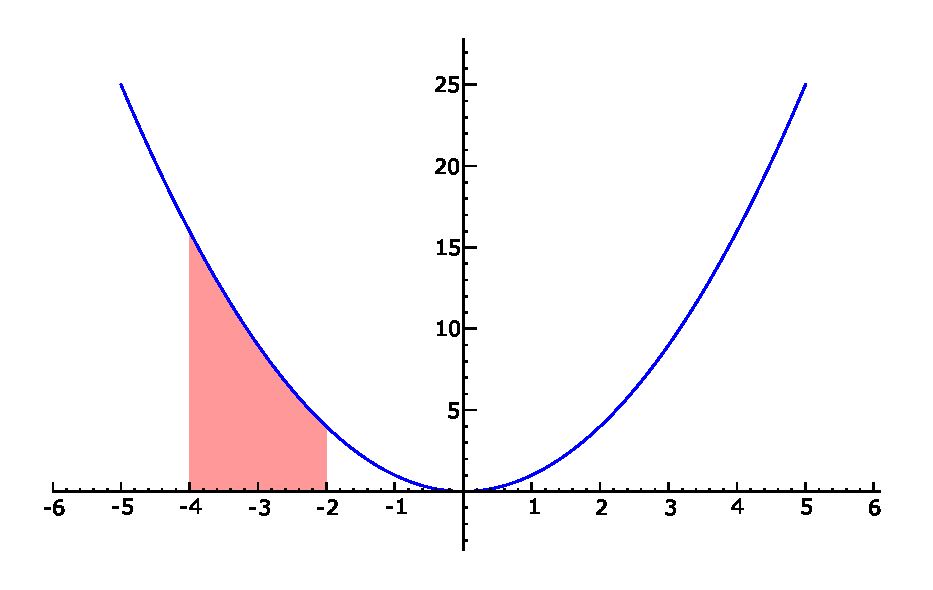
\includegraphics[width=0.45\textwidth]{$HOME/book/fourier/img/9May2008img1.eps}
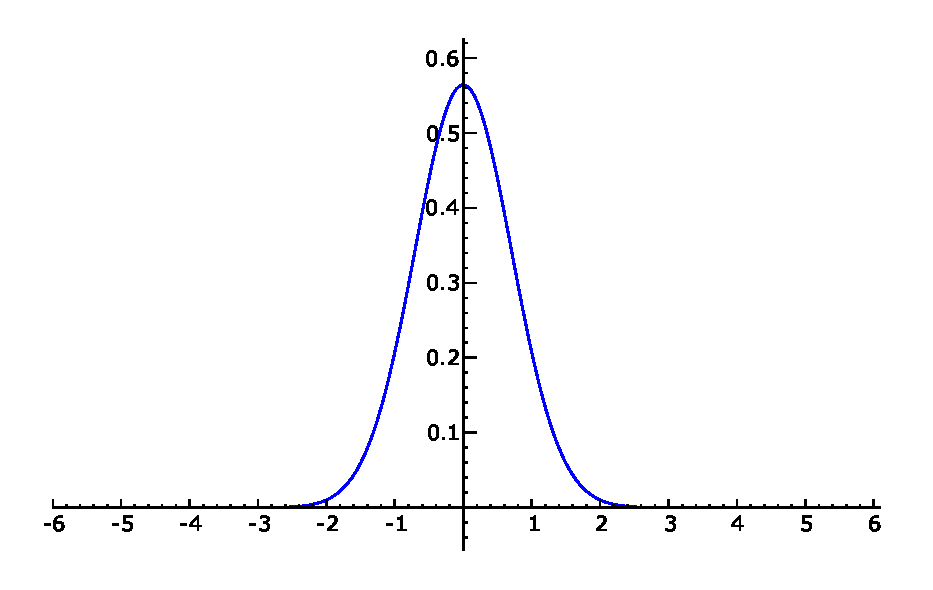
\includegraphics[width=0.45\textwidth]{$HOME/book/fourier/img/9May2008img2.eps}
\caption{On the left, convolution with $x^2$; on the right, the Gaussian Kernel.}\label{img:9May2008:img1}\label{img:9May2008:img2}
\end{figure}

%% \begin{figure}
%% \subfigure[Convolution with $x^2$]{\label{img:9May2008:img1}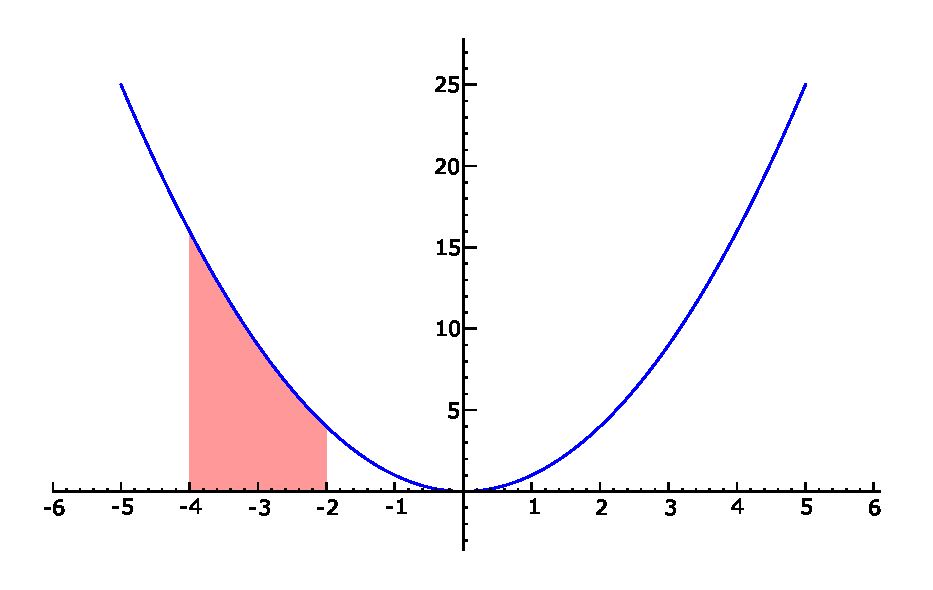
\includegraphics[width=0.45\textwidth]{$HOME/book/fourier/img/9May2008img1.eps}}
%% \subfigure[Gaussian Kernel]{\label{img:9May2008:img2}w
%% \end{figure}

\begin{ex}
Let $g(x)=x^2$, consider the convolution
$(f*g)(x)$. Convolution is just sliding $f$ along the $x$ 
axis. You can see the integral as the red shaded region of
figure \eqref{img:9May2008:img1}.
\end{ex}

\begin{ex}
Let $f(x)=\exp(-x^2)$ and $g(x)=x^2$. Then we first
normalize $f(x)$ by introducing
$\widetilde{f}(x)=f(x)/\sqrt{\pi}$ so we see
\begin{equation}
\int\widetilde{f}(x)dx = 1.
\end{equation}
This is a special function called the Gaussian
Kernel\index{Gaussian Kernel}\marginpar{Gaussian Kernel}
\begin{equation}
  \addtolength{\fboxsep}{5pt}
   \boxed{
   \begin{gathered}
     \widetilde{f}(x) = \frac{e^{-x^2}}{\sqrt{\pi}}
   \end{gathered}
   }
\end{equation}
For $|x|\geq 4$, $\widetilde{f}(x)\leq 6.4\times
10^{-8}$. The values of $\widetilde{f}(x)$ that really
matter are between $[x-4,x+4]$. One can see this reflected
in the plot of the Gaussian in figure \eqref{img:9May2008:img2}.

Suppose we shrink this down to
$[x-\varepsilon,x+\varepsilon]$ for small $\varepsilon$ by
scaling or ``dilating'' $f$. We do this, given $\int
f(x)dx=1$, we define\marginpar{Scaling or Dilations} the 
\textbf{scaling}\index{Scaling} or \textbf{dilation}\index{Dilation}
of $f$ is given as
\begin{equation}
f_{\varepsilon}(x) = \frac{1}{\varepsilon}f\left(\frac{x}{\varepsilon}\right)
\end{equation}
For $f(x)=\exp(-x^2)/\sqrt{\pi}$, we have
\begin{equation}
f_{\varepsilon}(x) = \frac{1}{\varepsilon\sqrt{\pi}}\exp(-(x/\varepsilon)^2).
\end{equation}
As $\varepsilon$ gets smaller, the peak gets higher, so
$f_{\varepsilon}(x)\leq(6.4\times10^{-8})/\varepsilon$ for
$|x|\geq4\varepsilon$. What then is
\begin{subequations}
\begin{align}
(f_{\varepsilon}*g)(x) &= \frac{1}{\varepsilon\sqrt{\pi}}\int\exp\left[-\left(\frac{x-y}{\varepsilon}\right)^{2}\right]g(y)dy\\
&\approx \frac{1}{\varepsilon\sqrt{\pi}}\int^{x+4\varepsilon}_{x-4\varepsilon}\exp\left[-\left(\frac{x-y}{\varepsilon}\right)^{2}\right]g(y)dy
\end{align}
\end{subequations}
\end{ex}

%%
%% 12May2008.tex
%% 
%% Made by Alex Nelson
%% Login   <alex@tomato>
%% 
%% Started on  Sun Dec 21 21:55:49 2008 Alex Nelson
%% Last update Sun Dec 21 21:55:49 2008 Alex Nelson
%%

\begin{thm}
Convolution has the same algebraic properties as
multiplication
\begin{enumerate}
\item $f*(\alpha g+\beta h) = \alpha(f*g)+\beta(f*h)$
\item $f*g=g*f$ to prove this, do a change of variables
\begin{align*}
(f*g)(x) &= \int f(x-y)g(y)dy,\quad\text{let }z=x-y\\
&=\int f(z)g(x-z)dz\\
&=(g*f)(x)
\end{align*}
\item $f*(g*h)=(f*g)*h$
\end{enumerate}
\end{thm}
\begin{thm}{(Convolution increases Smoothness)}
Suppose $f$ is differentiable, $f*g$ and $f'*g$ are well
defined (i.e. exist), then $f*g$ is differentiable and
\begin{equation}
(f*g)' = f'*g
\end{equation}
\end{thm}
\begin{proof}
Observe
\begin{equation}
(f*g)'(x) = \frac{d}{dx}\int f(x-y)g(y)dy
\end{equation}
The integral converges for all $x$ and $x$ is not the
variable of integration, so
\begin{align*}
\frac{d}{dx}\int f(x-y)g(y)dy &= \int\frac{d}{dx}\Big(f(x-y)g(y)\Big)dy\\
&=\int f'(x-y)g(y)dy\\
&=(f'*g)(x)
\end{align*}
which concludes our proof.
\end{proof}

\textbf{Implication:} $g$ may not have any derivatives, but
if $g\in C^{\infty}(\mathbb{R})$, then we may form a new
function $(f*g)$ which inherits all the smoothness of $g$,
i.e. $(f*g)\in C^{\infty}$.

\textbf{Three $C^\infty$ functions}
\begin{enumerate}
\item The Gaussian Kernel, which we have already seen,
\begin{equation}
G(x) = \frac{1}{\sqrt{\pi}}e^{-x^2}
\end{equation}
with the conditions that $\int G(x)dx=1$, it's even, and
$G(x)\in C^{\infty}(\mathbb{R})$. Additionally, it's bounded!
\item The standard Cauchy distribution is another good
  choice
\begin{equation}
H(x) = \frac{1}{\pi}\frac{1}{1+x^2}
\end{equation}
$\int H(x)dx=1$, $H(x)\in C^{\infty}(\mathbb{R})$, $H(x)$ is
even, it's bounded too.
\item The last is
\begin{equation}
K(x) = \begin{cases} \frac{1}{c}e^{-1/(1-x^2)} &\text{when }|x|<1\\
0&\text{otherwise}\end{cases}
\end{equation}
where $C=\int^{1}_{-1}\exp(-1/(1-x^2))dx$, $K(x)\in
C^{\infty}(\mathbb{R})$, the only time we worry is at
$x=\pm1$. But it's clear that $\exp(-1/(1-x^2))$ vanishes
for all derivatives of it. It's bounded, vanishes outside
the interval from $[-1,1]$.
\end{enumerate}

Suppose $g\in L^1$, $\int gdx=1$, dilates of $g$ are --- for
any $\varepsilon>0$ ---
\begin{equation}
g_{\varepsilon}(x) =
\frac{1}{\varepsilon}g\left(\frac{x}{\varepsilon}\right)
\end{equation}
If $g'(x)$ exists, then
\begin{equation}
g_{\varepsilon}'(x) =
\frac{1}{\varepsilon^2}g'\left(\frac{x}{\varepsilon}\right).
\end{equation}

For the next theorem, let $\int g(x)dx=1$, 
$$\alpha = \int^{0}_{-\infty}g(x)dx$$
and
$$\beta = \int^{\infty}_{0}g(x)dx$$
so $\alpha+\beta=1$. If $g$ is even, then
$$\alpha=\beta=\frac{1}{2}.$$
\begin{thm}\label{thm:12May2008:thmUsedInInverseFourierTransform}
Suppose $g\in L^1$, and $\int g(x)dx=1$. Suppose $f\in
PC(\mathbb{R})$, and aso suppose either $|f(x)|\leq M$ for
all $x\in\mathbb{R}$ or $g(x)=0$ for $x$ outside some finite
interval, so $f*g$ is well defined. Then
\begin{equation}
\lim_{\varepsilon\to0}(f*g)_{\varepsilon}(x) = \alpha
f(x^+)+\beta f(x^-)
\end{equation}
for all $x\in\mathbb{R}$. SO if $x$ is continuous at $x$
then
$\lim_{\varepsilon\to0}(f*g)_{\varepsilon}(x)=f(x)$. (This
means that $|(f*g)_{\varepsilon}(x)-\alpha f(x^+)-\beta
f(x^-)|<\delta$ for some $\delta>0$ when $\varepsilon$ is
small enough; i.e. it's pointwise convergence.)

\emph{Alternatively} (if additionally supposing that
$|g(x)|\leq M$ for all $x$, and $f\in L^2$), then
$(f*g)_{\varepsilon}\stackrel{(\varepsilon\to0)}{\longrightarrow}f$
in norm.
\end{thm}

\section{Examples and Basic Properties of Fourier Transform}
%%
%% 14May2008.tex
%% 
%% Made by Alex Nelson
%% Login   <alex@tomato>
%% 
%% Started on  Fri Dec 26 17:02:27 2008 Alex Nelson
%% Last update Fri Dec 26 17:02:27 2008 Alex Nelson
%%
%% Fourier transforms

Let us consider a few examples computing the Fourier
transform of a function. Remember the Fourier transform is
\begin{equation}
\widehat{f}(\xi) = \int f(x)e^{-i\xi x}dx.
\end{equation}

\begin{ex}
Let
\begin{equation}
\chi_a(x) = \begin{cases} 1 & \text{if }|x|<a\\
0 & \text{otherwise}\end{cases}
\end{equation}
be a characteristic function. Then
\begin{subequations}
\begin{align}
\widehat{\chi}_{a}(\xi) &= \int^{a}_{-a}\xi_{a}(x)e^{-i\xi
  x}dx\\
&= \int^{a}_{-a}e^{-i\xi x}dx\\
&= \frac{i}{\xi}(e^{ia\xi}-e^{-ia\xi})\\
&= -2\frac{\sin(a\xi)}{\xi}.
\end{align}
\end{subequations}
\end{ex}
\begin{ex}
Consider
\begin{equation}
\mathcal{F}\left[e^{-ax^{2}/2}\right] = \sqrt{\frac{2\pi}{a}}e^{-\xi^{2}/2a}
\end{equation}
where $\mathcal{F}[\cdot]$ is the fourier transform. We can
see that
\begin{subequations}
\begin{align}
\mathcal{F}\left[e^{-ax^{2}/2}\right] &= \int
e^{-ax^{2}/2-i\xi x}dx\\
&=\int e^{-y^2+(\xi^{2}/a)}\left(\frac{2}{\sqrt{a}}\right)dy \quad\text{where } y=x\sqrt{a/2}+i\xi/\sqrt{2a}\\
&=\sqrt{\frac{2}{a}}e^{-\xi^{2}/2a}\int e^{-y^2}dy\\
&=\sqrt{\frac{2\pi}{a}}e^{-\xi^{2}/2a}.
\end{align}
\end{subequations}
Since we know that 
\begin{equation}
\int e^{-x^2}dx = \sqrt{\pi}.
\end{equation}
\end{ex}

Now let us consider some of the basic properties of the
Fourier transform.
\begin{enumerate}
\item{(Shifting the Fourier Transform\index{Fourier Transform!Shift})} For $a\in\mathbb{R}$, 
\begin{align*}
\mathcal{F}\left[f(x-a)\right] &=
e^{-ia\xi}\mathcal{F}[f(x)]\\
&= e^{-a\xi}\widehat{f}(\xi)
\end{align*}
\item{(Dilation\index{Fourier Transform!Dilation})} For $\delta>0$, $f_{\delta}(x) = f(x/\delta)/\delta$,
  then $\mathcal{F}(f_{\delta}) =
  \widehat{f}(\delta\xi)$. If $\delta>1$, we're shrinking
  the width of $f$, but expanding the width of
  $\widehat{f}$. We also have
\begin{equation}
\mathcal{F}\left[f(\delta x)\right] =
\widehat{f}_{\delta}(\xi)
\end{equation}
\item\marginpar{Most important property of Fourier Transform!} If
$f$ is continuous, its first derivative $f'(x)\in
  PC(\mathbb{R})$ is piecewise continuous, and $f\in L^{1}$,
  then
\begin{equation}
\mathcal{F}\left[\frac{d}{dx}f(x)\right](\xi) = i\xi\widehat{f}(\xi).
\end{equation}
This should be familiar, recall that fo the Fourier series
we have $f$ has coefficients $c_n$ and $f'$ has coefficients
$inc_n$. On the other hand, if $xf(x)\in L^{1}$, then
\begin{equation}
\mathcal{F}\left[xf(x)\right](\xi) = i\frac{d}{d\xi}\widehat{f}(\xi).
\end{equation}
\item If both $f,g\in L^{1}$, then
\begin{equation}
\mathcal{F}[f*g](\xi) = \widehat{f}(\xi)\widehat{g}(\xi)
\end{equation}
\end{enumerate}
The last property is the most important as it lets us change
a given differential equation into an algebraic equation.
\begin{proof}
\begin{enumerate}
\item{(Shift)} We see that
\begin{align*}
\mathcal{F}[f(x-a)] &= \int f(x-a)e^{-ix\xi}dx \\
&= \int f(y)e^{-i\xi(y+a)}dy\quad\text{where }y=x-a\\
&= e^{-ia\xi}\int f(y)e^{-i\xi y}dy\\
&= e^{-a\xi}\widehat{f}(\xi).
\end{align*}
\item{(Dilation)} Again by direct computation we see that
\begin{align*}
\mathcal{F}[f_{\delta}](\xi) &= \int \frac{1}{\delta}f\left(\frac{x}{\delta}\right)e^{-ix\xi}dx\\
&=\int f(y)e^{-i\delta y\xi}dy,\quad\text{with }y=x/\delta\\
&=\int f(y)e^{-iy(\delta\xi)}dy\\
&=\mathcal{F}[f(x)](\delta\xi) = \widehat{f}(\delta\xi)
\end{align*}
\item{(Differentiation)} Observe, once more by direct
  computation
\begin{align*}
\mathcal{F}\left[\frac{d}{dx}f(x)\right] &= \int
f'(x)e^{-ix\xi}dx\\
&=f(x)e^{-ix\xi}|^{\infty}_{-\infty} - \int
f(x)\frac{d}{dx}e^{-i\xi x}dx 
\end{align*}
where we have just done integration by parts in the second
step. We see that since $f\in L^1$ that $f(x)\to 0$ as
$x\to\pm\infty$. So
\begin{align*}
f(x)e^{-ix\xi}|^{\infty}_{-\infty} - \int
f(x)\frac{d}{dx}e^{-i\xi x}dx  &= -\int
f(x)\frac{d}{dx}e^{-i\xi x}dx\\
&= \int f(x)i\xi e^{-ix\xi}dx\\
&= i\xi \int f(x)e^{-ix\xi}dx\\
&= i\xi \widehat{f}(\xi)
\end{align*}
Similarly, we see that 
\begin{equation}
xe^{-ix\xi} = i\frac{d}{d\xi}e^{-ix\xi}
\end{equation}
so
\begin{align*}
\mathcal{F}[xf(x)] &= \int xf(x)e^{-ix\xi}dx\\
&= \int \left(i\frac{d}{d\xi}e^{-i\xi x}\right)f(x)dx\\
&= i\frac{d}{d\xi}\int f(x)e^{-ix\xi}dx\\
&= i\frac{d}{d\xi}\widehat{f}(\xi)
\end{align*}
\item If 
\begin{align*}
\mathcal{F}[f*g](\xi) &= \int\left(\int f(x-y)g(y)dy\right)e^{-ix\xi}dx\\
&= \int\int f(x-y)g(y)e^{-ix\xi}dxdy
\end{align*}
Let $z=x-y$, then
\begin{align*}
\int\int f(x-y)g(y)e^{-ix\xi}dxdy&=\int\int f(z)e^{-i\xi(z+y)}dz g(y)dy\\
&=\int\left(\int f(z)e^{-i\xi(z+y)}dz\right)g(y)dy\\
&=\int\left(\int f(z)e^{-i\xi z}e^{-iy\xi}dz\right)g(y)dy\\
&=\int\left(\int f(z)e^{-iz\xi}dz\right)g(y)e^{-iy\xi}dy\\
&=\int\widehat{f}(\xi)e^{-iy\xi}g(y)dy\\
&=\widehat{f}(\xi)\int g(y)e^{-iy\xi}dy\\
&=\widehat{f}(\xi)\widehat{g}(\xi)
\end{align*}
which concludes our proof.
\end{enumerate}
\end{proof}

\begin{riemleb}
If $f\in L^{1}$, then $\mathcal{F}[f](\xi)\to0$ as $\xi\to\pm\infty$.
\end{riemleb}
\begin{sketch}
Intuitively we see
\begin{align*}
\widehat{f}(\xi) &= \int e^{-i\xi x}f(x)dx\\
&= \int e^{-iz}f(z)\frac{dz}{\xi}\\
|\widehat{f}(\xi)| &\leq
\int\left|f\left(\frac{z}{\xi}\right)\right|\frac{dz}{|\xi|}
= \frac{1}{|\xi|}\int\left|f\left(\frac{z}{\xi}\right)\right|dz\\
&\leq \frac{1}{|\xi|}k
\end{align*}
where $k$ is a constant, since $f\in L^{1}$. So
\begin{equation}
\lim_{\xi\to\pm\infty}f(\xi)\leq\lim_{\xi\to\pm\infty}\frac{1}{|\xi|}k
= 0.
\end{equation}
This concludes our sketch of the proof.
\end{sketch}
%%%%%%%%
%%%%%%%%
%%%% This is supposed to be part of 16 May 2008
%%%% 
%%%%%%%%
%%%%%%%%
What's the implication of the Riemann-Lebesgue lemma? Well,
in addition to the property (3) of the Fourier transform, it
implies the following:
\begin{quote}
If $f$ is smooth, $\widehat{f}$ decays quickly. If
$\widehat{f}$ decays fast, then $f$ is smooth.
\end{quote}
\begin{ex}
If $f\in C^{(k-1)}$, $f^{(k)}\in PC(\mathbb{R})$ and
$f^{(k)}\in L^{1}$, then we have
\begin{equation}
\mathcal{F}[f^{(k)}] = (i\xi)^{k}\widehat{f}(\xi).
\end{equation}
The Riemann-Lebesgue lemma says
$(i\xi)^{k}\widehat{f}(\xi)\to -$ as $|\xi|\to\infty$.
\end{ex}

\section{Inverse Fourier Transform, Fourier Transform on $L^2$}
%%
%% 16May2008.tex
%% 
%% Made by Alex Nelson
%% Login   <alex@tomato>
%% 
%% Started on  Fri Dec 26 18:15:38 2008 Alex Nelson
%% Last update Fri Dec 26 18:15:38 2008 Alex Nelson
%%
%% Fourier inversion formula, applications

\begin{lem}
If $f\in L^{1}$, then $\widehat{f}$ is continuous.
\end{lem}
\begin{proof}
Observe by direct computation
\begin{align*}
|\widehat{f}(\xi)-\widehat{f}(\eta)| &=
\left|\int\left(e^{-i\xi x}-e^{-i\eta
  x}\right)f(x)dx\right|\\
&\leq 2\int|f(x)|dx\quad\forall\eta,\xi\\
&\leq \int\left|e^{-i\xi x}-e^{-i\eta x}\right||f(x)|dx
\end{align*}
But as $\xi\to\eta$, $e^{-i\xi x}-e^{-i\eta x}\to 1-1=0$, so
the quantity
\begin{equation}
\int\left|e^{-i\xi x}-e^{-i\eta x}\right||f(x)|dx\to 0
\end{equation}
which concludes our proof.
\end{proof}
The Fourier transform so far has been shown to be one way,
mapping functions of $x$ to functions of $\xi$. Can we go
the other way? That is to say, is the Fourier transform
invertible\marginpar{Inverse Fourier Transform}?

\begin{invFourier}\index{Fourier Inversion Theorem}\index{Fourier Transform!Inverse}\index{Inverse Fourier Transform}
Suppose $f\in L^{1}$ and $f\in PC(\mathbb{R})$, then
\begin{equation}
\lim_{\varepsilon\to0}\frac{1}{2\pi}\int e^{i\xi x}e^{-\varepsilon^2\xi^2/2}\widehat{f}(\xi)d\xi=\frac{1}{2}\left[f(x^+)+f(x^-)\right]
\end{equation}
for all $x\in\mathbb{R}$. Moreover if both $f,\widehat{f}\in
L^{1}$, then $f$ is continuous, and
\begin{equation}
f(x) = \frac{1}{2\pi}\int e^{i\xi x}\widehat{f}(\xi)d\xi
\end{equation}
for all $x\in\mathbb{R}$.
\end{invFourier}
\begin{proof}
We have
\begin{equation}
\frac{1}{2\pi}\int e^{i\xi x}e^{-\varepsilon^2\xi^2/2}\widehat{f}(\xi)d\xi = \frac{1}{2\pi}\int e^{i\xi x}e^{-\varepsilon^{2}\xi^2/2}\int e^{-i\xi y}f(y)dyd\xi
\end{equation}
We can interchange the variables of integration, thus
\begin{align*}
\frac{1}{2\pi}\int e^{i\xi x}e^{-\varepsilon^{2}\xi^2/2}\int e^{-i\xi y}f(y)dyd\xi
&= \frac{1}{2\pi}\int\int e^{-i\xi(x-y)}e^{-\varepsilon^2\xi^2/2}f(y)d\xi dy\\
&= \frac{1}{2\pi}\int f(y)\left[\int e^{-i\xi(y-x)}e^{-\varepsilon^{2}\xi^2/2} \right]dy\\
&= \frac{1}{2\pi}\int f(y)\left[\sqrt{\frac{2\pi}{\varepsilon^2}}e^{-(y-x)^2/2\varepsilon^2}\right]dy\\
&= \frac{1}{\varepsilon\sqrt{2\pi}}\int f(y)e^{-(y-x)^{2}/2\varepsilon^2}dy\\
&=(f*\phi_{\varepsilon})(x)
\end{align*}
It turns out that $\phi(x) = \exp(-x^2/2)/\sqrt{2\pi}$ is
the Gaussian. This function is even, and integral is
evaluated to one. So it's $C^\infty$. By theorem \eqref{thm:12May2008:thmUsedInInverseFourierTransform},
$f*\phi_{\varepsilon}(x)\to\frac{1}{2}[f(x^-)+f(x^+)]$.

Suppose $f\in L^{1}$, then we need to show $f$ is
continuous. Since
\begin{equation}
|e^{i\xi x}e^{-\varepsilon^2\xi^2/2}\widehat{f}(\xi)|\leq|\widehat{f}(\xi)|
\end{equation}
for all $\xi$. We see that $|\exp(-\varepsilon^2\xi^2/2)|<1$
and $|\exp(i\xi x)|=1$. So
\begin{equation}
\int e^{i\xi
  x}e^{-\varepsilon^2\xi^2/2}\widehat{f}(\xi)d\xi\leq
\int|\widehat{f}(\xi)|d\xi = \|\widehat{f}\|_{L^1}
\end{equation}
for all $\varepsilon>0$. So
\begin{align*}
\mathcal{F}\{\widehat{f}\}(-x) &= \frac{1}{2\pi}\int e^{i\xi x}\widehat{f}(\xi)d\xi\\
&=\frac{1}{2\pi}\int e^{i\xi x}\left(\lim_{\varepsilon\to0}e^{-\varepsilon^2\xi^2/2}\right)\widehat{f}(\xi)d\xi\\
&=\lim_{\varepsilon\to0}\frac{1}{2\pi}\int e^{i\xi x}e^{-\varepsilon^2\xi^2/2}\widehat{f}(\xi)d\xi\\
&=\frac{1}{2}[f(x^+)+f(x^+)]\\
&= f(x)
\end{align*}
where we justify the last step since $f$ is continuous. So
$\mathcal{F}\{\widehat{f}\}(-x)$ is continuous since
$\widehat{f}\in L^1$, therefore $f$ is continuous so we're done.
\end{proof}

\begin{rmk}
If $f\in L^{1}$ and $f\in PC$, then $\widehat{f}$ may not be
in $L^1$. So we only have an approximation, which is the
first part of the theorem, then
\begin{equation*}
\underbracket[0.5pt]{e^{-\varepsilon^2\xi^2/2}\widehat{f}(\xi)}_{\text{approx
    of }\widehat{f}}=\underbracket[0.5pt]{\mathcal{F}\left\{f*\left(\frac{1}{\sqrt{2\pi}\varepsilon}e^{-(x/\varepsilon)^2/2}\right)\right\}}_{\text{approaches $f$ as $\varepsilon\to0$}}
\end{equation*}
\end{rmk}

\subsection{Consequences of the Inversion Theorem}

\begin{enumerate}
\item If $\widehat{f}=\widehat{g}$, then
  $\widehat{F}\{f-g\}=\widehat{f}-\widehat{g}=0$ which
  implies $f=g$. Thus the Fourier transform is
  unique\index{Fourier Transform!Uniqueness}. Further
  $\mathcal{F}^{-1}$ is well defined exactly by the
  inversion formula.
\item We have $\phi(x) = \exp(-x^2/2)/\sqrt{2\pi}$ in the
  inversion formula can be replaced by any (normalized)
  $g\in L^1$ with $\widehat{g}\in L^1$.
\item If $f\in L^1$, $\widehat{f}\in L^1$, then $f$ is
  continuous and $f\in L^2$. So
\begin{equation}
\int |f(x)|^2dx = \int|f(x)|\left|\int e^{i\xi x}\widehat{f}(\xi)d\xi\right|dx
\end{equation}
but
\begin{align*}
\left|\int e^{i\xi x}\widehat{f}(\xi)d\xi\right| &\leq
\int\left|e^{i\xi x}\widehat{f}(\xi)\right|d\xi\\
&\leq\int|\widehat{f}(\xi)|d\xi
\end{align*}
thus
\begin{align*}
\int|f(x)|^2dx &\leq \int|f(x)||\widehat{f}(\xi)|d\xi dx\\
&\leq \int|\widehat{f}(\xi)|d\xi\int|f(x)|dx.
\end{align*}
\end{enumerate}

\subsection{Fourier Transform on $L^2$}

Let $f\in L^2$, then $\widehat{f}(\xi)=\int\exp(-i\xi
x)f(x)dx$ converges in $L^2$ norm. This exists for almost
every $\xi$. Similarly
\begin{equation}
f(x) = \frac{1}{2\pi}\int e^{i\xi x}\widehat{f}(\xi)d\xi
\end{equation}
for almost every $x$.

\begin{plancherel}\index{Plancherel's Theorem}\index{Fourier Transform!In $L^2$}\index{Fourier Transform!Plancherel's Theorem}
The Fourier Transform is an operator
\begin{equation}
\mathcal{F}:L^2\to L^2
\end{equation}
and $\<\widehat{f},\widehat{g}\>=2\pi\<f,g\>$. If this is
the case, this implies 
\begin{equation}
\|\widehat{f}\|^{2} = 2\pi\|f\|^2.
\end{equation}
This is our Parseval identity in the continuous
case.\index{Parseval Equality!Fourier Transform}
\end{plancherel}
\begin{proof}
We see by direct computation
\begin{align*}
2\pi\<f,g\> &= 2\pi\int f(x)\overline{g(x)}dx\\
&=\frac{2\pi}{2\pi}\int
f(x)\overline{\int\widehat{g}(\xi)e^{i\xi x}d\xi}dx\\
&=\int f(x)\int\overline{\widehat{g}(\xi)}e^{-i\xi x}d\xi dx\\
&= \int \widehat{f}(\xi)\overline{\widehat{g}(\xi)}d\xi\\
&=\<\widehat{f},\widehat{g}\>
\end{align*}
\end{proof}

%%
%% 19May2008part1.tex
%% 
%% Made by Alex Nelson
%% Login   <alex@tomato>
%% 
%% Started on  Fri Dec 26 19:24:57 2008 Alex Nelson
%% Last update Fri Dec 26 19:24:57 2008 Alex Nelson
%%
\begin{ex}
%% \begin{figure}
%% \subfigure[Plot of $f$, $g$]{\label{img:19May2008:img1}\includegraphics[width=0.3\textwidth]{img/19May2008img1.eps}}
%% \subfigure[When $1\leq x\leq3$]{\label{img:19May2008:img2}\includegraphics[width=0.3\textwidth]{img/19May2008img2.eps}}
%% \subfigure[When $0\leq x\leq 1$]{\label{img:19May2008:img3}\ingludegraphics[width=0.3\textwidth]{img/19May2008img3.eps}}
%% \end{figure}
\begin{figure}[ht!]
\includegraphics[width=\textwidth]{$HOME/book/fourier/img/19May2008img1.eps}
\caption{Plot of $f$ and $g$}
\end{figure}
\begin{figure}[hb!]
\includegraphics[width=\textwidth]{$HOME/book/fourier/img/19May2008img2.eps}
\caption{When $1\leq x\leq3$}\label{img:19May2008:img2}
\end{figure}
Let
\begin{equation*}
f(x) = \begin{cases}1 &\text{when }|x|\leq1\\
0&\text{otherwise}\end{cases}
\end{equation*}
\begin{equation*}
g(x) = \begin{cases}|x| &\text{when }|x|\leq2\\
0&\text{otherwise}\end{cases}
\end{equation*}
Let us compute $\mathcal{F}[f*g]$.

\textbf{Direct Computation:} We see that we only really need
to compute the convolution for $x\geq0$ because both $f$ and
$g$ are even functions, so $(f*g)$ is also even. We can see
this assertion by
\begin{align*}
(f*g)(-x) &= \int f(y)g(-x-y)dy,\quad\text{let }z=-y\\
&= \int f(-z)g(-x+z)dz\\
&= \int f(z)g(x-z)dz\\
&= (f*g)(x)
\end{align*}
which is justified by the even-ness of $f$ and $g$. We also
see that when $x>3$, $(f*g)(x)=0$.
When $1\leq x\leq 3$, we see that
\begin{equation}
(f*g)(x) = \int^{2}_{x-1}ydy = \frac{1}{2}(4-(x-1)^2)
\end{equation}
by direct computation. The integral is shown in figure \eqref{img:19May2008:img2}.

For $0\leq x\leq 1$, we have
\begin{subequations}
\begin{align}
(f*g)(x) &= \int^{0}_{x-1}ydy + \int^{x+1}_{0}ydy\\
&= \frac{-1}{2}y^2\Big|^{0}_{x-1} +
  \frac{1}{2}y^2\Big|^{x+1}_{0}\\
&= x^2 + 1.
\end{align}
\end{subequations}
The integral is doodled in figure \eqref{img:19May2008:img3}.
\begin{figure}[hb!]
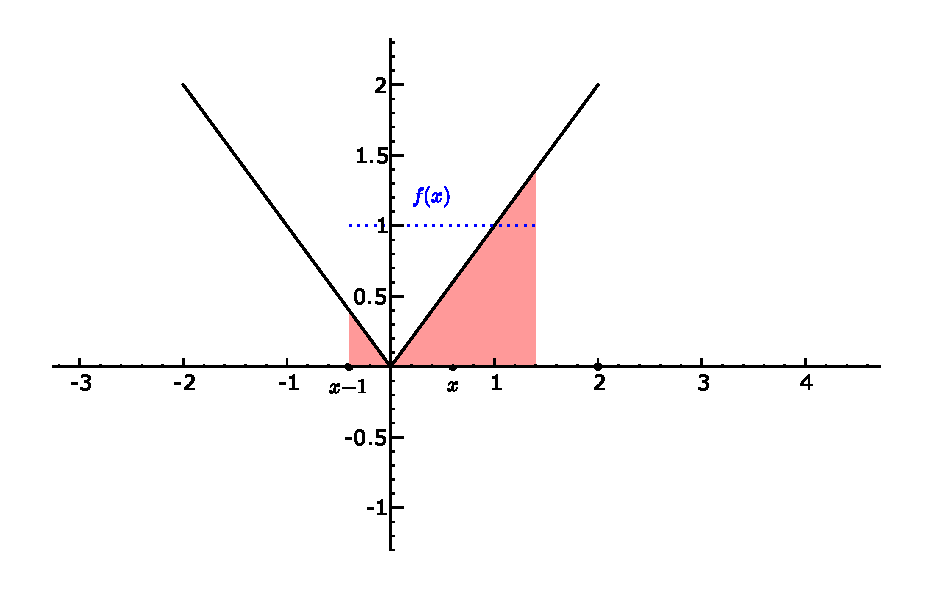
\includegraphics[width=\textwidth]{$HOME/book/fourier/img/19May2008img3.eps}
\caption{For $0\leq x\leq 1$}\label{img:19May2008:img3}
\end{figure}

We then find
\begin{equation}
(f*g)(x) = \begin{cases} x^2+1, &|x|\leq1\\
2 - \frac{1}{2}(|x|-1)^2, & 1\leq|x|\leq3\\
0 &\text{otherwise}.
\end{cases}
\end{equation}
The Fourier transform is then
\begin{equation}
\mathcal{F}[(f*g)] = \int^{1}_{-1}( x^2+1)e^{-i\xi x}dx + \int_{1\leq|x|\leq3}(2
- \frac{1}{2}(|x|-1)^2)e^{-i\xi x}dx
\end{equation}
This is a bit of a difficult thing to evaluate, so perhaps
we shouldn't even try.

On the other hand, we can find
\begin{equation}
\mathcal{F}[f] = \widehat{f}(\xi) = 2\frac{\sin(\xi)}{\xi}
\end{equation}
and similarly
\begin{subequations}
\begin{align}
\int^{A}_{0}xe^{-i\xi x}dx &= \frac{ix}{\xi}e^{-i\xi
  x}\Big|^{A}_{0} - \frac{i}{\xi}\int^{A}_{0}e^{-i\xi x}dx\\
&= \frac{iA}{\xi}e^{-iA\xi} - \frac{1}{\xi^2} + \frac{1}{\xi^2}e^{-iA\xi}\\
&= \left(\frac{1}{\xi^2} + \frac{iA}{\xi}\right)e^{-iA\xi} - \frac{1}{\xi^2}\\ 
\mathcal{F}[g] &= \int^{2}_{0}xe^{-i\xi x}dx -\int^{0}_{-2}xe^{-i \xi x}dx\\ 
&= \int^{2}_{0}xe^{-i\xi x}dx +\int^{-2}_{0}xe^{-i \xi x}dx\\ 
&= \left(\frac{1}{\xi^2}+\frac{i2}{\xi}\right)e^{-i2\xi} +
\left(\frac{1}{\xi^2} - \frac{i2}{\xi}\right)e^{i2\xi} -
\frac{2}{\xi^2}\\
&= \frac{2\cos(2\xi)}{\xi^2} + \frac{4\sin(2\xi)}{\xi} - \frac{2}{\xi^2}
\end{align}
\end{subequations}
Thus
\begin{equation}
\mathcal{F}[f*g] = \widehat{f}(\xi)\widehat{g}(\xi) =
  \left(2\frac{\sin(\xi)}{\xi}\right)\left[\frac{2\cos(2\xi)}{\xi^2} + \frac{4\sin(2\xi)}{\xi} - \frac{2}{\xi^2}\right]
\end{equation}
which would have been an impossible integral to perform if
we did it the direct, naive way.
\end{ex}
\subsection{Applications of the Fourier Transform}

\marginpar{Applications: Differential Equations}One of the most useful applications of the Fourier transform
is to solve differential equations. Usually, it is on
unbounded domains. What does this mean? Well, if the
function has boundaries of $(-\infty,\infty)$, or
$(-\infty,0)$, or $(0,\infty)$, then it's domain is
unbounded.\index{Fourier Transform!Solving Differential Equations}

\begin{ex}{(Heat Equation)}\index{Heat Equation!Solved Using Fourier Transform}
The heat equation is
\begin{equation}
\partial_{t}u(x,t) =
k\partial_{x}^{2}u(x,t),\quad-\infty\leq x\leq\infty.
\end{equation}
There is no boundary condition for $u$ but we have the
initial condition $u(x,0)=f(x)$. We can take the Fourier
transform in the $x$ variable to find
\begin{equation}
\partial_{t}\widehat{u}(\xi,t) = k(i\xi)^2\widehat{u}(\xi,t)
= -k\xi^{2}u(\xi,t)
\end{equation}
This is a first order differential equation in time, which
has the solution
\begin{equation}
\widehat{u}(\xi,t) = \widehat{f}(\xi)e^{-k\xi^2t}
\end{equation}
If we define
\begin{equation}
K_{t}(x) = \mathcal{F}^{-1}[e^{-k\xi^2t}] =
\frac{1}{\sqrt{4\pi kt}}e^{-x^2/(4kt)}
\end{equation}
(where we just used our relation of the Fourier transform of
the Gaussian to justify this), then
\begin{equation}
\widehat{u}(\xi,t) = \mathcal{F}[f*K_{t}]
\end{equation}
thus
\begin{equation}
u(x,t) = (f*K_{t})(x) = \frac{1}{\sqrt{4\pi kt}}\int f(y)e^{-(x-y)^{2}/4kt}dy.
\end{equation}
\end{ex}
\begin{ex}{(Wave Equation)}\index{Wave Equation!Solve With Fourier Transform}
The wave equation for an unbounded wave is
\begin{equation}
\partial_{x}^{2}u(x,y) + \partial_{y}^{2}u(x,y) = 0,\quad
-\infty<x<\infty,\quad y>0
\end{equation}
We would like to look for bounded solutions. So we take the
Fourier transform in $x$ and find
\begin{equation}
-\xi^2\widehat{u}+\partial_{y}^{2}\widehat{u} = 0
\end{equation}
The initial condition becomes
$\widehat{u}(\xi,0)=\widehat{f}(\xi)$. So we've changed the
wave equation into a second order ODE, the characteristic
equation is
\begin{equation}
-\xi^2 + r^2 = 0\Rightarrow r=\pm|\xi|.
\end{equation}
So, the general solution is
\begin{equation}
\widehat{u}(\xi,y) = c_{1}(\xi)e^{|\xi|y} + c_{2}(\xi)e^{-|\xi|y}
\end{equation}
Observe that as $\xi\to\pm\infty$, the first term goes to
infinity. So, due to our demand of making $u$ bounded, we
need to set $c_1=0$. Thus our solution becomes (by imposing
our initial condition)
\begin{subequations}
\begin{align}
\widehat{u}(\xi,y) &= c_{2}(\xi)e^{-|\xi|y}\\
&= \widehat{f}(\xi)e^{-|\xi|y}.
\end{align}
\end{subequations}
Once again, this is a Fourier transform of $f$ convoluted
with some function. We then write
\begin{equation}
\widehat{u}(\xi,y) = \widehat{f}(\xi)e^{-|\xi|y} = \mathcal{F}[f*P_y]
\end{equation}
so we define
\begin{equation}
P_{y}(x) = \mathcal{F}^{-1}[e^{-|\xi|y}]
\end{equation}
which is a special function. We call it the \textbf{Poisson Kernel}\index{Poisson Kernel}
and we can write it out explicitly as
\begin{equation}
  \addtolength{\fboxsep}{5pt}
   \boxed{
   \begin{gathered}
     P_{y}(x) = \frac{y}{\pi(x^2+y^2)}.
   \end{gathered}
   }
\end{equation}
We can now write the general solution of the wave equation
as
\begin{equation}
u(x,y) = (f*P_y)(x) = \int\frac{yf(x-y)}{\pi(x^2+y^2)}dy.
\end{equation}
This concludes our example.
\end{ex}

\marginpar{Applications: Signal Analysis}The other application is signal analysis. We represent a
signal as a function of time, $f(t)$, representing the
amplitude of a signal at time $t$ (e.g. a sound signal,
$f(t)$ would be the volume of the sound, etc.).

By the Fourier inversion formula
\begin{equation}
f(t) = \frac{1}{2\pi}\int e^{i\omega
  t}\widehat{f}(\omega)d\omega
\end{equation}
where $\widehat{f}(\omega)$ is the Fourier transform
\begin{equation}
\widehat{f}(\omega) = \int f(t)e^{-i\omega t}dt
\end{equation}
where $t$ is time, and $\omega$ is frequency; we have $t$ in
units of (e.g) seconds, and $\omega$ in units of Herz
(``cycles per second'').

The Fourier inversion represents $f(t)$ as a (continuous) superposition
of periodic and simple waves. That is
\begin{equation}
e^{i\omega t} = \text{ periodic simple waves}
\end{equation}
and
\begin{equation}
\mathcal{F}^{-1}[\widehat{f}(\omega)] = \begin{pmatrix}
$representation$\ $of$\ f(t)\ $as$\\
$continuous$\ $superposition$\ $of$\\
$simple$\ $periodic$\ $waves$.
\end{pmatrix}.
\end{equation}

We also model systems (e.g. an electrical system, or a
telephone system) with an operator $L$
\begin{align*}
L:&f\to L[f]\\
&\text{input}\to\text{output}
\end{align*}
When $L$ is linear, we have a linear system. If $L$ is
shift-invariant, then $L$ commutes with translations. What
do we mean by this? Well, if
\begin{equation}
L[f(x)]=g(x)\Rightarrow L[f(x+k)] = g(x+k)
\end{equation}
for some arbitrary constant $k$, then an operator that
shifts $f$ by 1
\begin{equation}
E[f(x)] = f(x+1)
\end{equation}
can be interchanged with $L$:
\begin{equation}
L[E[f(x)]]=E[L[f(x)]].
\end{equation}
For instance, the AM radio operator is a linear, shift
invariant system. 

\part{Discrete Fourier Transforms}
\section{Sampling Theorem}
%%
%% 21May2008.tex
%% 
%% Made by Alex Nelson
%% Login   <alex@tomato>
%% 
%% Started on  Sat Dec 27 17:17:37 2008 Alex Nelson
%% Last update Sat Dec 27 17:17:37 2008 Alex Nelson
%%

Oftentimes in signal processing, we have to work with
discrete packets instead of continuous signals. Because of
this, we often use a discretized Fourier transform. We will
introduce a few notions first before getting to the Discrete
Fourier transform.

\begin{defn}\index{Signal!Bandlimited}
A signal $f(t)$ is \textbf{bandlimited} if
$\widehat{f}(\omega)$ vanishes for all $|\omega|>\Omega$
where $\Omega$ is a constant called the \textbf{bandwidth}.
\end{defn}

\begin{samplingthm}\index{Sampling Theorem}
Suppose $f\in L^2$ and $\widehat{f}(\omega)=0$ for
$|\omega|>\Omega$.\marginpar{So we can have a function defined on
  the real line, and can be reconstructed from countably many
  values we know about it, \emph{despite} it having uncountably
  many values.} Then
\begin{equation}
f(t) =
\sum^{\infty}_{n=-\infty}f\left(\frac{n\pi}{\Omega}\right)\frac{\sin(\Omega t - n\pi)}{\Omega t - n\pi}.
\end{equation}
We may interpret the sine function as the orthogonal basis in
$L^2$ where $\{\widehat{f}(\omega)=0$ for $|\omega|>\Omega\}$ is
a subspace of $L^{2}$ (i.e. it is closed under function addition
and scalar multiplication).
\end{samplingthm}
\begin{proof}
Since $f\in L^2$, $\widehat{f}\in L^2(-\Omega,\Omega)$ so we
may expand $\widehat{f}$ in a Fourier series! We have to
extend $\widehat{f}$ to be periodic, and then look at the
particular interval of interest $(-\Omega,\Omega)$. Now the
Fourier series of the function is
\begin{equation}
\widehat{f}(\omega) = \sum^{\infty}_{n=-\infty}c_{-n}e^{-in\omega\pi/\Omega}
\end{equation}
and further
\begin{subequations}
\begin{align}
c_{-n} &= \frac{1}{2\Omega}\int^{\Omega}_{-\Omega}\widehat{f}(\omega)e^{in\omega\pi/\Omega}d\omega\\
&=
\frac{1}{2\Omega}\int^{\infty}_{-\infty}\widehat{f}(\omega)e^{in\omega\pi/\Omega}d\omega\text{  (extending from $[-\Omega,\Omega]$ to $\mathbb{R}$)}\\
&= \frac{\pi}{\Omega}\left(\frac{1}{2\pi}\int^{\infty}_{-\infty}\widehat{f}(\omega)e^{in\omega\pi/\Omega}d\omega\right)\\
&=\frac{\pi}{\Omega}\left[f\left(\frac{n\pi}{\Omega}\right)\right]
= \frac{\pi}{\Omega}f\left(\frac{n\pi}{\Omega}\right)
\end{align}
\end{subequations}
which is really just the inverse Fourier Transform. Thus we have
\begin{equation}
\widehat{f}(\omega) = \sum^{\infty}_{n=-\infty}\frac{\pi}{\Omega}f\left(\frac{n\pi}{\Omega}\right)e^{-in\omega\pi/\Omega}
\end{equation}
We then perform the inverse Fourier transform to get
\begin{subequations}
\begin{align}
f(t) &=
\frac{1}{2\pi}\int^{\Omega}_{-\Omega}\widehat{f}(\omega)e^{i\omega t}d\omega\\
&=\frac{1}{2\Omega}\int^{\Omega}_{-\Omega}\left(\sum^{\infty}_{n=-\infty}f\left(\frac{n\pi}{\Omega}\right)e^{-in\omega\pi/\Omega}\right)e^{i\omega t}d\omega\\
&=\frac{1}{2\Omega}\sum f\left(\frac{n\pi}{\Omega}\right)\int^{\Omega}_{-\Omega}e^{i\omega(t-n\pi/\Omega)}d\omega\\
&=\frac{1}{2\Omega}\sum f\left(\frac{n\pi}{\Omega}\right)
\Omega\left[
\frac{e^{i(\Omega t-n\pi)}-e^{-i(\Omega t-n\pi)}}{i(\Omega t-n\pi)}
\right]\\
&=\sum f\left(\frac{n\pi}{\Omega}\right)\frac{\sin(\Omega t-n\pi)}{(\Omega t-n\pi)}
\end{align}
\end{subequations}
This concludes our proof.
\end{proof}
Here we must emphasize\marginpar{\Huge{NOTE!\\$\star\star\star\star\star$}}
\begin{equation}
  \addtolength{\fboxsep}{5pt}
   \boxed{
   \begin{gathered}
     \widehat{f}(\omega) = \sum\frac{\pi}{\Omega}f\left(\frac{n\pi}{\Omega}\right)e^{-in\omega\pi/\Omega}
   \end{gathered}
   }
\end{equation}
If we sample at $N$ points equally distanced from each
other, letting $t_n = n(\pi/\Omega)$, we have
\begin{equation}
\widehat{f}(\omega) = \frac{\pi}{\Omega}\sum f(t_n)e^{-it_n\omega}
\end{equation}
We assume the sample points are periodic.

\subsection*{Dual Formulation For Sampling Frequency}

Suppose we have a signal $f\in L^2$ such that $f(t)=0$ for
$|t|>L>0$. Then we say the signal is \textbf{time
  limited}\index{Time Limited}\index{Signal!Time Limited}. Then
\begin{equation}
\widehat{f}(\omega) = \sum^{\infty}_{-\infty}\widehat{f}\left(\frac{n\pi}{L}\right)\frac{\sin(L\omega-n\pi)}{(L\omega-n\pi)}.
\end{equation}
We then have a small modification to the Sampling Theorem.

\begin{thm}{\textbf{(Modified Sampling Theorem)}}
Suppose we have $f\in L^2$ and $\widehat{f}(\omega)=0$ for
$\omega$ outside of $[a,b]$. Then
\begin{equation}
f(t) = \sum f\left(\frac{2\pi n}{b-a}\right)e^{-i\left(\frac{a+b}{b-a}\right)n\pi t}
\left[\frac{\sin\left(\left(\frac{b-a}{2}\right)t-n\pi\right)}{\left(\frac{b-a}{2}\right)t-n\pi}\right]
\end{equation}
\end{thm}


\section{Uncertainty Principle}
%%
%% 23May2008.tex
%% 
%% Made by Alex Nelson
%% Login   <alex@tomato>
%% 
%% Started on  Sat Mar 28 16:11:02 2009 Alex Nelson
%% Last update Sat Mar 28 16:11:02 2009 Alex Nelson
%%
There is one last significant principle that we will cover in
signal processing -- Heisenberg's famous uncertainty principle.

\begin{defn}\index{Dispersion}
For $f\in L^2$, the \textbf{dispersion of $f$ about a point $a$}
is defined as
\begin{equation}
\Delta_{a}f = \frac{\int(x-a)^2|f(x)|^2dx}{\int|f(x)|^2dx}.
\end{equation}
\end{defn}
This tells us how concentrated the function $f$ is near the point
$a$. The smaller it is, the more concentrated $f$ is; the larger
it is, the less concentrated $f$ is.

\begin{ex}
Consider the rectangle function $\chi_{1/2}(t)$ which is 1 if
$t\in[-1/2,1/2]$ and 0 otherwise. We can explicitly compute
\begin{subequations}
\begin{align}
\Delta_{a}\chi_{1/2} &=
\frac{\int^{1/2}_{-1/2}(x-a)^2|\chi_{1/2}(x)|^2dx}{\int^{1/2}_{-1/2}|\chi_{1/2}(x)|^2dx}\\
&= \int^{1/2}_{-1/2}(x-a)^2dx\\
&= \frac{1}{3}(x-a)^{3}|^{x=1/2}_{x=-1/2}\\
&= a^{2}+\frac{1}{12}.
\end{align}
\end{subequations}
Note its smallest at $a=0$ and it increases as $|a|\to\infty$. 
\end{ex}

\begin{thm}{(Heisenberg's Uncertainty Principle)}\index{Uncertainty!Heisenberg}\index{Heisenberg!Uncertainty}
Given some $f\in L^2$, then
\begin{equation}
\left(\Delta_{a}f\right)\left(\Delta_{\alpha}\widehat{f}\right)\geq\frac{1}{4}
\end{equation}
for any $a,\alpha\in\mathbb{R}$.
\end{thm}
This amounts to nothing more than saying ``For any signal $f\in
L^2$, $f$ \emph{cannot} be \emph{both} time limited and band limited.''

%\input{tex/28May2008}
%\input{tex/30May2008}
%\input{tex/2June2008}
%\input{tex/6June2008}
\nocite{morseVolOne}
\nocite{textbook}

\addcontentsline{toc}{section}{References} 
\bibliographystyle{utphys}
\bibliography{foo}
\printindex
\end{document}
